\chapter{Numerical Results and Discussion} \label{chap:results}
We present numerical results based in the implementation suggested in \chapref{chap:implementation} for the models derived in \chapref{chap:modeling}. It is constructed four sets of test problems with the goal of demonstrating different strengths and weaknesses of the purposed models. All three models will be tested on all test cases and we present the resulting stationary curve in addition to information about the transitional movement from initial to stationary curve.

As the objective of this thesis is mostly to investigate level set methods, we have no real world data, and no objective quality measures for our solution. Thus, the parameters used in the following results are not selected to produce an optimal curve by any measures, and some parameter choices are even included to show what can go wrong.

\section{Test Cases}
The intentions of the test cases is to demonstrate the performance of the models when the set of points are irregular or noisy as is the goal of the thesis. In addition we want to test the numerical results compared to the analytical circular analysis and we want to observe how the different parameters influences the solutions.

The four sets of sample points are displayed in \figref{fig:test-cases}. The test case in \figref{fig:test-case-circle} is a point set consisting of $200$ points distributed in a circle with radius $0.5$. This is the same radius as the point set in the analysis of the radially symmetric example. This test case will show how well the implementation corresponds to the presented theory.

\begin{figure}
  \begin{subfigure}[h]{0.25\linewidth}
    \centering
    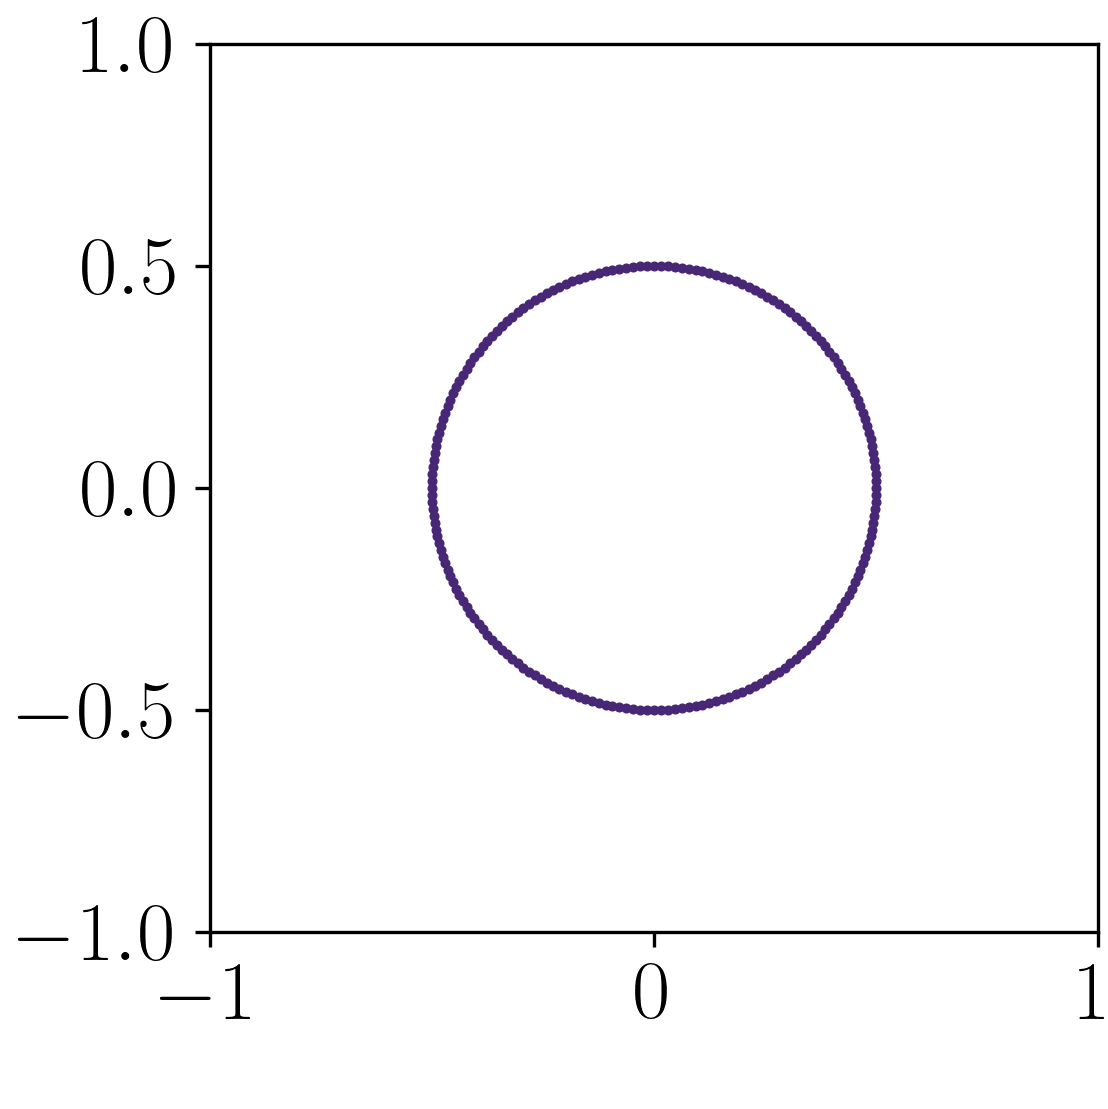
\includegraphics[width=0.9\linewidth]{figures/TestCases/Circlepoints.png}
    \caption{Circle}
    \label{fig:test-case-circle} 
    \vspace{1em}
  \end{subfigure}%% 
  \begin{subfigure}[h]{0.25\linewidth}
    \centering
    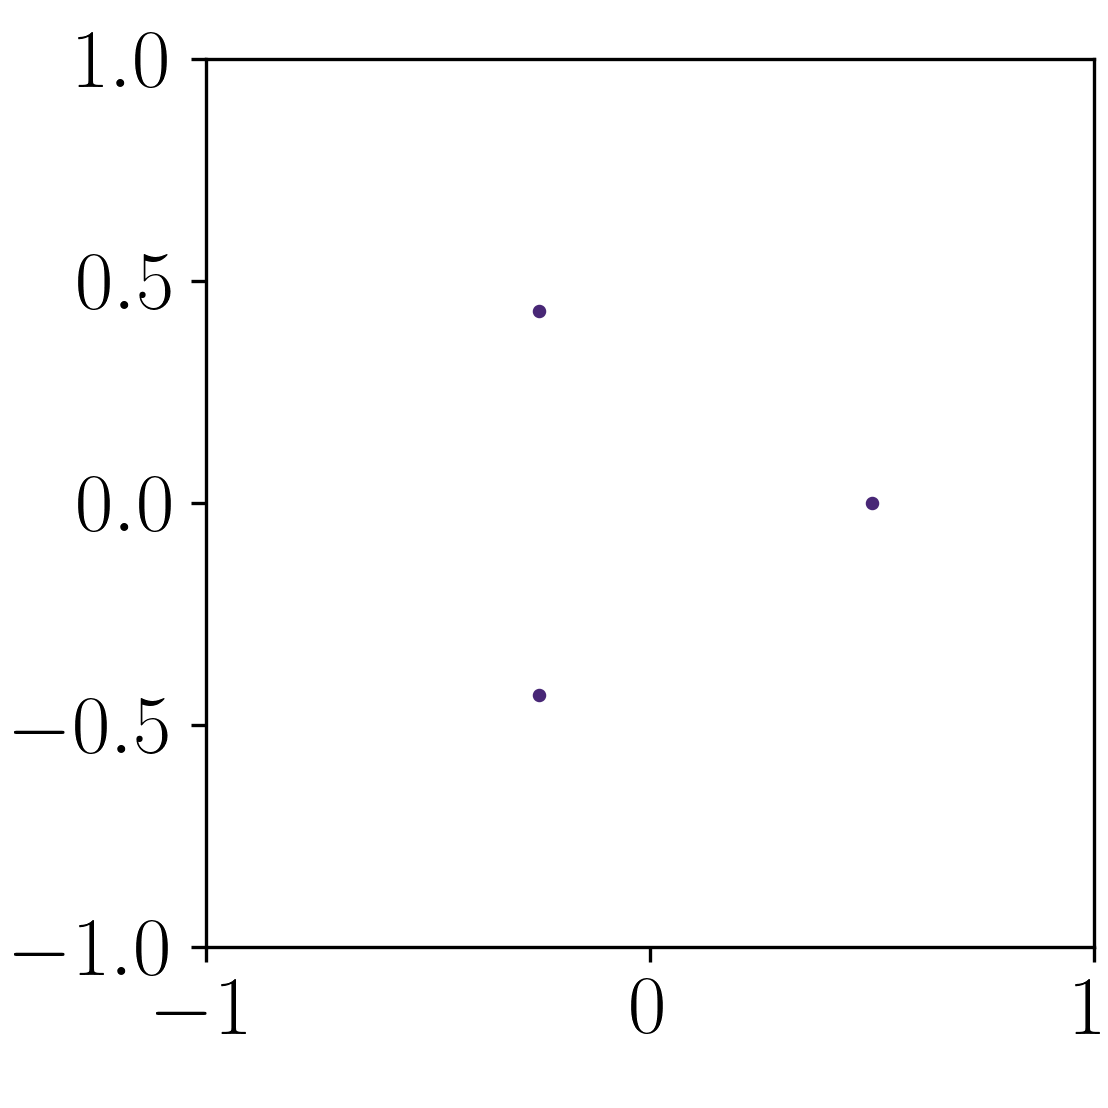
\includegraphics[width=0.9\linewidth]{figures/TestCases/Fewpoints.png} 
    \caption{Three points}
    \label{fig:test-case-few} 
    \vspace{1em}
  \end{subfigure} 
  \begin{subfigure}[h]{0.25\linewidth}
    \centering
    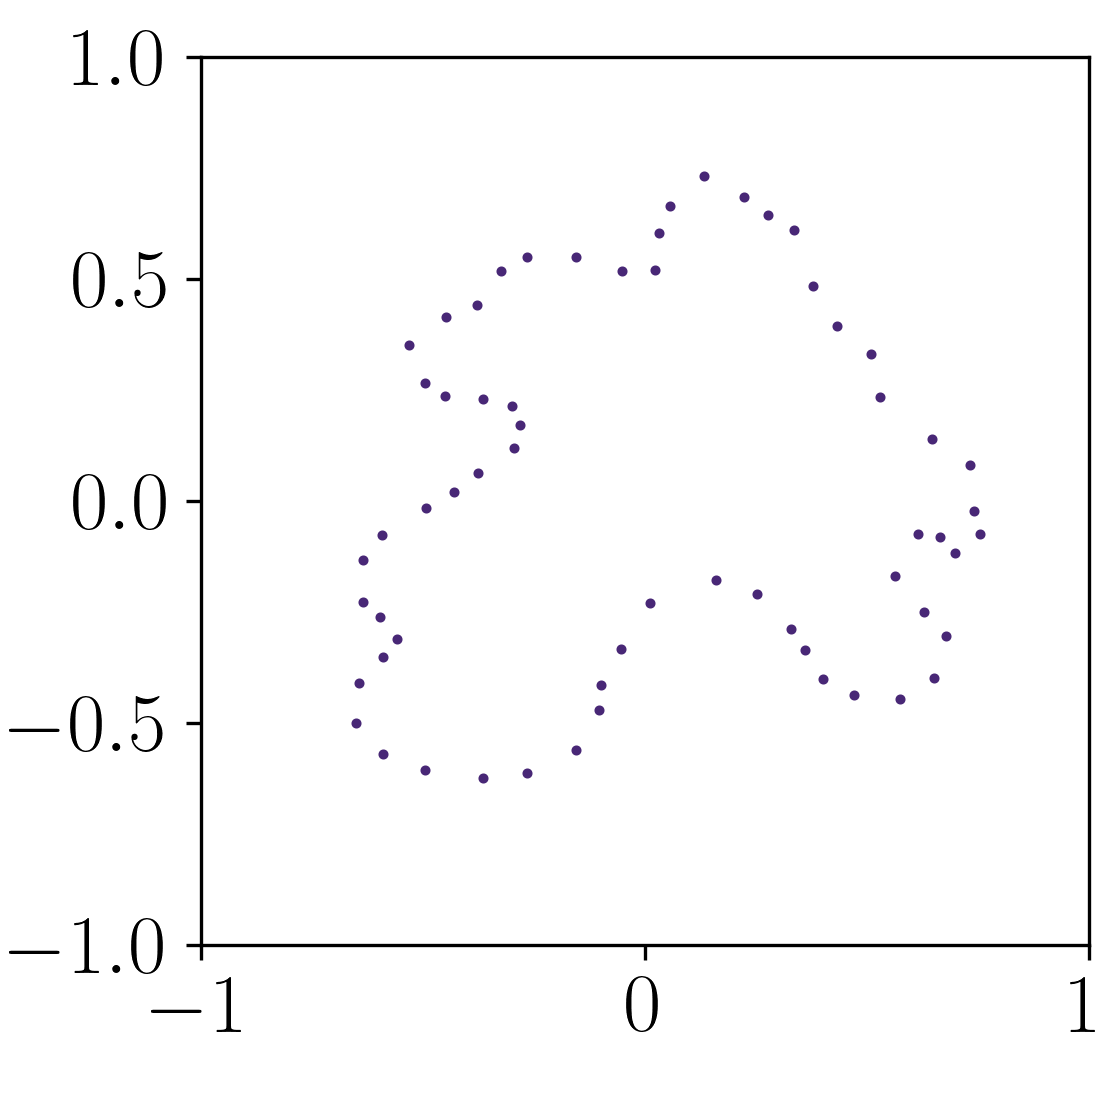
\includegraphics[width=0.9\linewidth]{figures/TestCases/Manypoints.png} 
    \caption{Manufactured shape}
    \label{fig:test-case-many} 
  \end{subfigure}%%
  \begin{subfigure}[h]{0.25\linewidth}
    \centering
    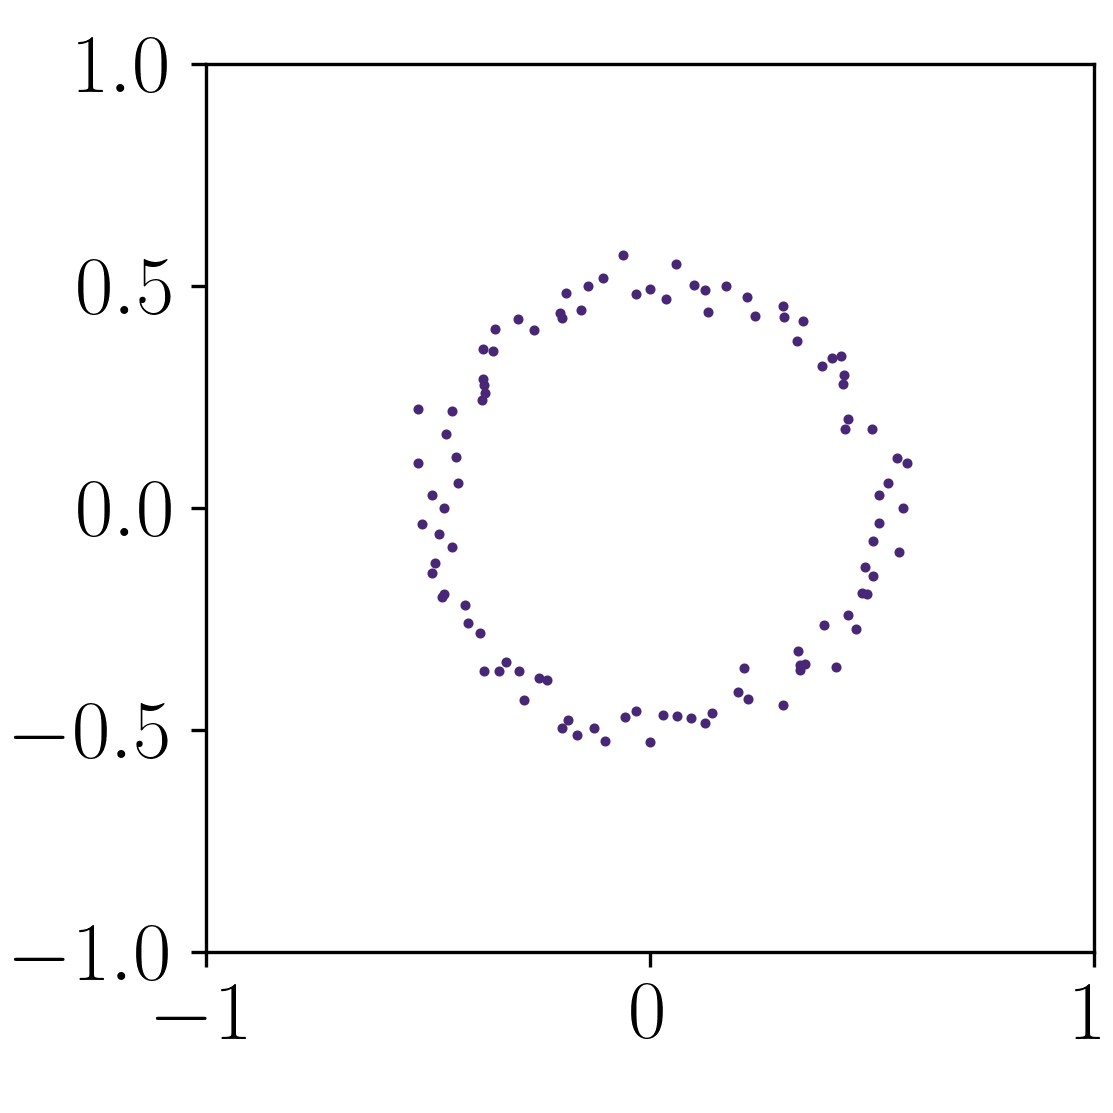
\includegraphics[width=0.9\linewidth]{figures/TestCases/Noisypoints.png}
    \caption{Noisy circle}
    \label{fig:test-case-noisy} 
    \vspace{1em}
  \end{subfigure} 
  \caption[All Test Cases]{The four sets of sample points used to produce the results presented in this chapter.}
  \label{fig:test-cases} 
\end{figure}

The point set displayed in \figref{fig:test-case-few} consists only of three points with equal spacing. The purpose of this example is to show how the curvature and distance is related for the three models when the distance can not be small at all points on the curve. 

In \figref{fig:test-case-many} the points are distributed dense enough such that the underlying shape is imaginable such that we can to some degree envision what an optimal solution should look like. At the same time, the shape includes concave and convex regions of different curvatures\todo{Kan jeg si kurvatur om et punktsett?} which is interesting to see how the models manages.

The last test case is constructed to demonstrate how the models handles noisy and irregular data. The radius is $0.5$ identical to the first test case, but noise is added by sampling a normal distribution with standard deviation of $SD=0.08$.

\section{Test Case 1: Circle of Dense Points}
We begin presentation of the result with model 1, stated in \eqref{eq:model1-pde}. In order to compare the theoretical behavior with the numerical result, we choose $\alpha=0.96$ compatible with the analytical streamlines from \figref{fig:total-streamline-picture}. Before we begin the discussion of our results, we explain the plots that will be used throughout this chapter.

In \figref{fig:model1-sigma-dist-full}, shows the evolution of the zero level curve over time. To the left, we can see a plot of zero level curves at different times where the opacity of the curve line increases with time. The curves are sampled uniformly in time and hence the spacing of the curves will provide an impression of the velocity at different times. The convention will be to plot such a contour plot together with a plot like the one to the right showing the change since last re-initialization. This will be denoted as the residual plot.

\begin{figure}
\begin{center}
\resizebox{.99\textwidth}{!}{%
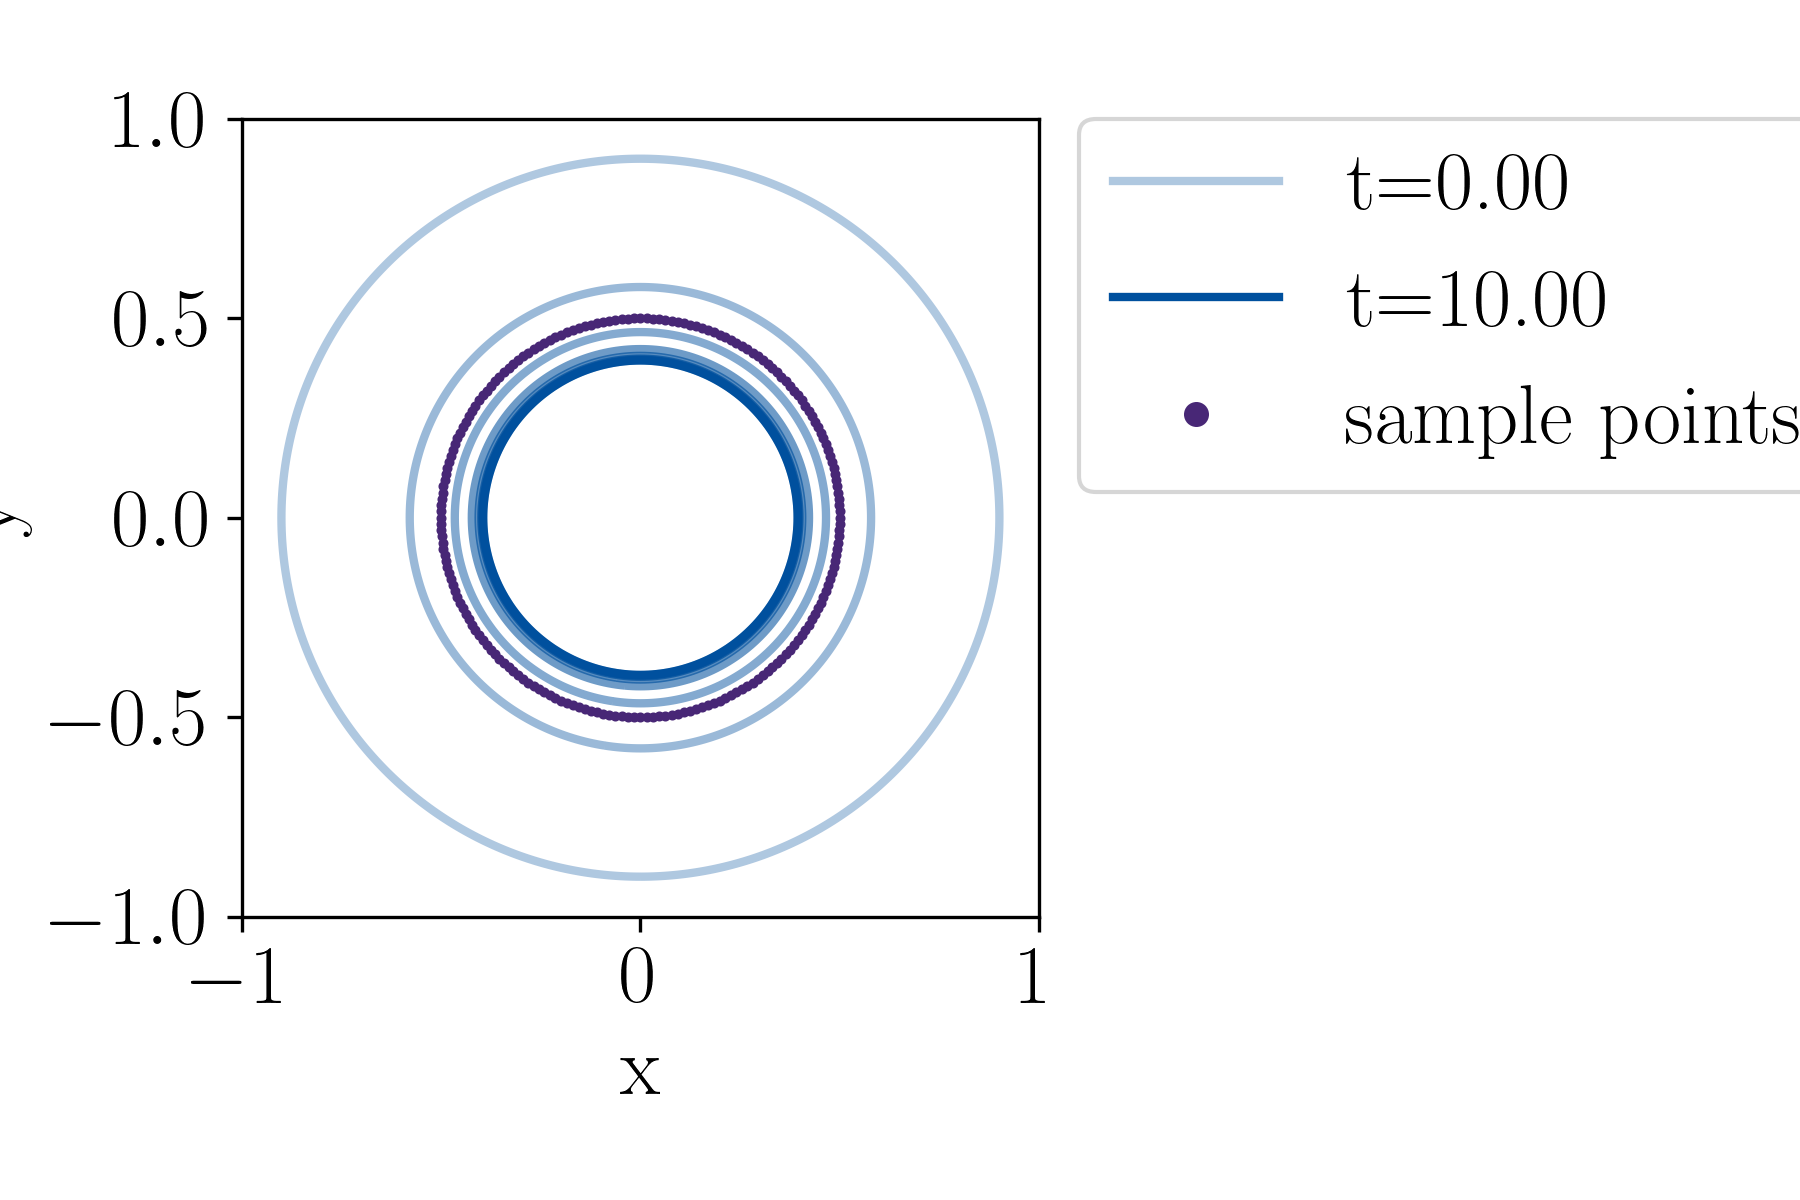
\includegraphics[height=3.5cm]{figures/Results/Circle/model1/circlepoints-a96.png}%
\,
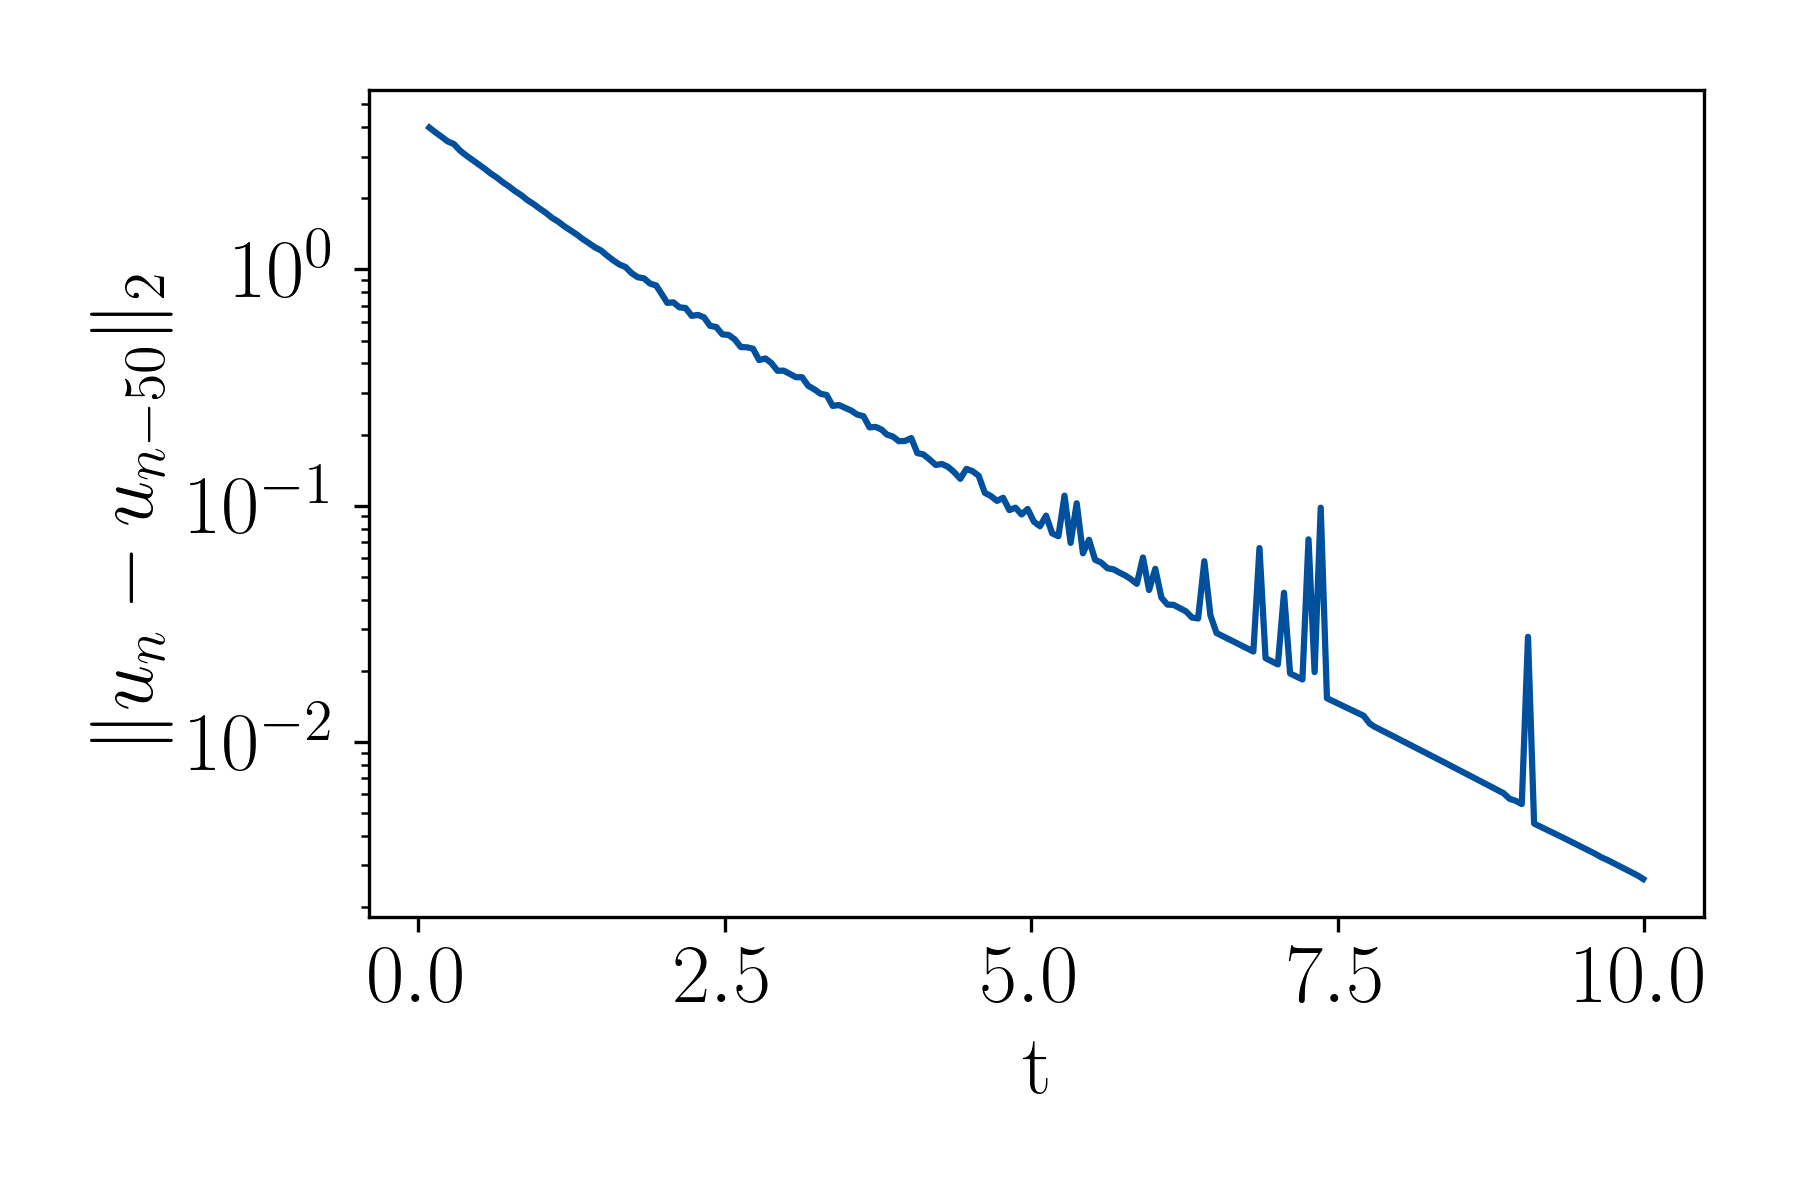
\includegraphics[height=3.5cm]{figures/Results/Circle/model1/circle-a096-logy.png}%
}
\end{center}
\vspace{-2.5em}
\caption[Model 1 - Circular example $\alpha=0.96$]{Model 1: $h=0.01$, $10$ level curves, $\alpha=0.96$, $dt=1/10h$, $r_0=0.9$, $200$ points. Sigma!! Reinitialized every $50$ iteration}
\label{fig:model1-sigma-dist-full}
\end{figure}

Now, on to the results. First of all, we note from \figref{fig:m1-circle-radius-numanal} that the evolution of the numerical solution, fits the evolution of the analytical solution perfectly. The end radius is not visible at the plot, but from calculating the radius from the last zero level curve, we get that $r(10)=0.3941$ which is not far from $r_f=0.39433$ calculated using \eqref{eq:stationary-radius} with $\alpha=0.96$. We see that we have an error in the $4$th decimal place, but this is not discouraging as the discretizations of the differential operators are only second order.

Moreover, we see from the residual plot in \figref{fig:model1-sigma-dist-full} that the curve do not stop moving entirely during the execution time, but the speed slows down as the radius approaches the analytical stationary radius. Furthermore, we see from the contour plot, that it only takes about $4$ level curves, which corresponds to $t\sim 4$ until the curve reaches a state where we can no longer see the difference. 


\begin{figure}
    \centering
    \begin{subfigure}[h]{0.49\textwidth}
        \centering
        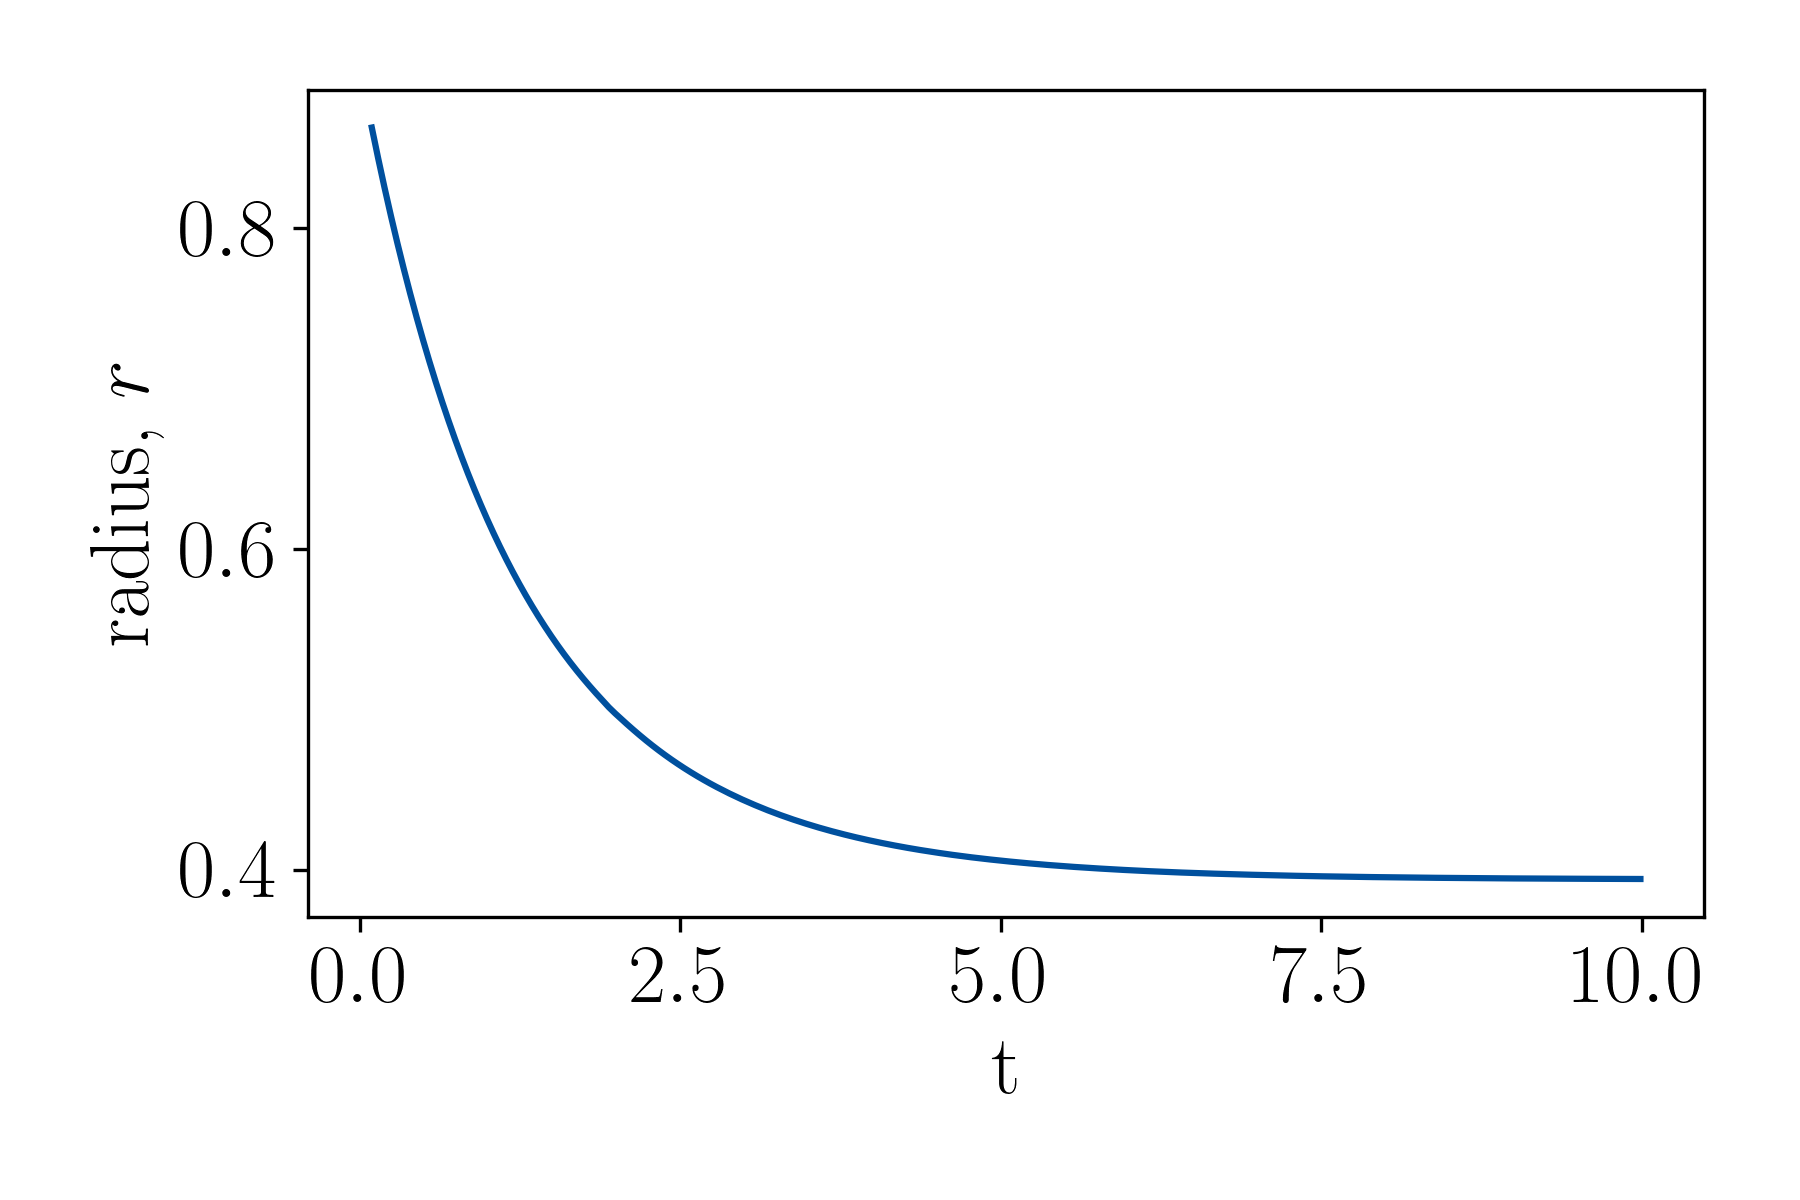
\includegraphics[width=\linewidth]{figures/Results/Circle/model1/circlepoints-a96-rad.png}
        \caption{Numerical solution}
        \label{fig:m1-circle-numerical-radius}
    \end{subfigure}%
    \begin{subfigure}[h]{0.49\textwidth}
        \centering
        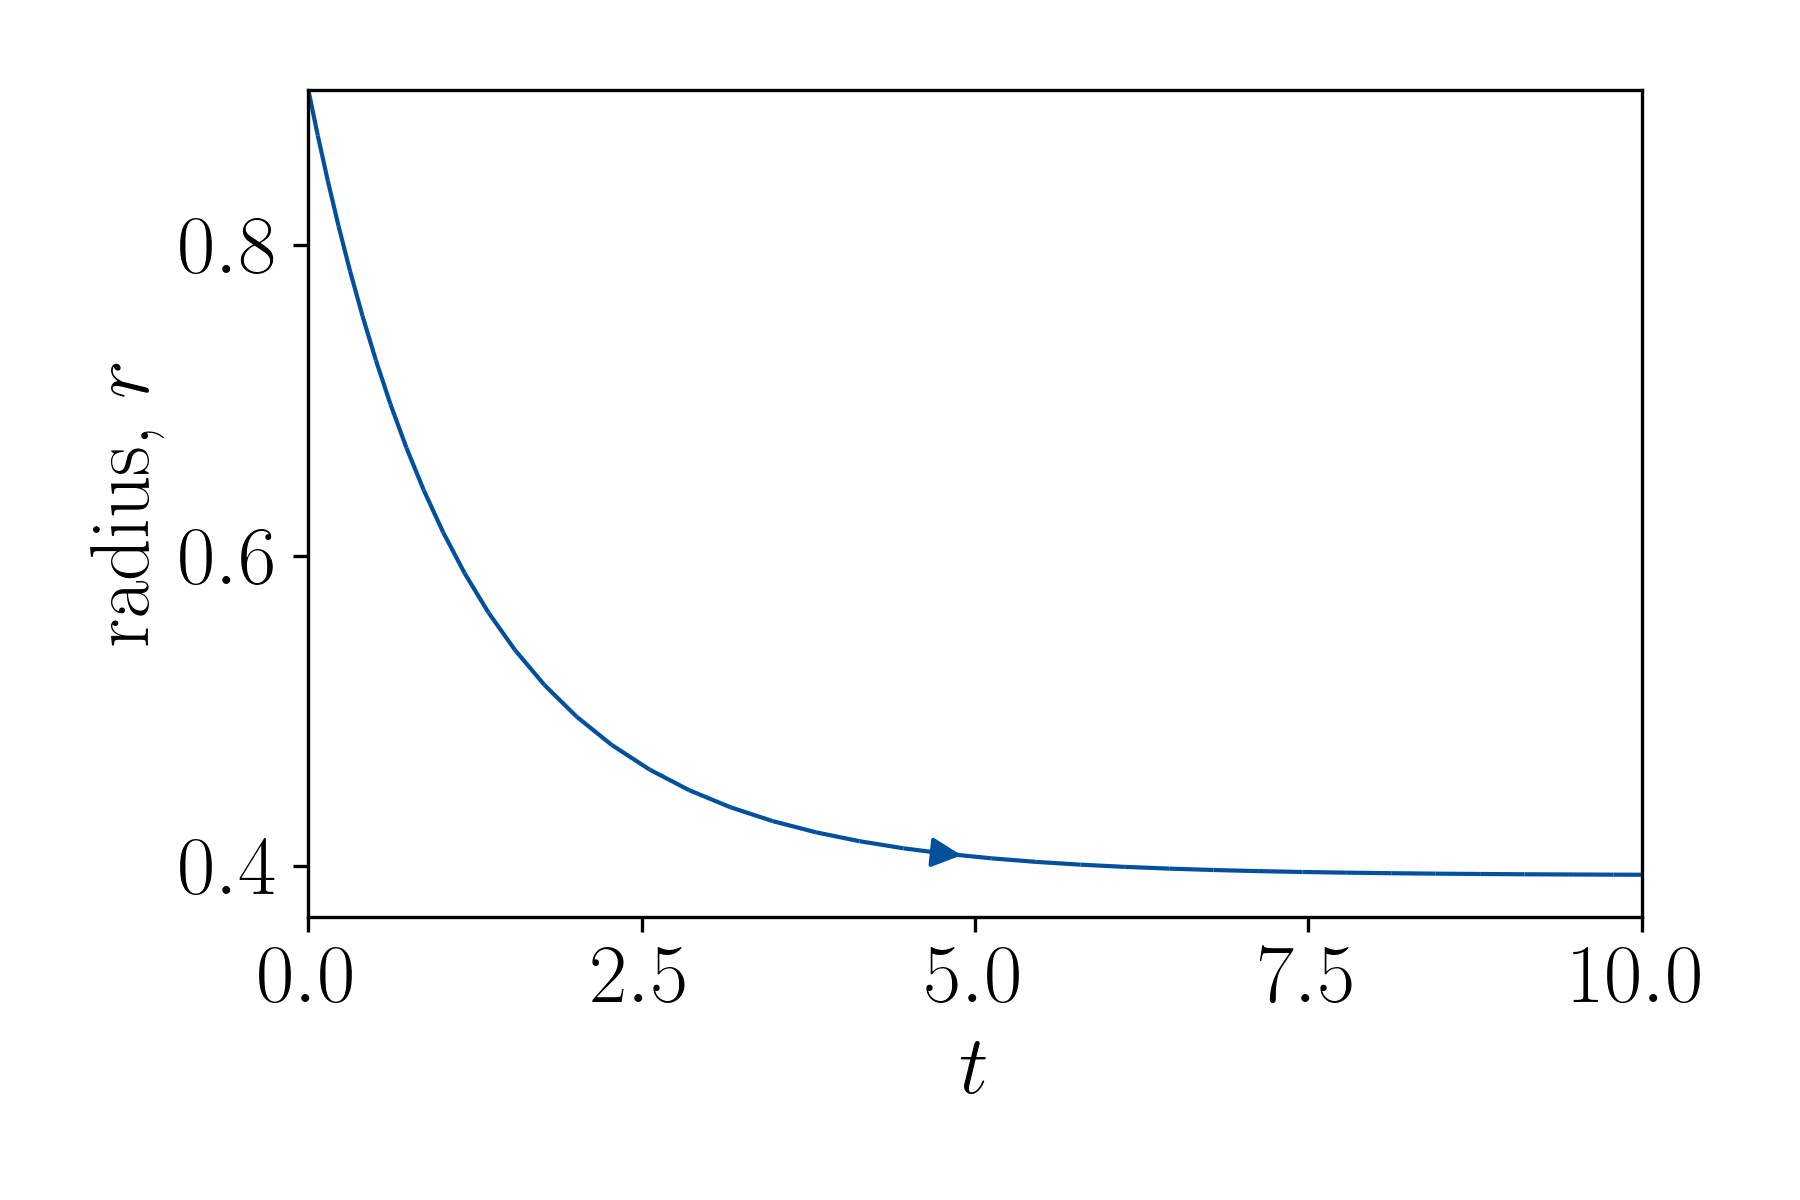
\includegraphics[width=\linewidth]{figures/Circle-radii/mod1-r09.png}
        \caption{Analytical streamline}
        \label{fig:m1-circle-analytical-radius}
    \end{subfigure}
    \caption[Model 1 - Circle, Radius]{The radius over time for respectively the numerical implementation of model 1 for a circle with $200$ points and the analytical movement following \eqref{eq:pde-streamline}. Both the analytical streamline and the numerical solution starts with an initial curve in $r_0=0.9$.}
    \label{fig:m1-circle-radius-numanal}
\end{figure}

Furthermore, to confirm the significance of the parameter $\alpha$. We run another simulation, increasing the parameter to $\alpha=0.99$. We see in \figref{fig:model1-a99} to the left that the radius is much more close to $r_v=0.5$. It is hard to see accurately what the radius is at $t=10$, but when calculating from the last zero iso-curve, yields $r(10)=0.4788$. When inserting all information into \eqref{eq:stationary-radius}, we obtain the theoretical stationary solution, $r_f=0.4789$. From the residual plot to the right in \figref{fig:model1-a99} we see that the curve moves slower for $\alpha=0.99$. This makes sense as it is the curvature that is the main drive close to the point set.

\begin{figure}
\begin{center}
\resizebox{.99\textwidth}{!}{%
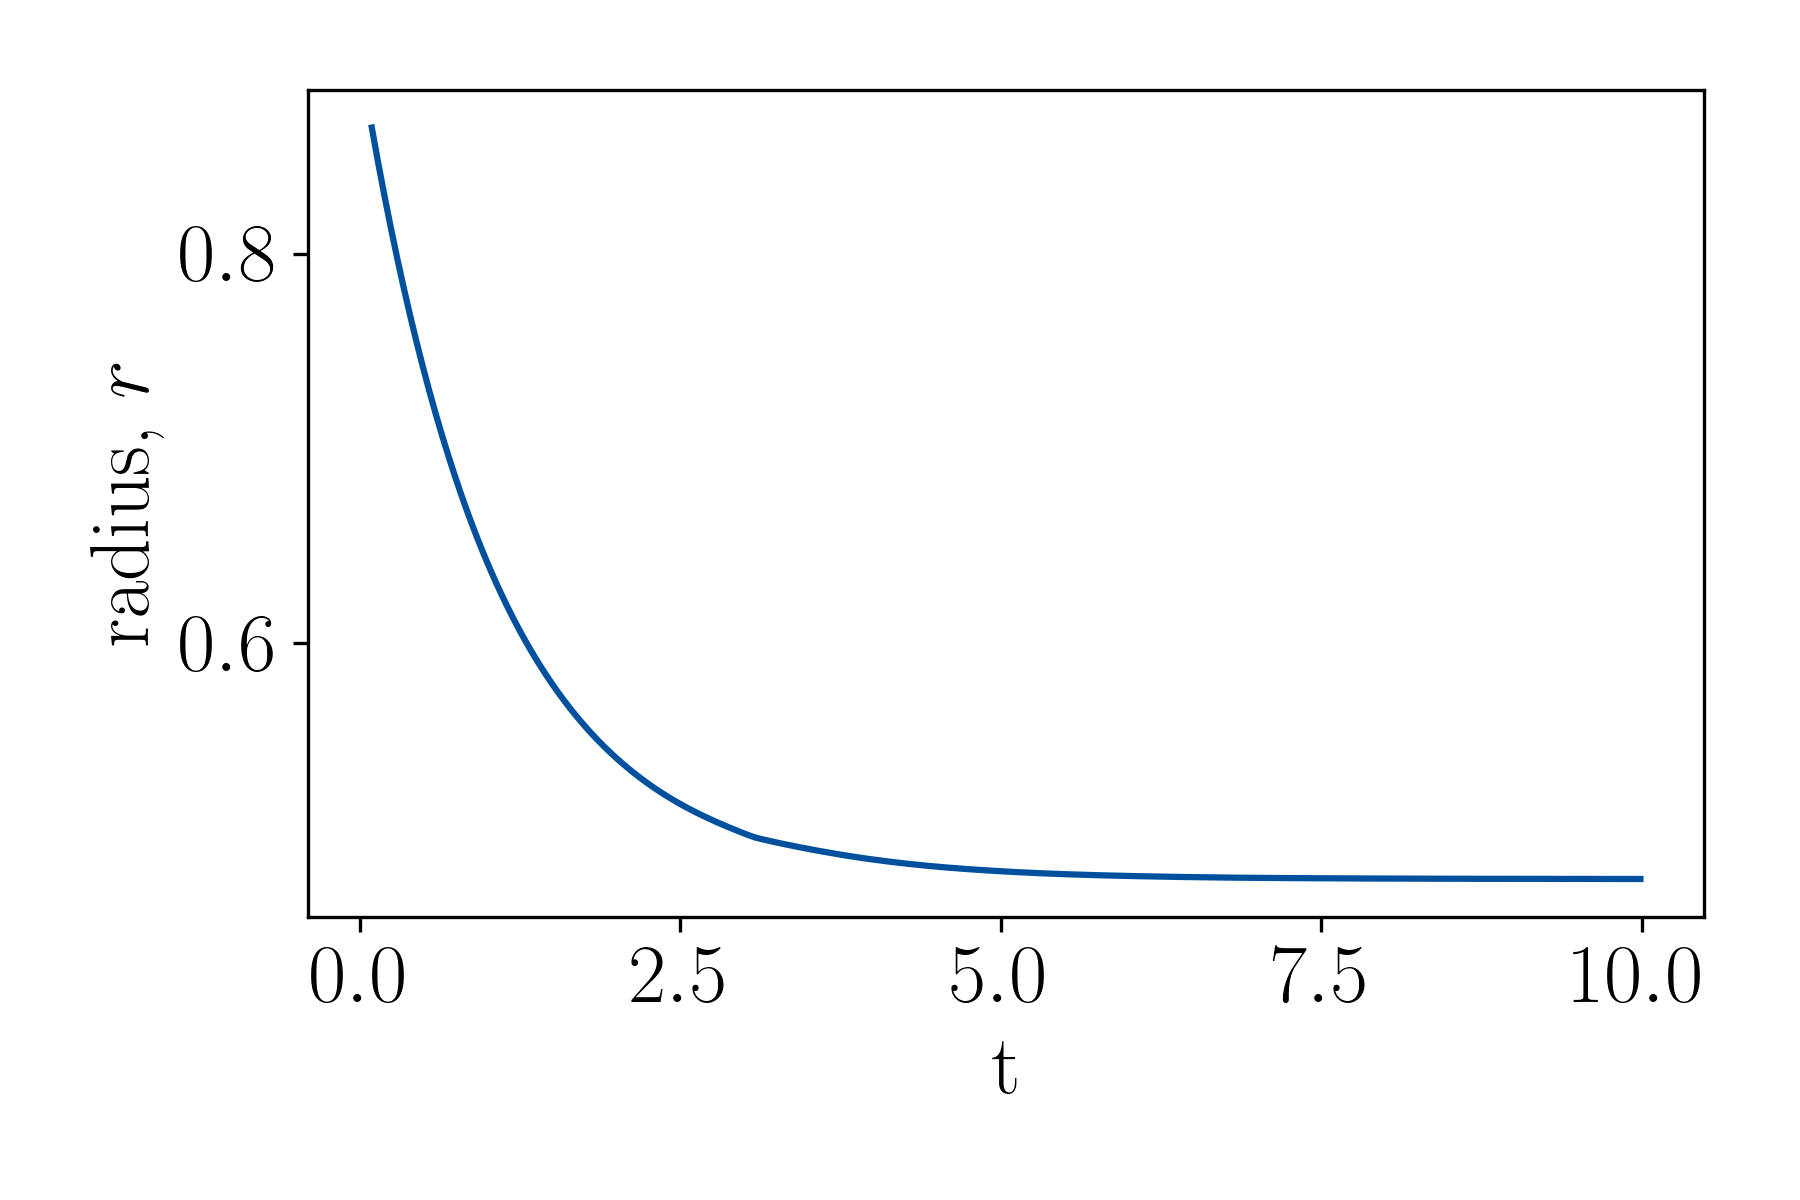
\includegraphics[height=3.5cm]{figures/Results/Circle/model1/circle-rad-099.png}%
\,
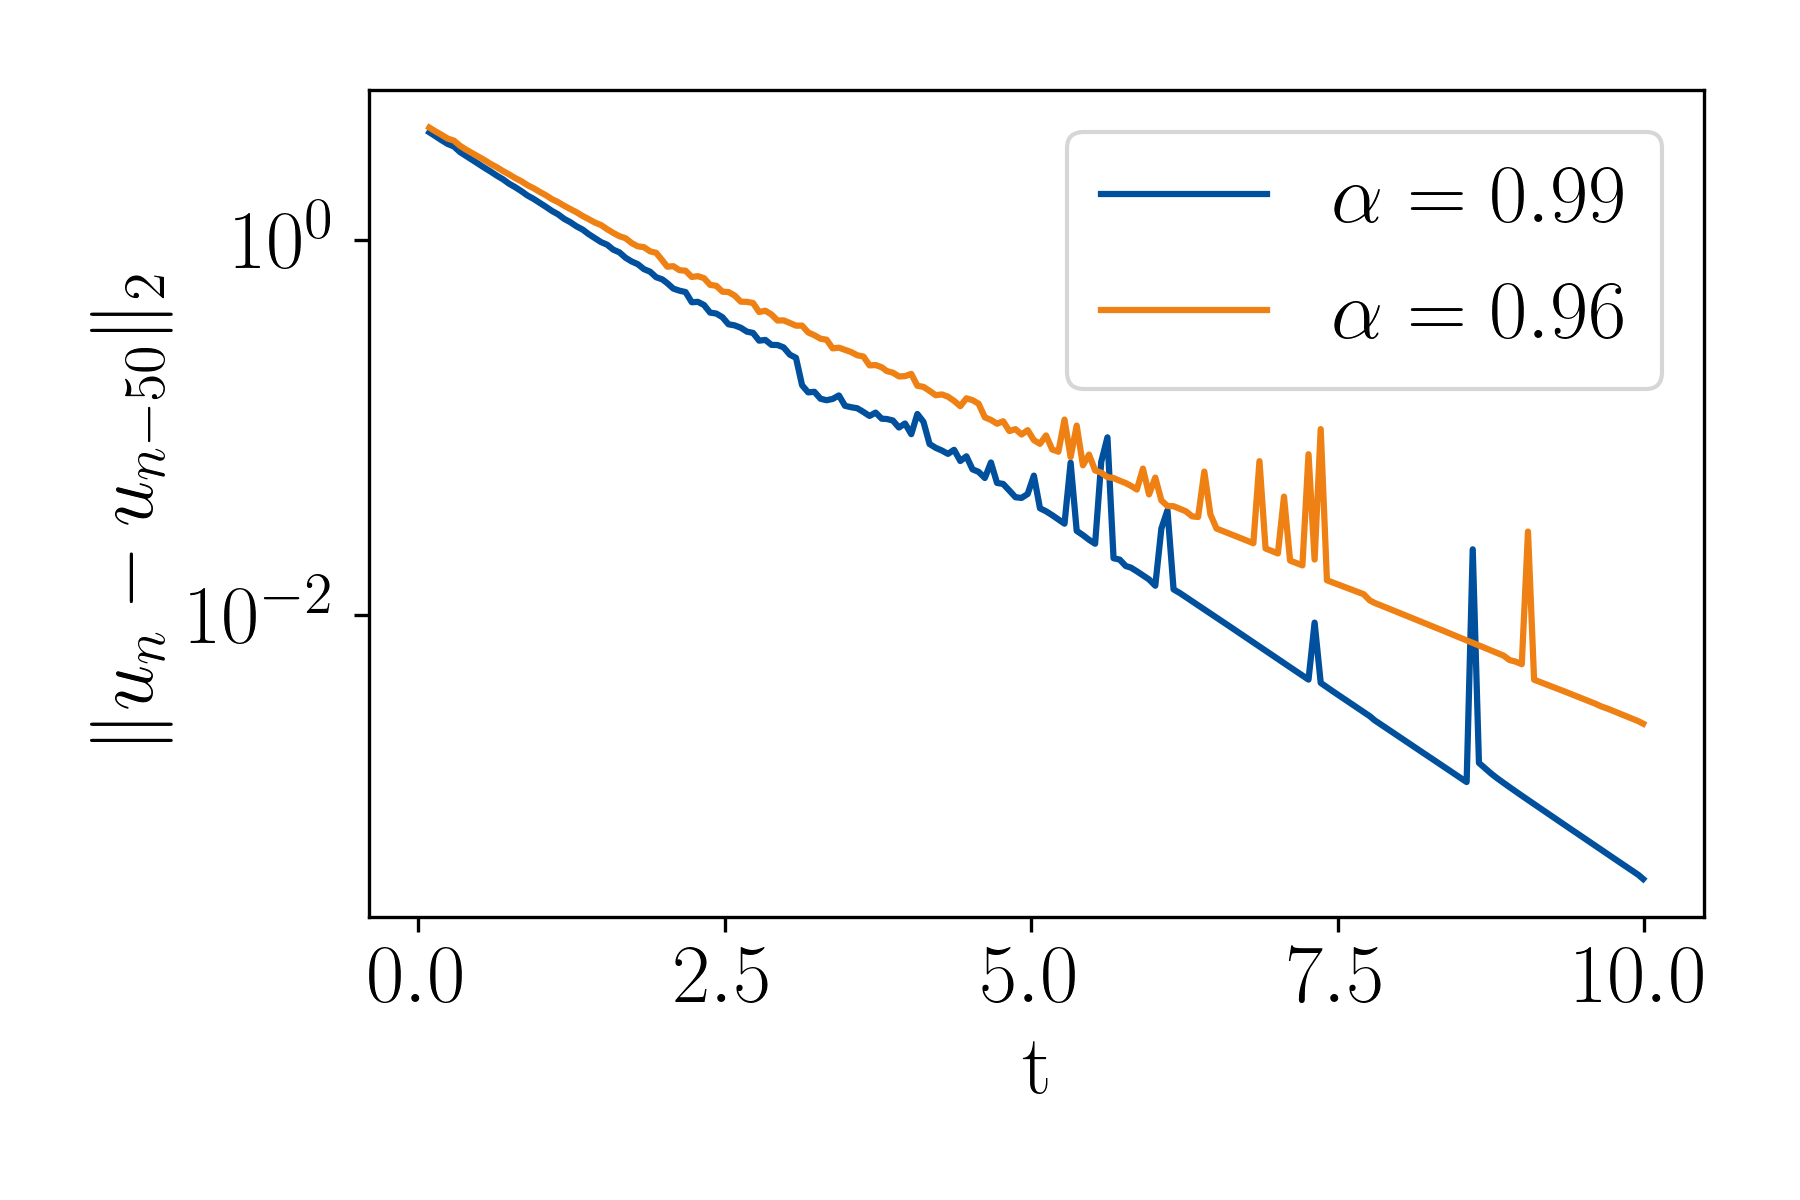
\includegraphics[height=3.5cm]{figures/Results/Circle/model1/99_and_96_res.png}%
}
\end{center}
\vspace{-2.5em}
\caption[Model 1 - Circular example $\alpha=0.99$]{Model 1: $h=0.01$, $10$ level curves, $\alpha=0.99$, $dt=1/10h$, $r_0=0.9$, $200$ points. Reinitialized every $50$ iteration}
\label{fig:model1-a99}
\end{figure}

\begin{comment}
\begin{figure}
\begin{subfigure}{\linewidth}
        \centering
        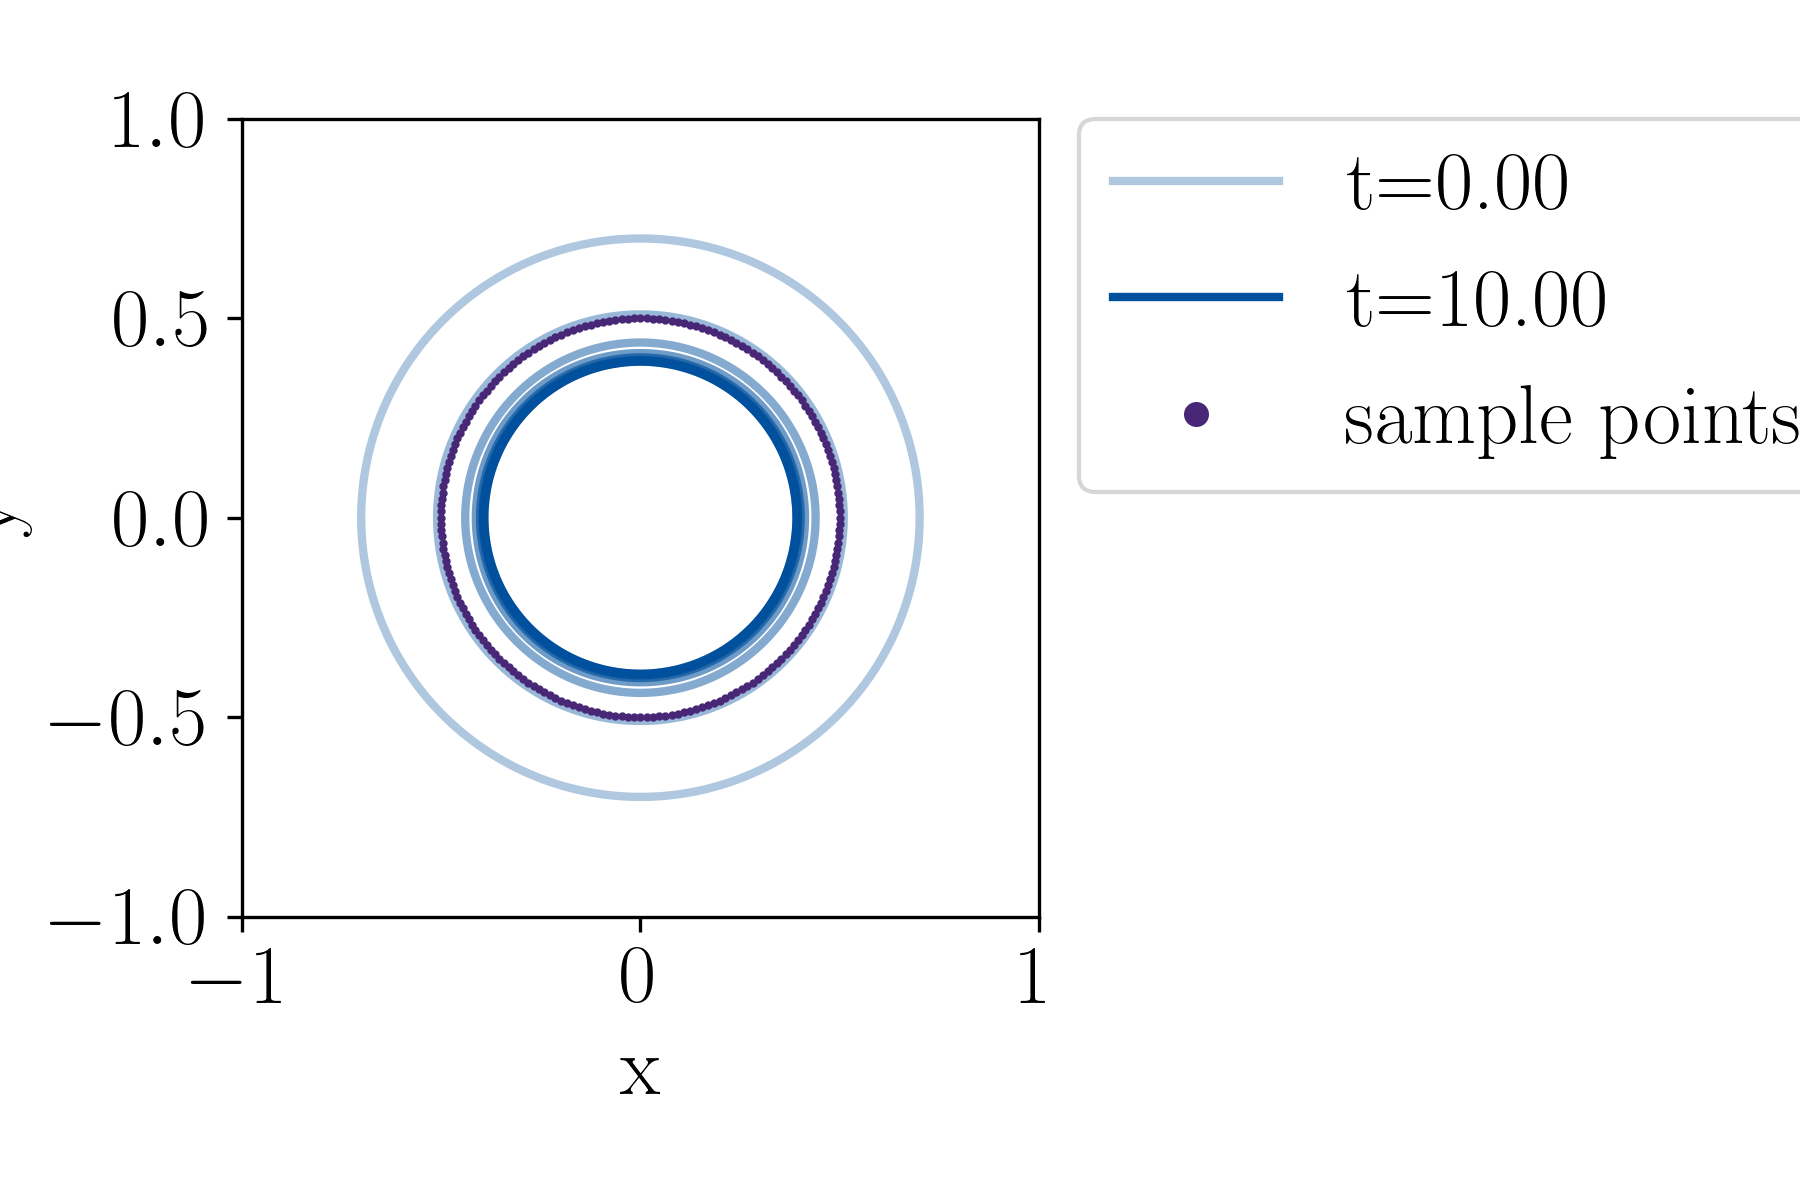
\includegraphics[width=.7\linewidth]{figures/Results/Circle/9-juni/signed-dist/circle-1.png}
        \caption{Caption}
    \end{subfigure} \\[1ex]
    \begin{subfigure}{.5\linewidth}
        \centering
        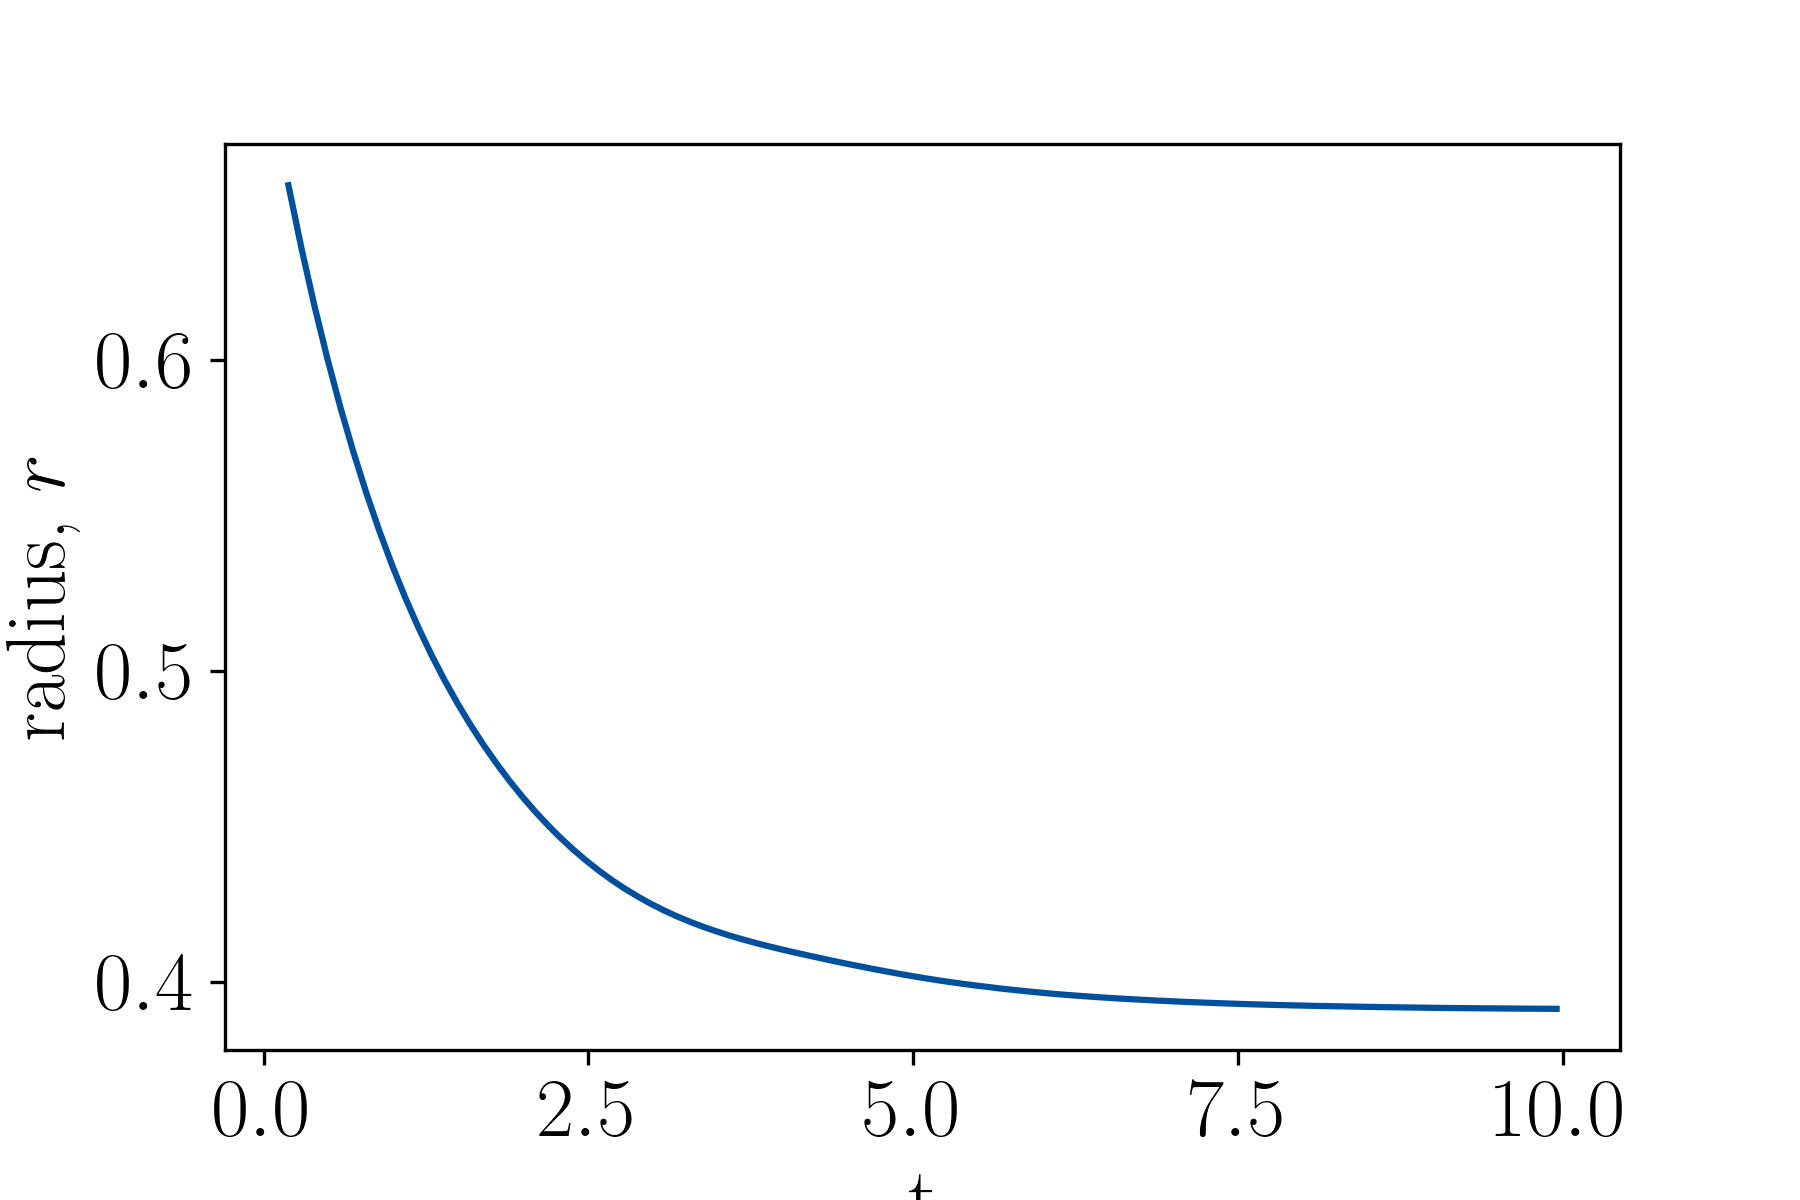
\includegraphics[width=\linewidth]{figures/Results/Circle/9-juni/signed-dist/circle-radius.png}
        \caption{Caption}
        \end{subfigure}%
    \begin{subfigure}{.5\linewidth}
        \centering
        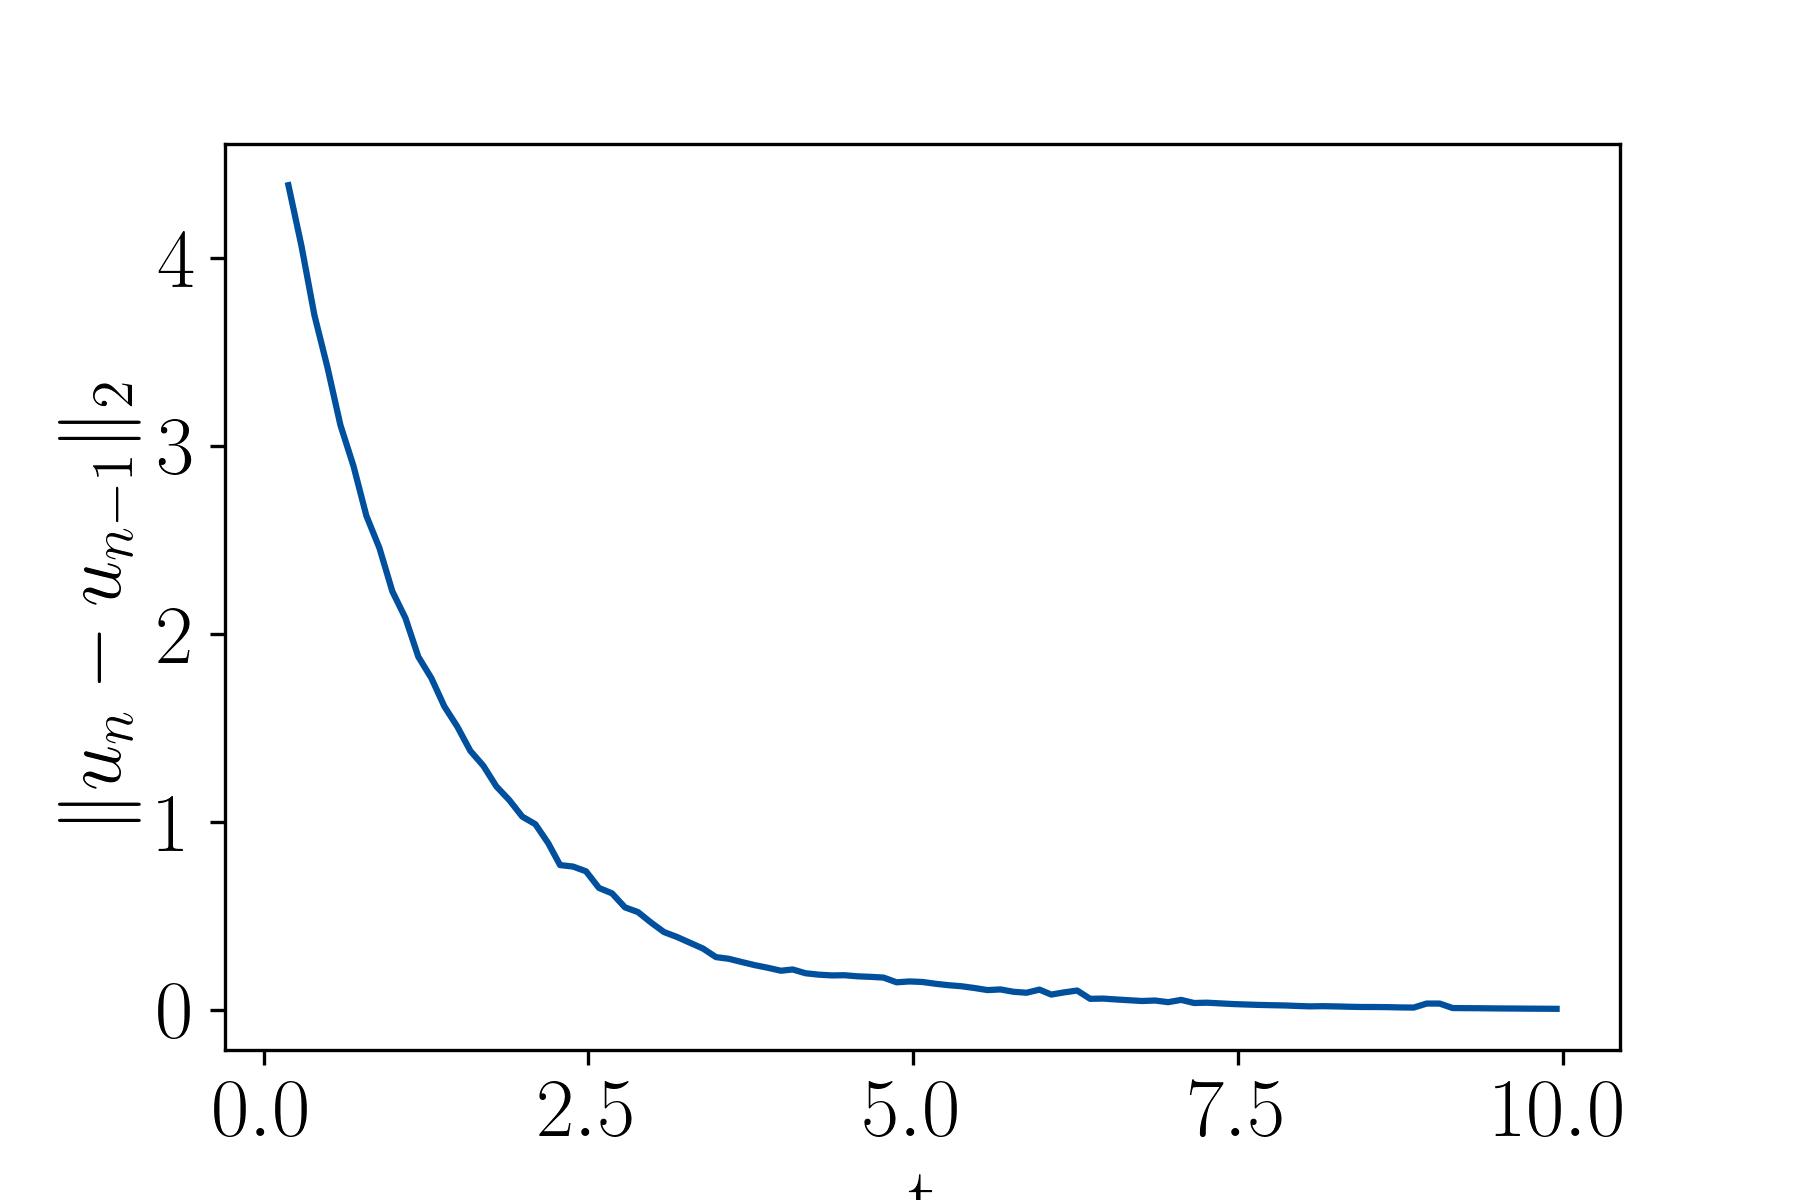
\includegraphics[width=\linewidth]{figures/Results/Circle/9-juni/signed-dist/circle-error.png}
        \caption{Caption}
        \end{subfigure}
    \caption[Model 1 - Curcular Example, Signed Distance]{Model 1: $h=0.01$, $10$ level curves, $\alpha=0.96$, $dt=1/10h$, $r_0=0.7$, $200$ points. Signed distance!! Reinitialized every 100 iteration}
    \label{fig:model1-signed-dist-full}
\end{figure}
\end{comment}

\newpage
Moving over to model 2, we see a big difference in the evolution of the curve compared to model 1. First of all, we see from \figref{fig:m2-circle-radius-numanal} that the numerical solution for model 2 as well follow the evolution of the analytical streamline. Both from this plot and from the residual plot to the right in \figref{fig:model2-circle-a02}, we see that the curve moves the fastest exactly before it reaches $r=r_v=0.5$. This does not come as a surprise, since it follows from the theoretical analysis, but we see that model 2 is not as well suited as model 1 to run a few iterations to get an acceptable answer. 

Furthermore, we see immediately see by looking at the residual plot and the contour plot jointly, that we have an oscillating behavior as was pointed out in the discussion after the theoretical analysis. We see from the residual plot that the velocity do not slow down entirely after hitting the point set, but the curve does not move visibly in the contour plot. The shape of the residual plot, makes this model sensitive for a stopping criterion for this example, seeing that the residual do not decrease under a certain value. Choosing a stopping criterion with too low acceptance may not yield a solution at all.


\begin{figure}
    \centering
    \begin{subfigure}[h]{0.49\textwidth}
        \centering
        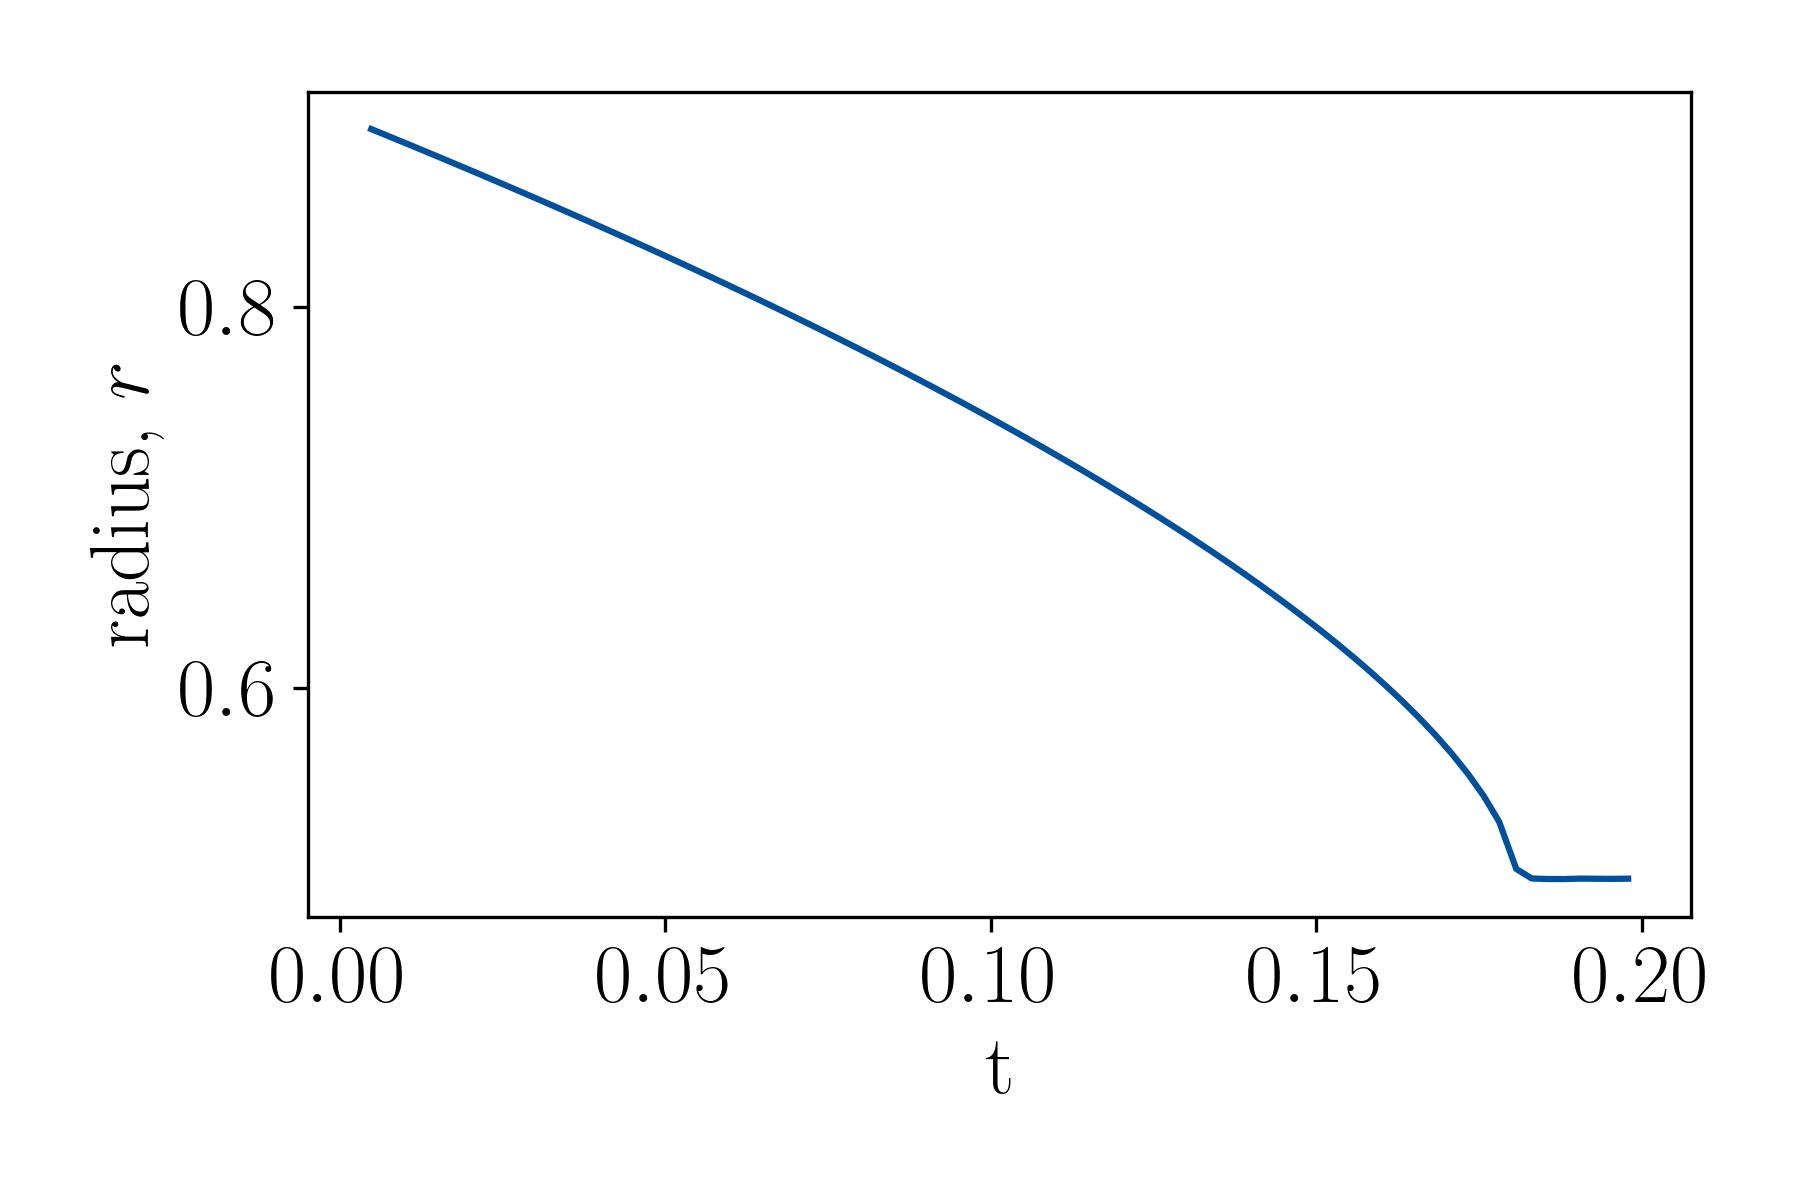
\includegraphics[width=\linewidth]{figures/Results/Circle/model2/circlepoints-a02-rad.png}
        \caption{Numerical solution}
        \label{fig:m2-circle-numerical-radius}
    \end{subfigure}%
    \begin{subfigure}[h]{0.49\textwidth}
        \centering
        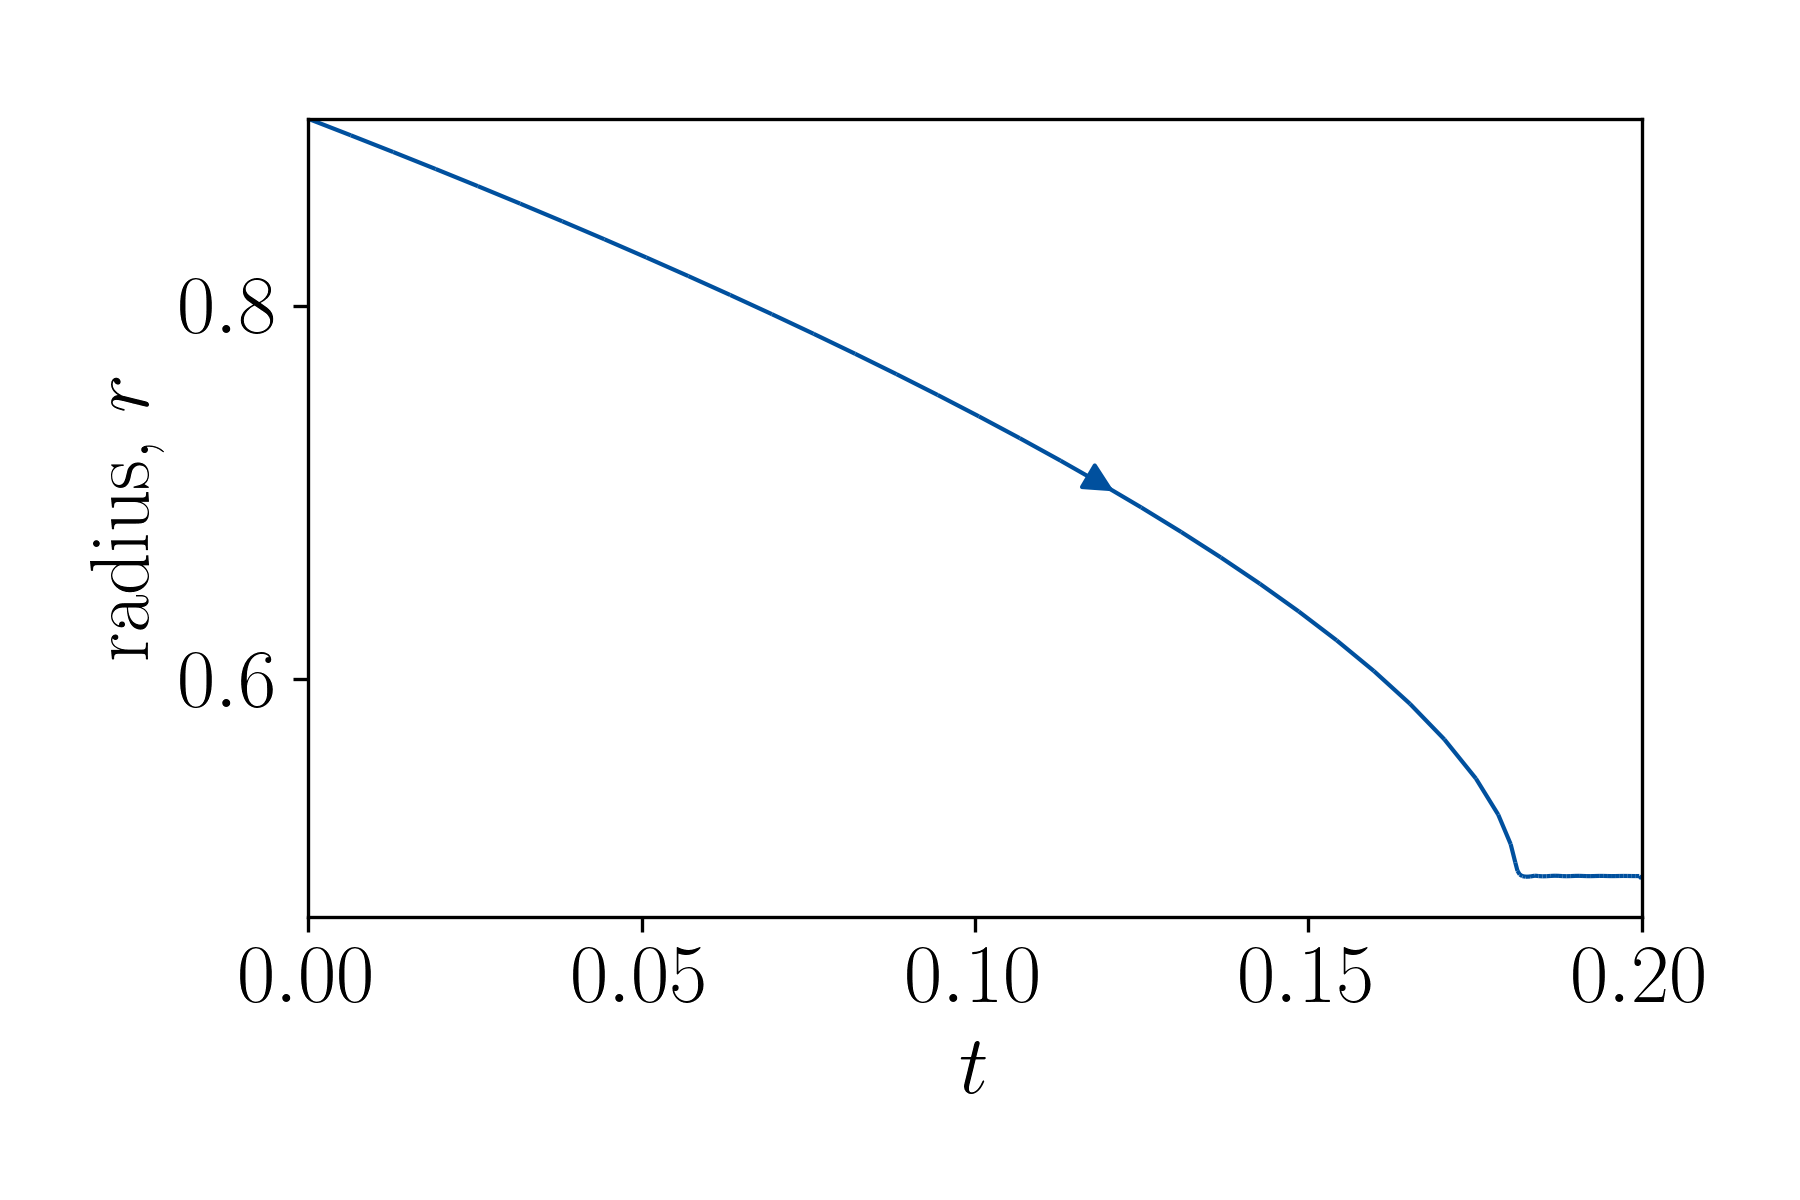
\includegraphics[width=\linewidth]{figures/Circle-radii/mod2-r09.png}
        \caption{Analytical streamline}
        \label{fig:m2-circle-analytical-radius}
    \end{subfigure}
    \caption[Model 2 - Circle, Radius]{The radius over time for the numerical implementation of model 2 on a point set of $200$ points in a circle with radius $0.5$, $\alpha=0.2$, $\delta=10^{-2}$ to the left and the analytical streamline of \eqref{eq:pde-streamline-inverse-1} -- \eqref{eq:pde-streamline-inverse-2} obtained from the analysis of the circular problem with infinitely many sample points with radius $0.5$ to the right. Both the analytical streamline and the numerical solution starts with an initial curve in $r_0=0.9$.}
    \label{fig:m2-circle-radius-numanal}
\end{figure}

\begin{figure}
    \begin{center}
    \resizebox{.99\textwidth}{!}{%
    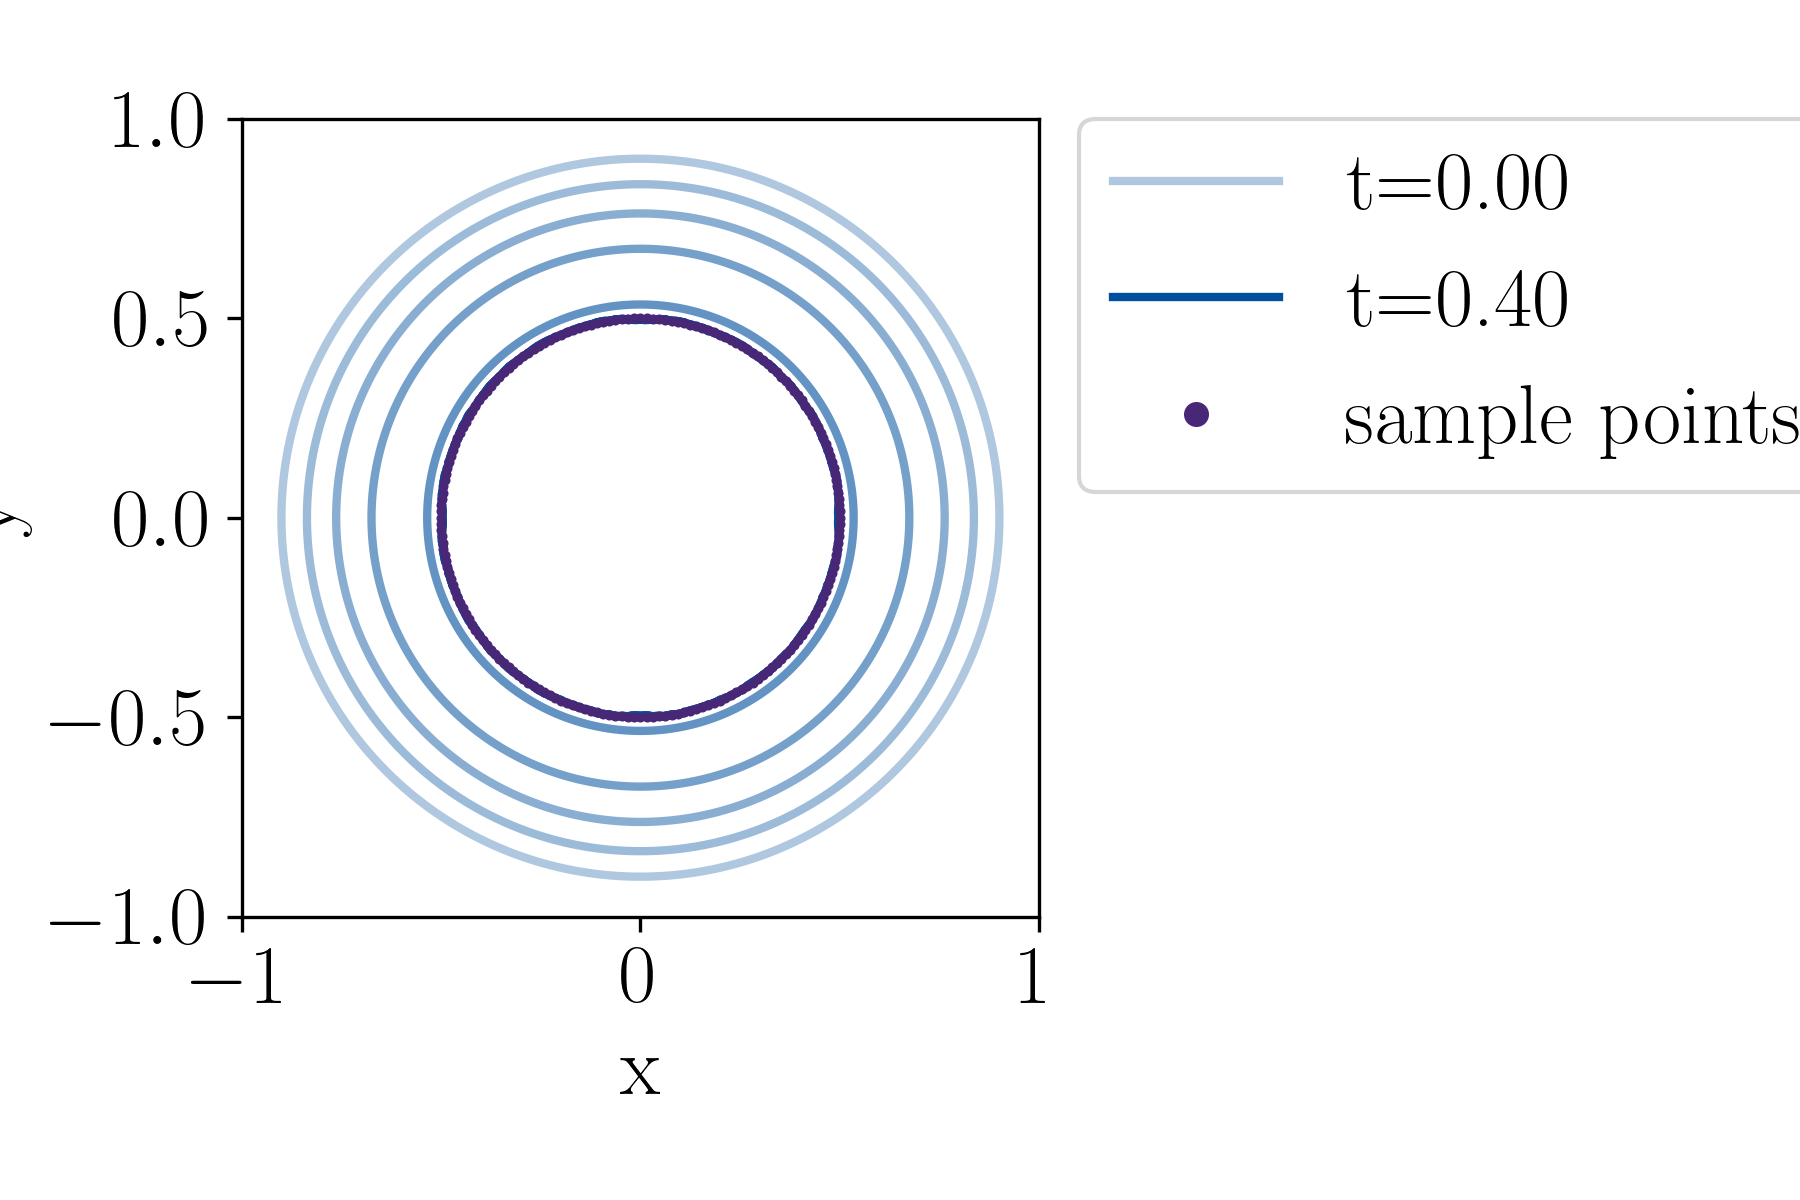
\includegraphics[height=3.5cm]{figures/Results/Circle/model2/circle-a02.png}%
    \,
    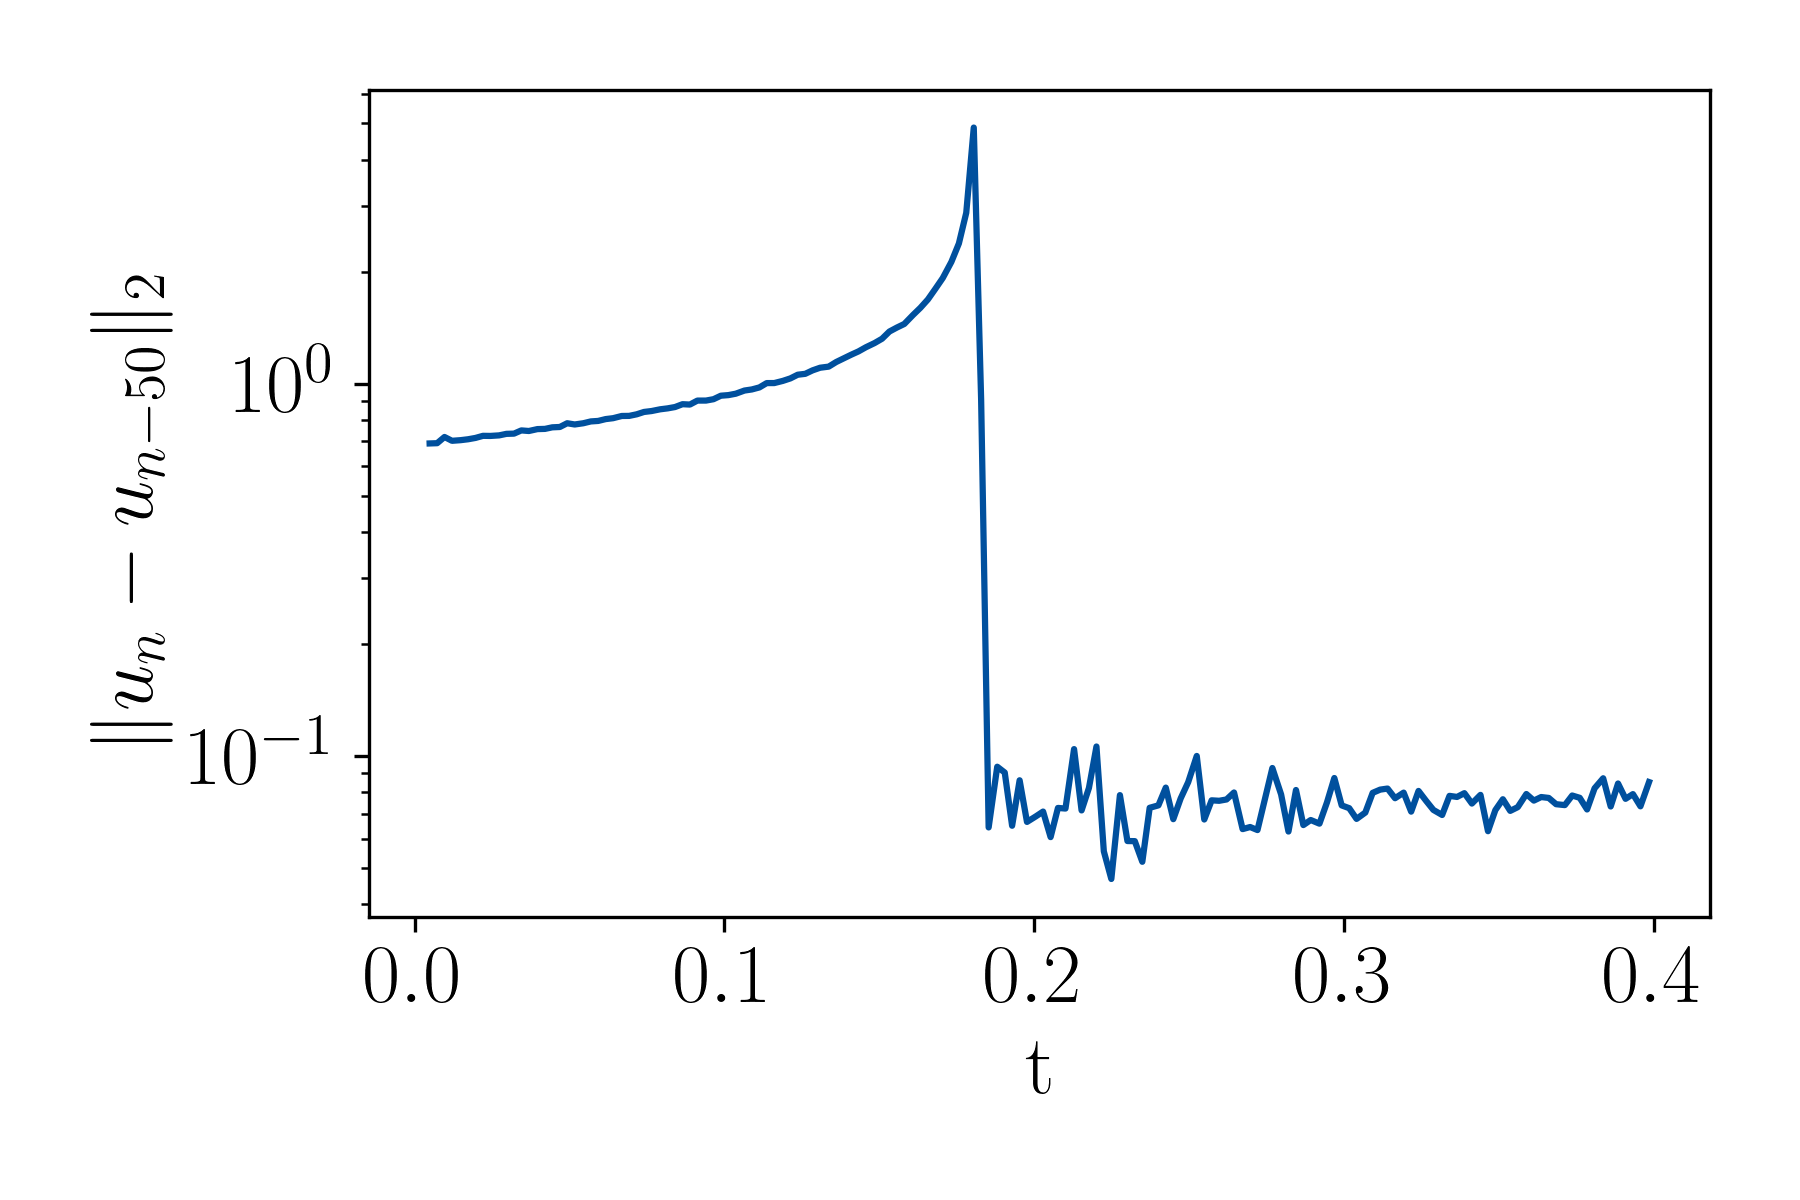
\includegraphics[height=3.5cm]{figures/Results/Circle/model2/circle-a02-logy.png}%
    }
    \end{center}
    \vspace{-2.5em}
    \caption[Model 2- Circular example, $\alpha=0.2$]{Model 2: $h=0.01$, $10$ level curves, $\alpha=0.2$, $dt=1/2 h^2$, $r_0=0.9$, $\delta=10^{-2}$, $200$ points. Reinitialized every $50$ iteration}
    \label{fig:model2-circle-a02}
\end{figure}

Considering the large oscillations after the curve has reached the point set, we want to analyze the effect of the parameter $\delta$. It is natural that it has an effect on the solution when the distance $\distanceVm \to 0$, since $\delta$ in that situation will be dominating. We see from \figref{fig:model2-circle-deltas} that the movement up until the curve reaches the point set is more or less the same, but the behavior afterwards is significantly worse. To support this, we run an additional simulation for $\delta=0.1$, and we see a bigger drop in velocity after the point set radius is reached than for $\delta=10^{-2}$ or $\delta=10^{-4}$. For a smaller value of $\delta$, the velocity from the distance term increases and it is thus natural that also the oscillations increases. 

\begin{figure}
    \centering
    \begin{subfigure}[h]{0.49\textwidth}
        \centering
        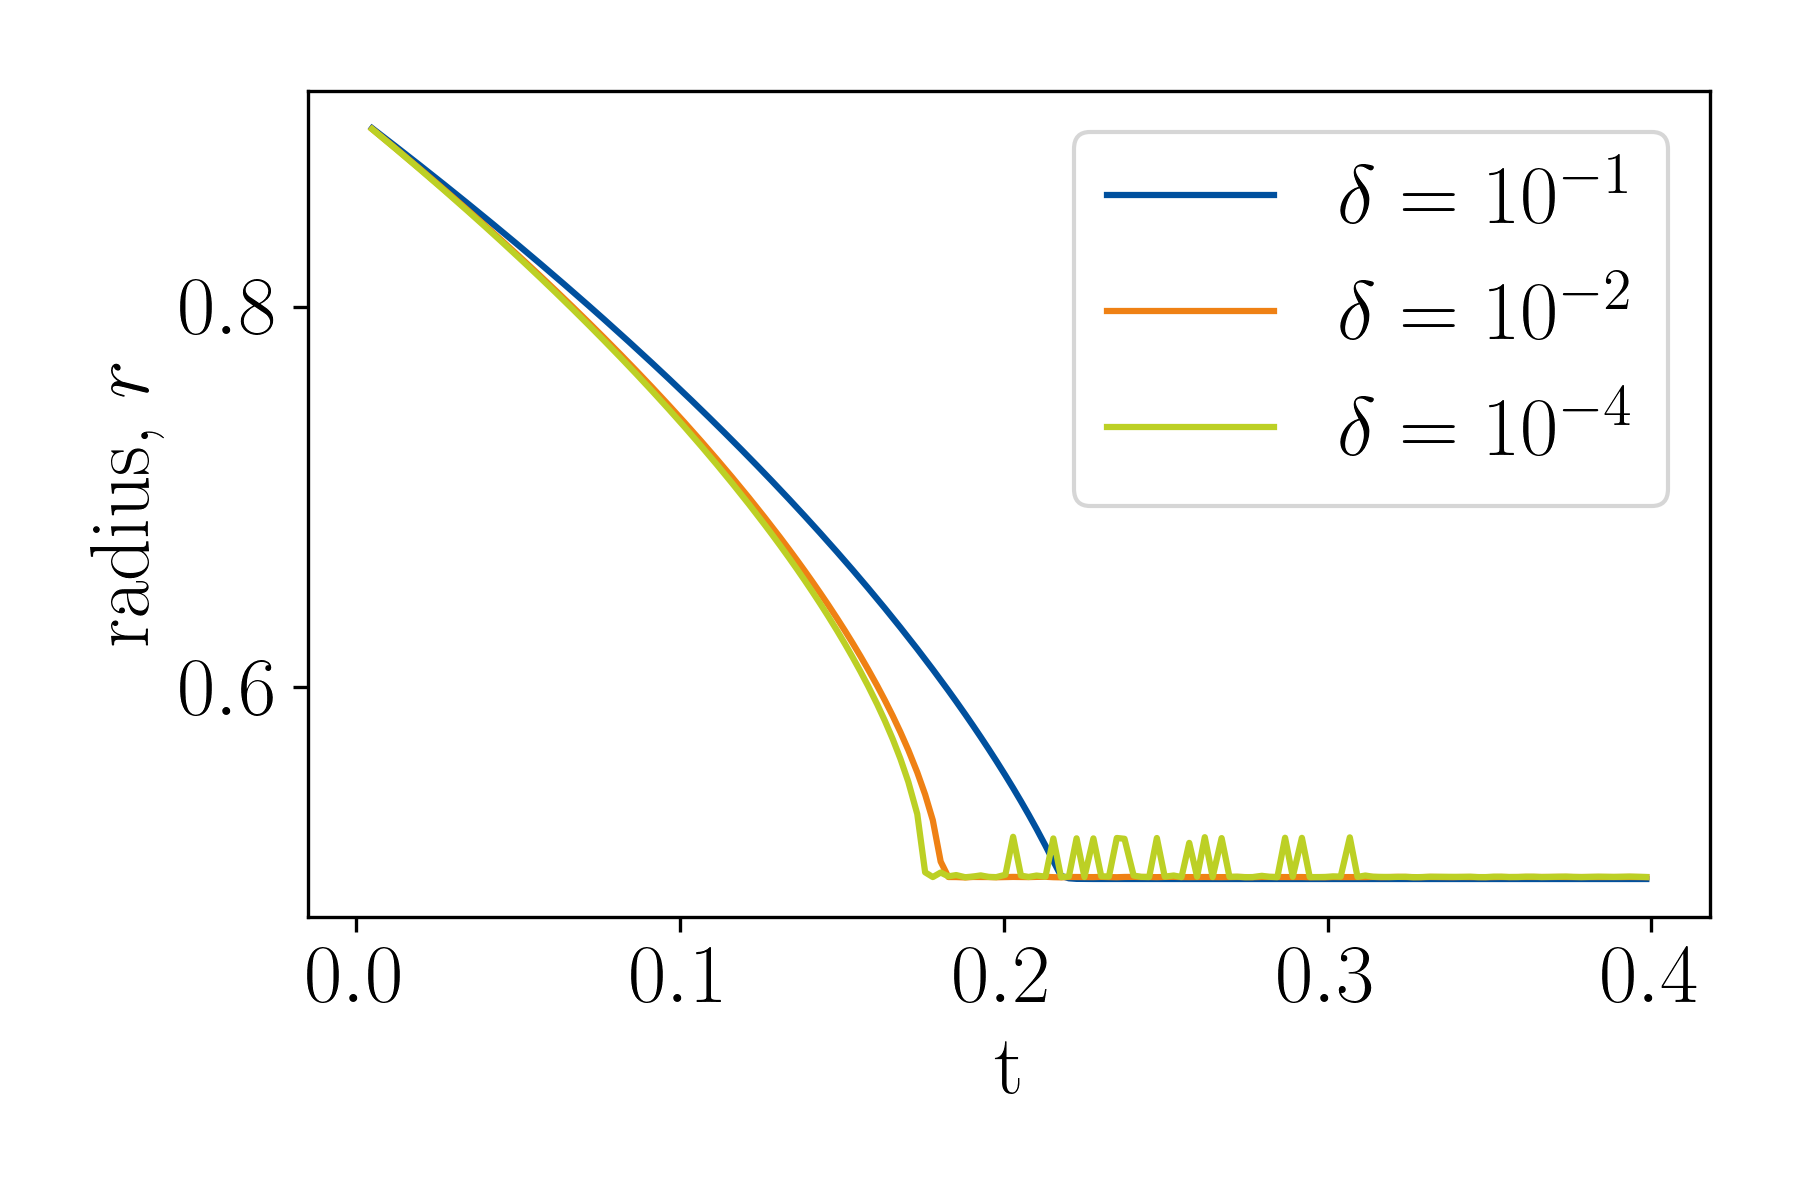
\includegraphics[width=\linewidth]{figures/Results/Circle/model2/d1_d2_d4_rad.png}
    \end{subfigure}%
    \begin{subfigure}[h]{0.49\textwidth}
        \centering
        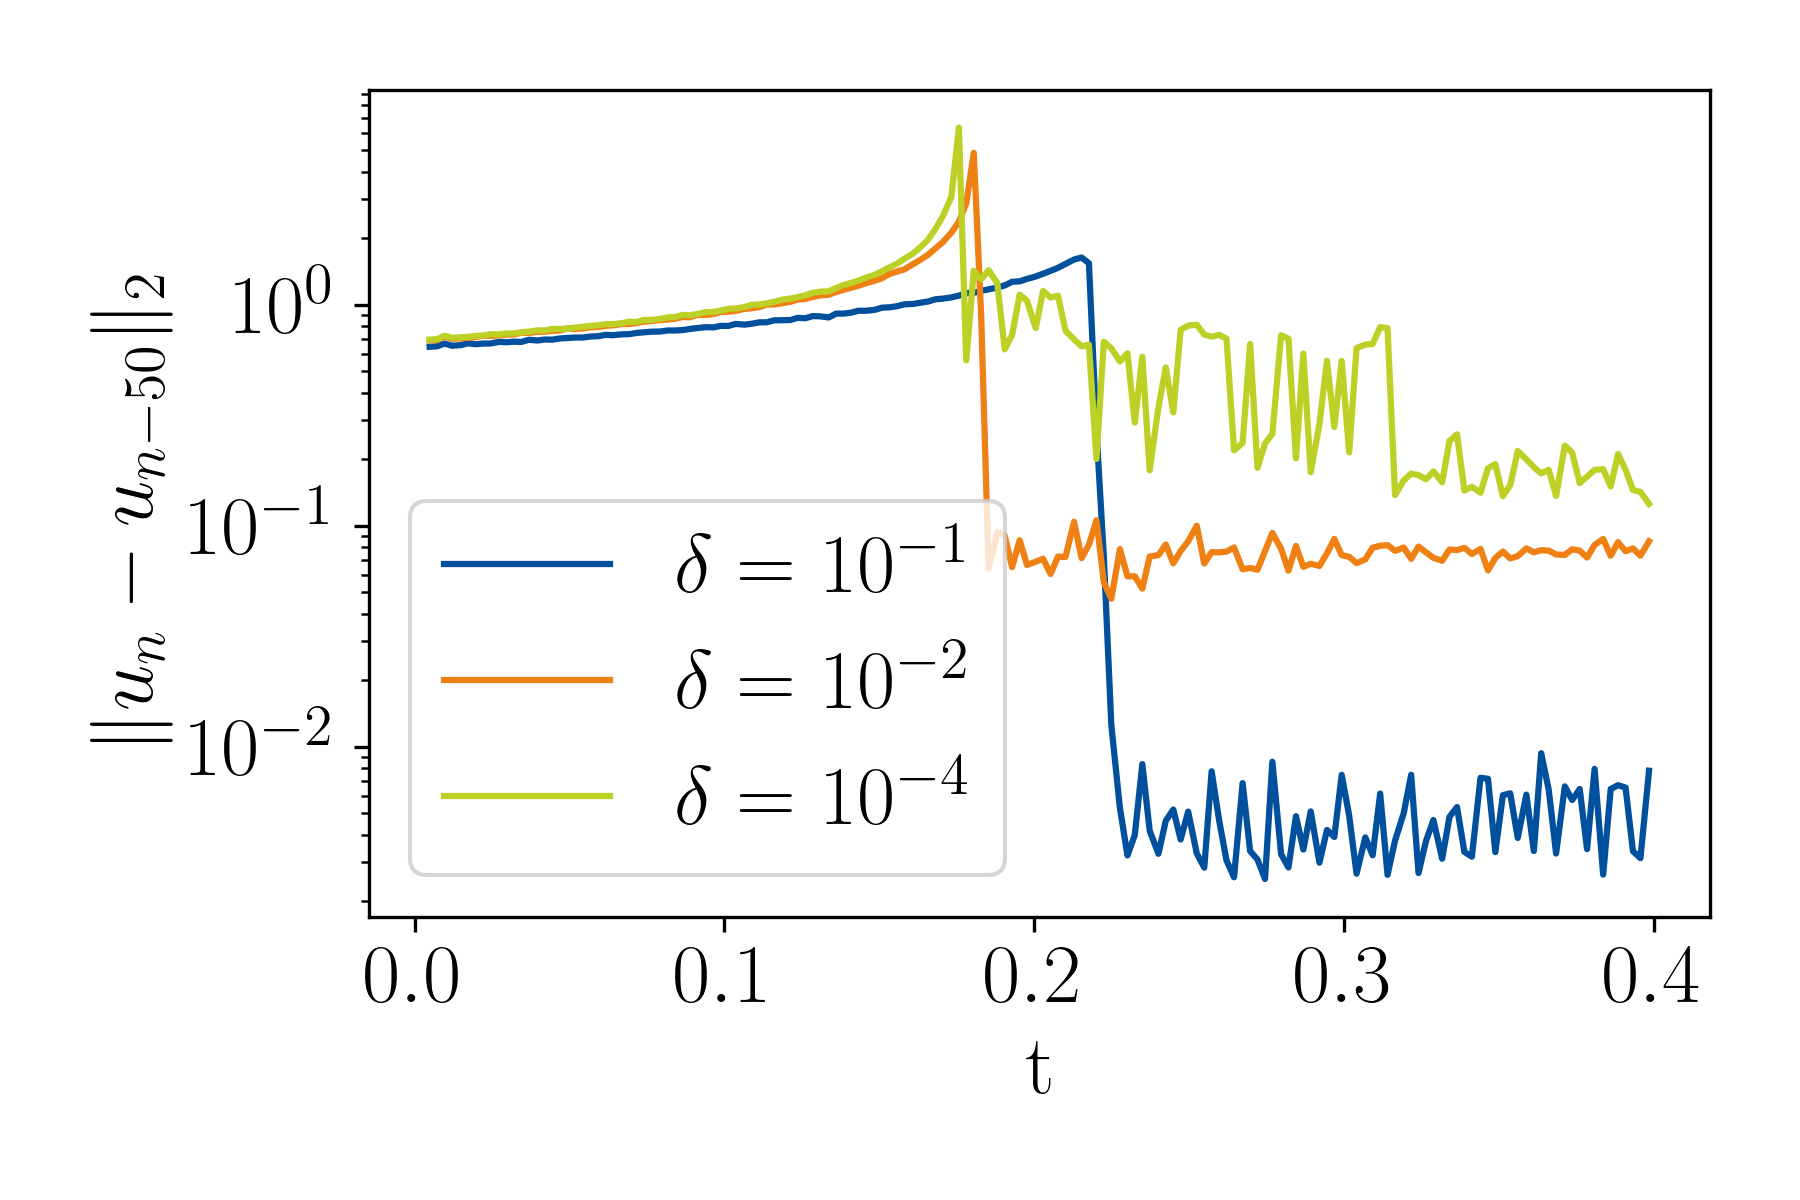
\includegraphics[width=\linewidth]{figures/Results/Circle/model2/d1_d2_d4_res.png}
    \end{subfigure}
    \caption[Model 2 - Circular example, $\delta$ parameter]{Model 2: $h=0.01$, $10$ level curves, $\alpha=0.2$, $dt=1/2 h^2$, $r_0=0.9$, $200$ points. Reinitialized every $50$ iteration}
    \label{fig:model2-circle-deltas}
\end{figure}


We move on to model 3, where there is no $\delta$ parameter. It is as we remembered not needed when we use an $\arctan$-function to bound the distance term when $\distanceVm\to 0$. We run a simulation with the the parameters $\alpha=0.9$ and $\beta=2$ and the evolution of the radius is displayed in \figref{fig:m3-circle-radius-numanal}. Again we find that the numerical curve advances in accordance with the performed analysis which is as we hoped.

\begin{figure}
    \centering
    \begin{subfigure}[h]{0.49\textwidth}
        \centering
        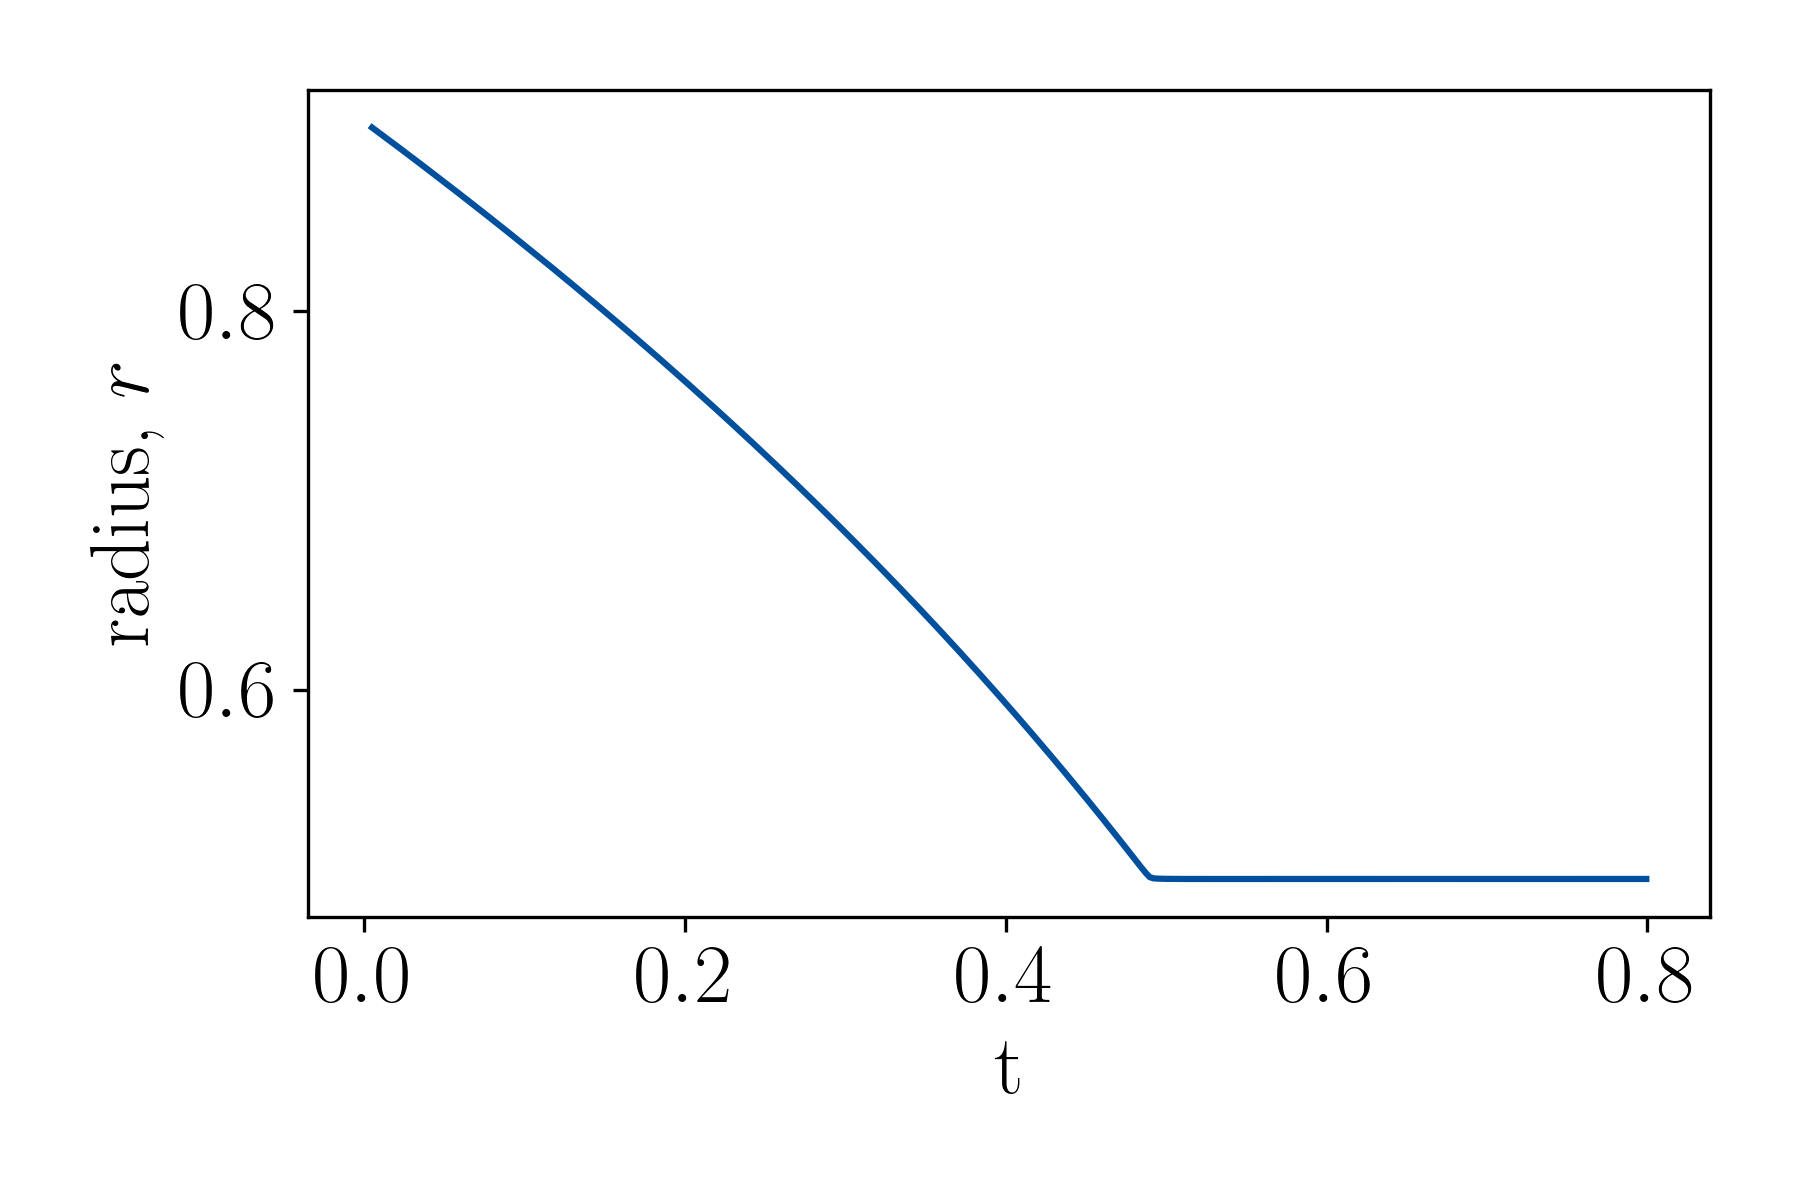
\includegraphics[width=\linewidth]{figures/Results/Circle/model3/circlepoints-a09-rad.png}
        \caption{Numerical solution}
        \label{fig:m3-circle-numerical-radius}
    \end{subfigure}%
    \begin{subfigure}[h]{0.49\textwidth}
        \centering
        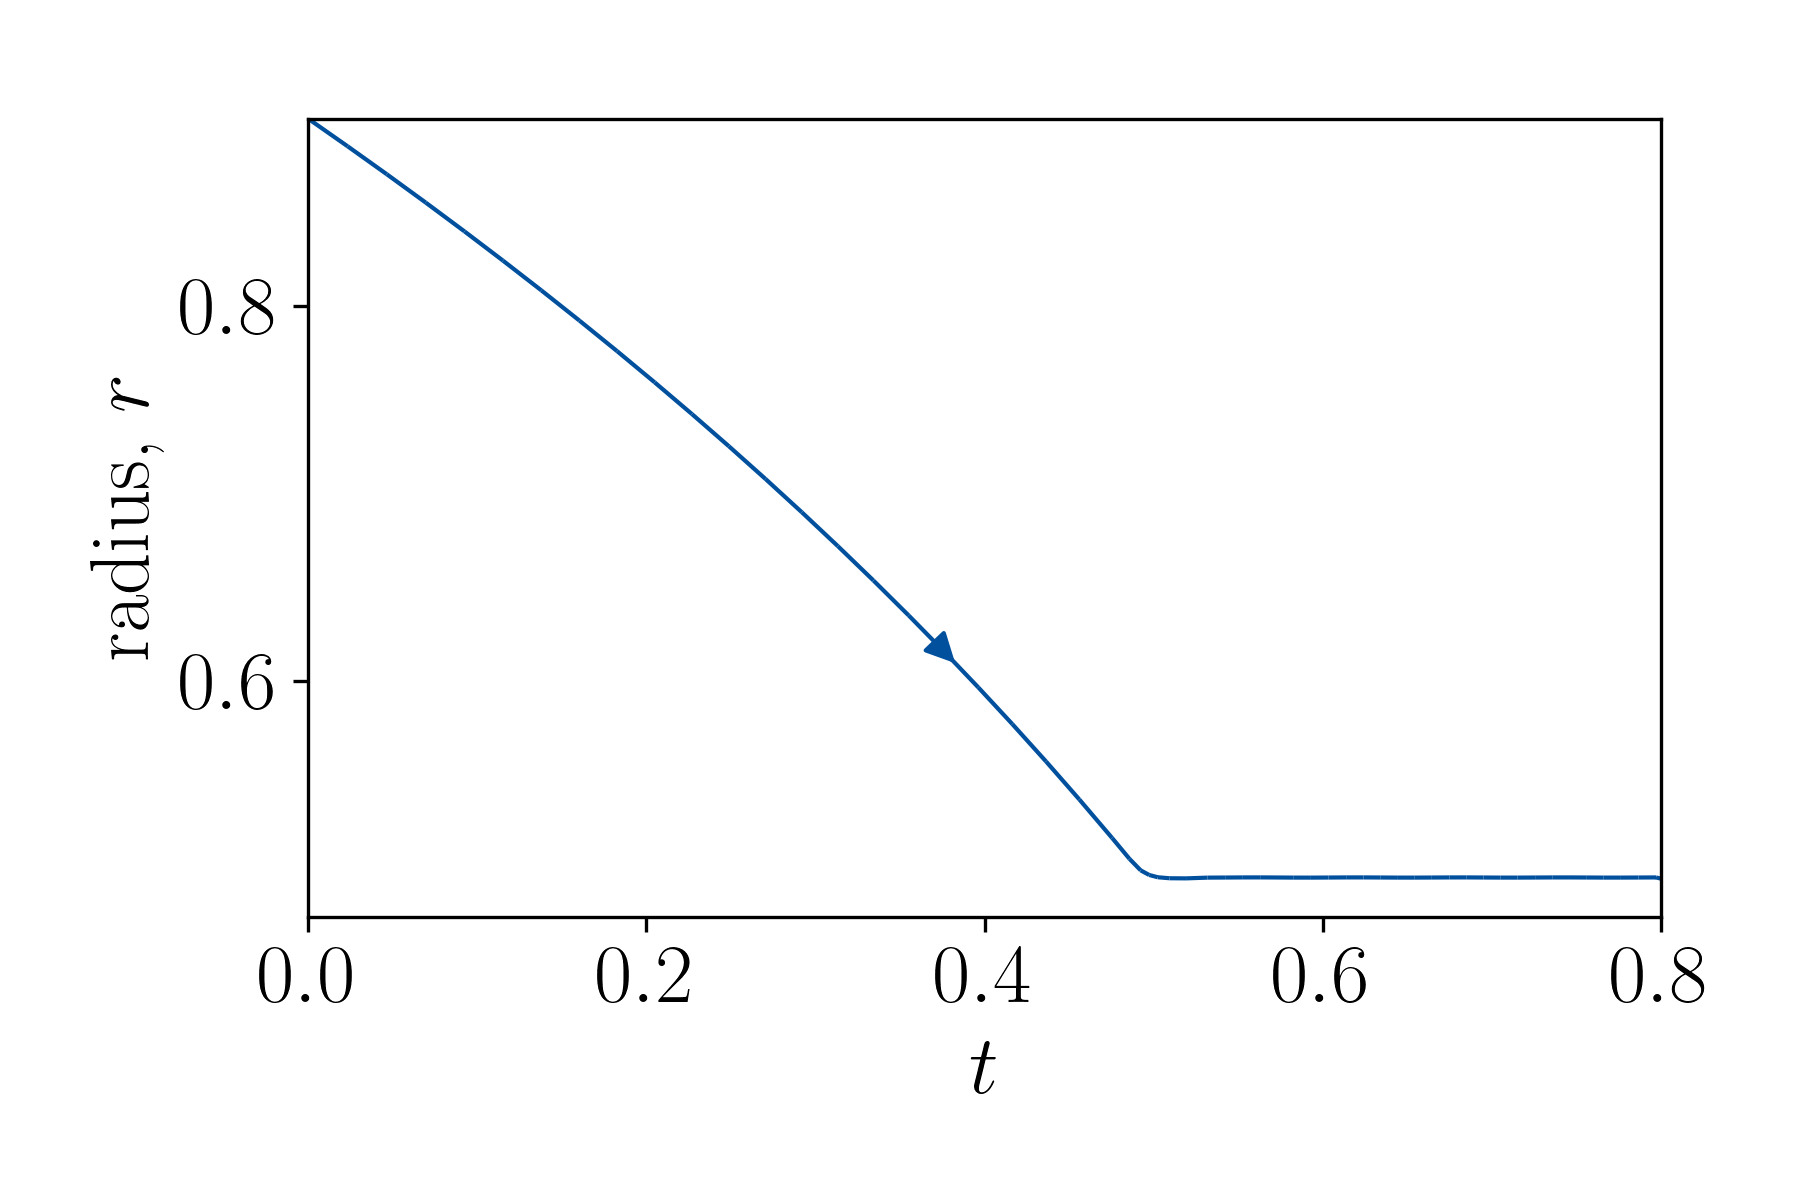
\includegraphics[width=\linewidth]{figures/Circle-radii/mod3-r09.png}
        \caption{Analytical streamline}
        \label{fig:m3-circle-analytical-radius}
    \end{subfigure}
    \caption[Model 3 - Circle, Radius]{The radius over time for the numerical implementation of model 2 on a point set of $200$ points in a circle with radius $0.5$, $\alpha=0.9$, $\beta=2$ to the left and the analytical streamline of \eqref{eq:pde-streamline-inverse-1} -- \eqref{eq:model3-streamline-zero-levelcurve} obtained from the analysis of the circular problem with infinitely many sample points with radius $0.5$ to the right. Both the analytical streamline and the numerical solution starts with an initial curve in $r_0=0.9$.}
    \label{fig:m3-circle-radius-numanal}
\end{figure}

From the residual plot in \figref{fig:model3-circle-a09}, we see that the shape is similar to the residual plot for model 2 with $\delta=0.1$ displayed in \figref{fig:model2-circle-deltas}. This is not unexpected as the speed increases for both models when the distance decreases, and they are both bounded by a constant. For model 2, the shape is more curved up until $t=0.2$ which makes sense because the speed increases exponentially. Since $\delta=0.1$, the exponential growth is cut of at an earlier stage than the plot to the right in \figref{fig:model2-circle-deltas} which has the parameter $\delta=10^{-4}$. The same curved shape is not found in \figref{fig:model3-circle-a09} because $\arctan(1/x)$ is much less steep than $1/x$.

\begin{figure}
    \begin{center}
    \resizebox{.99\textwidth}{!}{%
    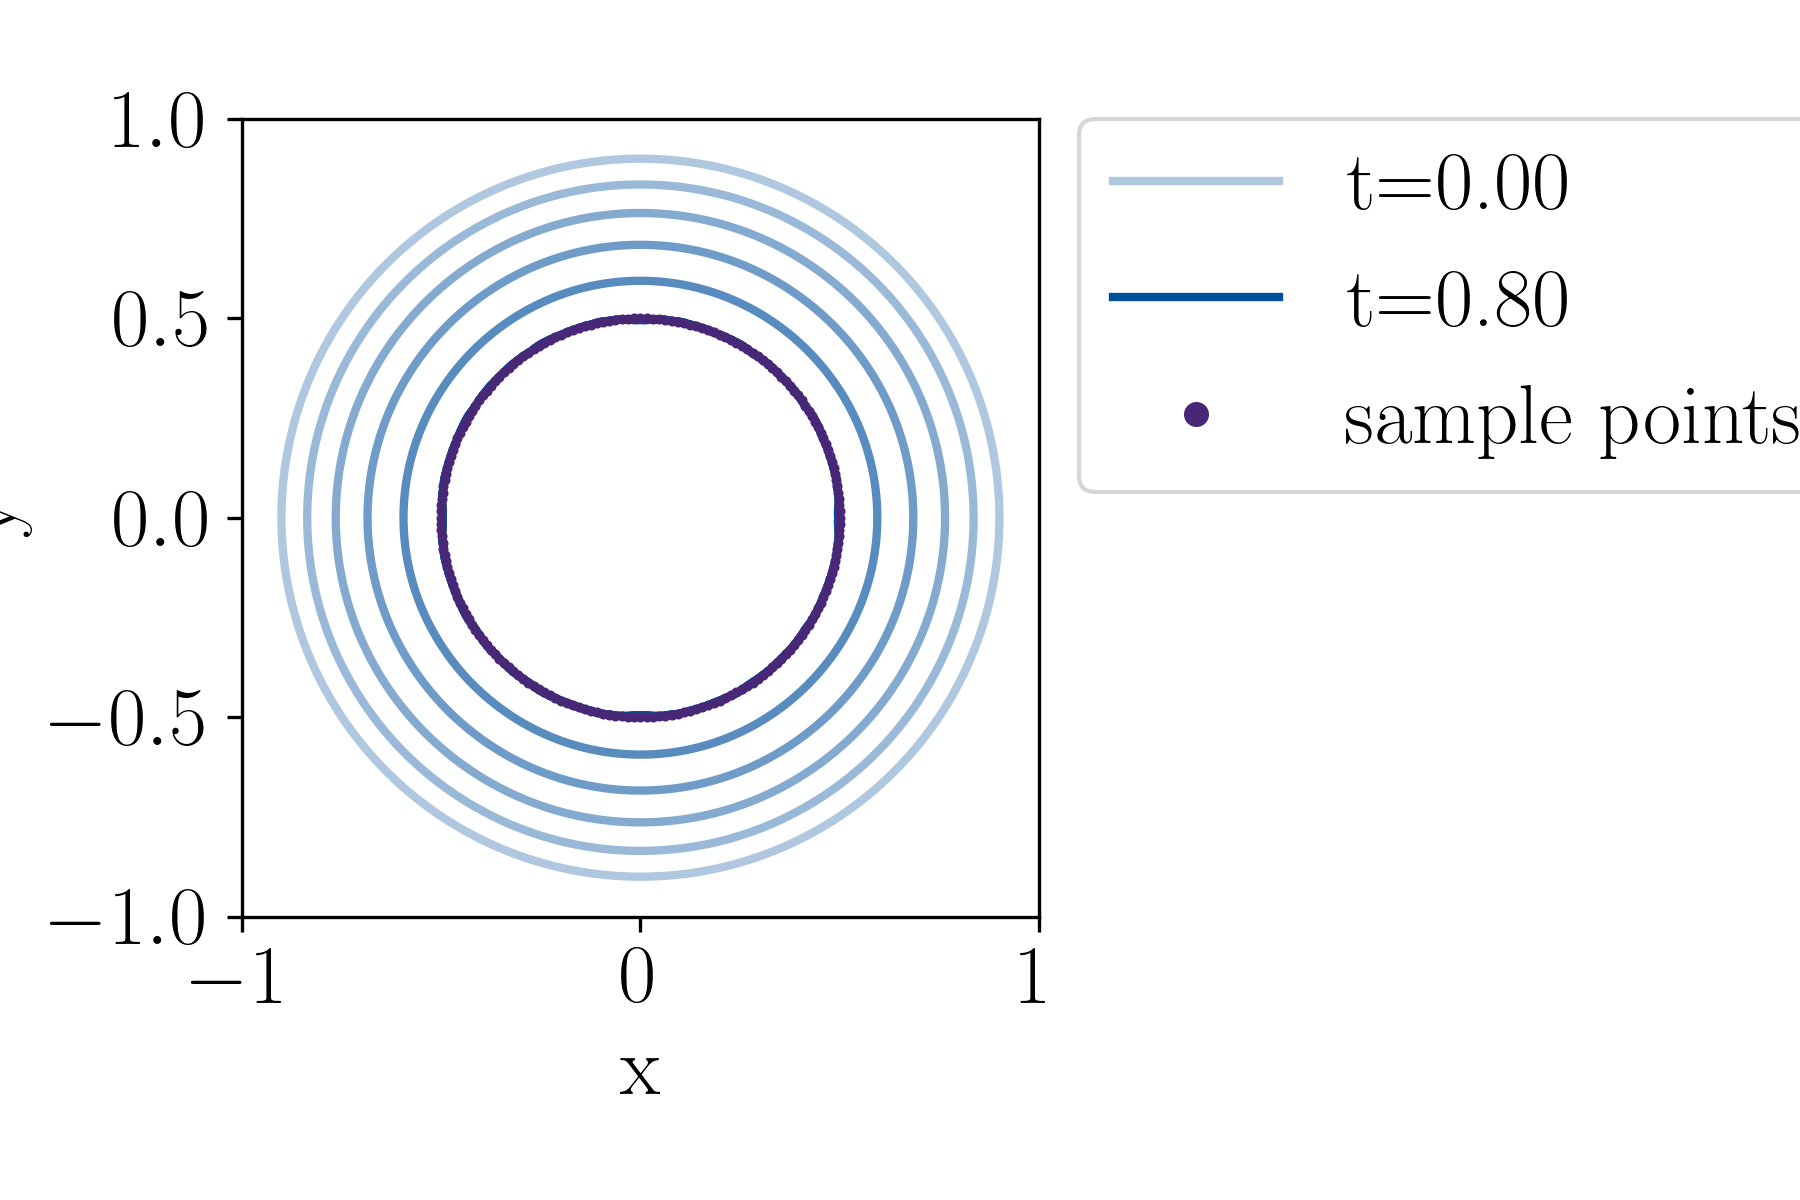
\includegraphics[height=3.5cm]{figures/Results/Circle/model3/circlepoints-a09.png}%
    \,
    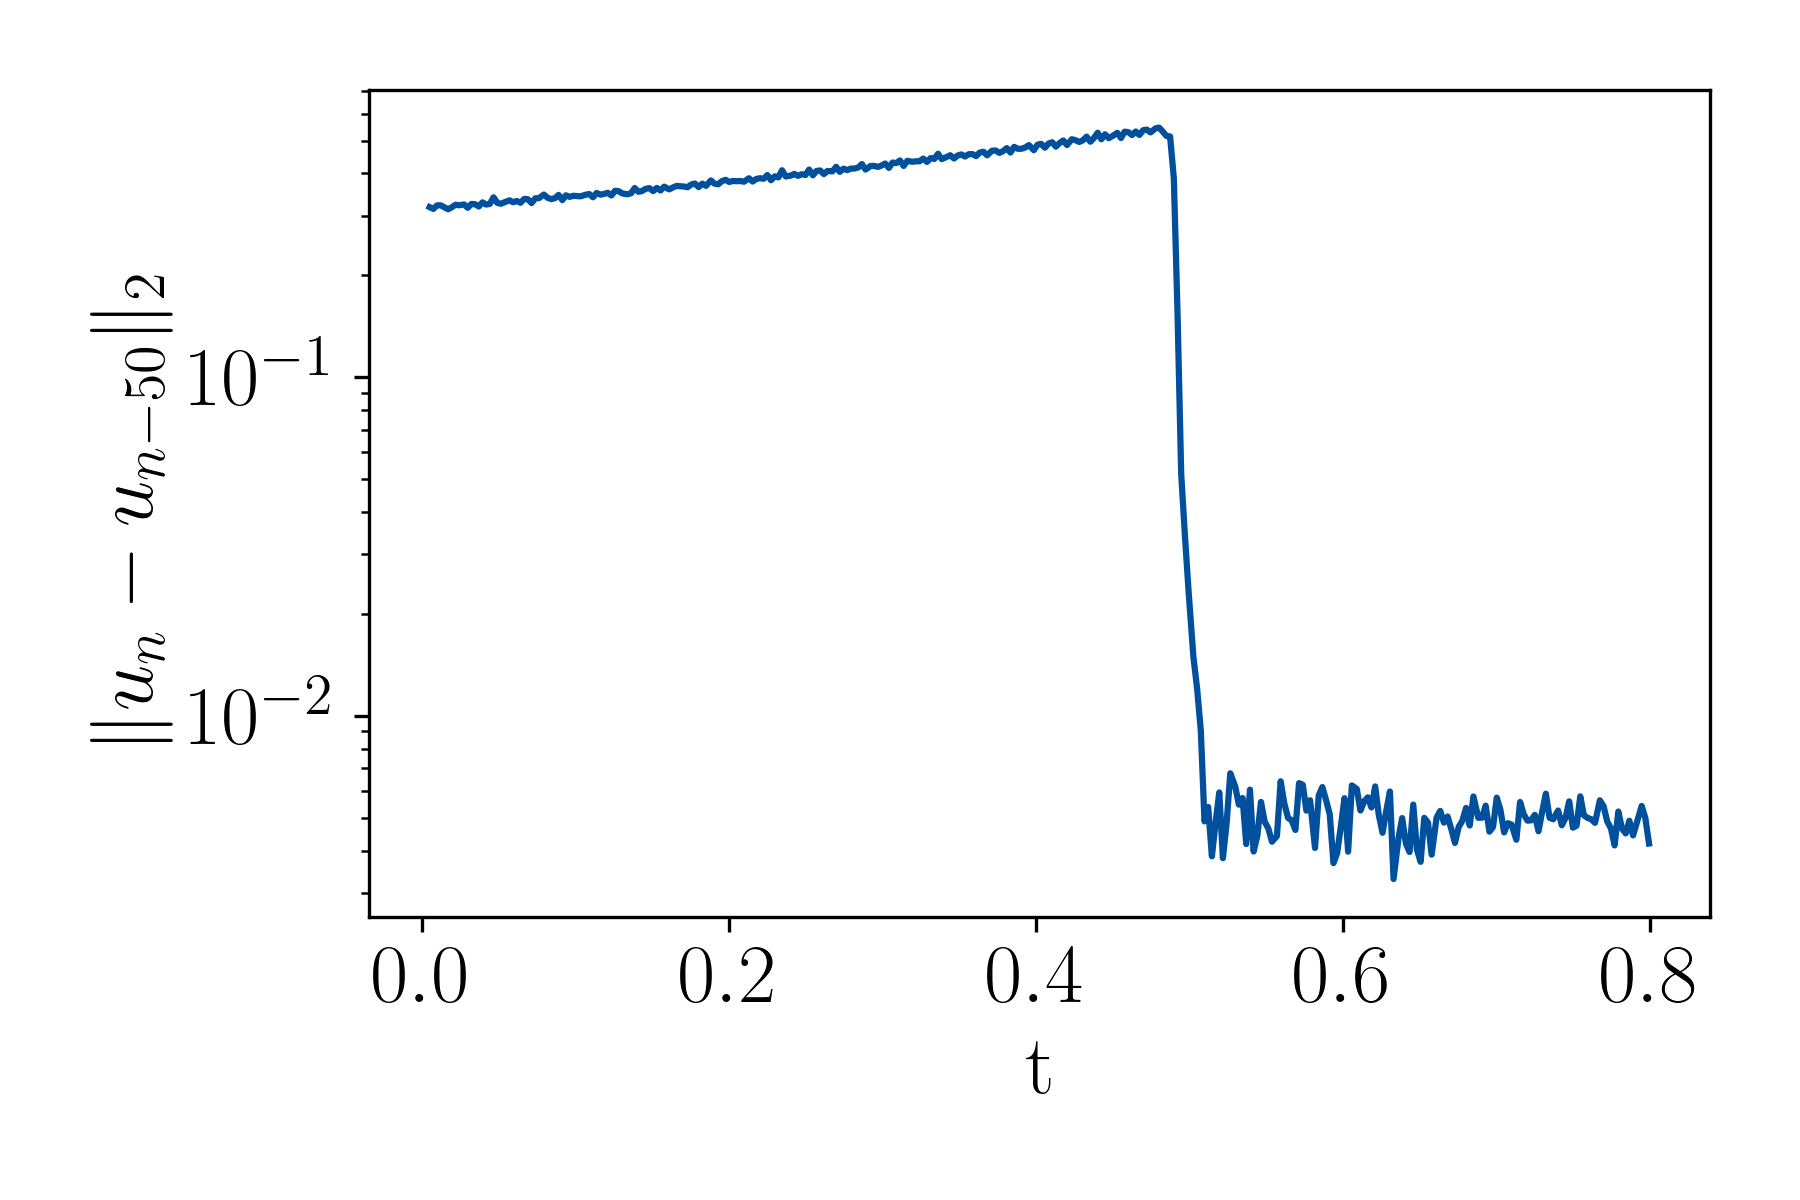
\includegraphics[height=3.5cm]{figures/Results/Circle/model3/circle-a09-b2-logy.png}%
    }
    \end{center}
    \vspace{-2.5em}
    \caption[Model 3 - Circular example, $\alpha=0.9$]{Model 2: $h=0.01$, $10$ level curves, $\alpha=0.9$, $dt=1/2 h^2$, $r_0=0.9$, $\beta=2$, $200$ points. Reinitialized every $50$ iteration}
    \label{fig:model3-circle-a09}
\end{figure}

\begin{figure}
    \centering
    \begin{subfigure}[h]{0.49\textwidth}
        \centering
        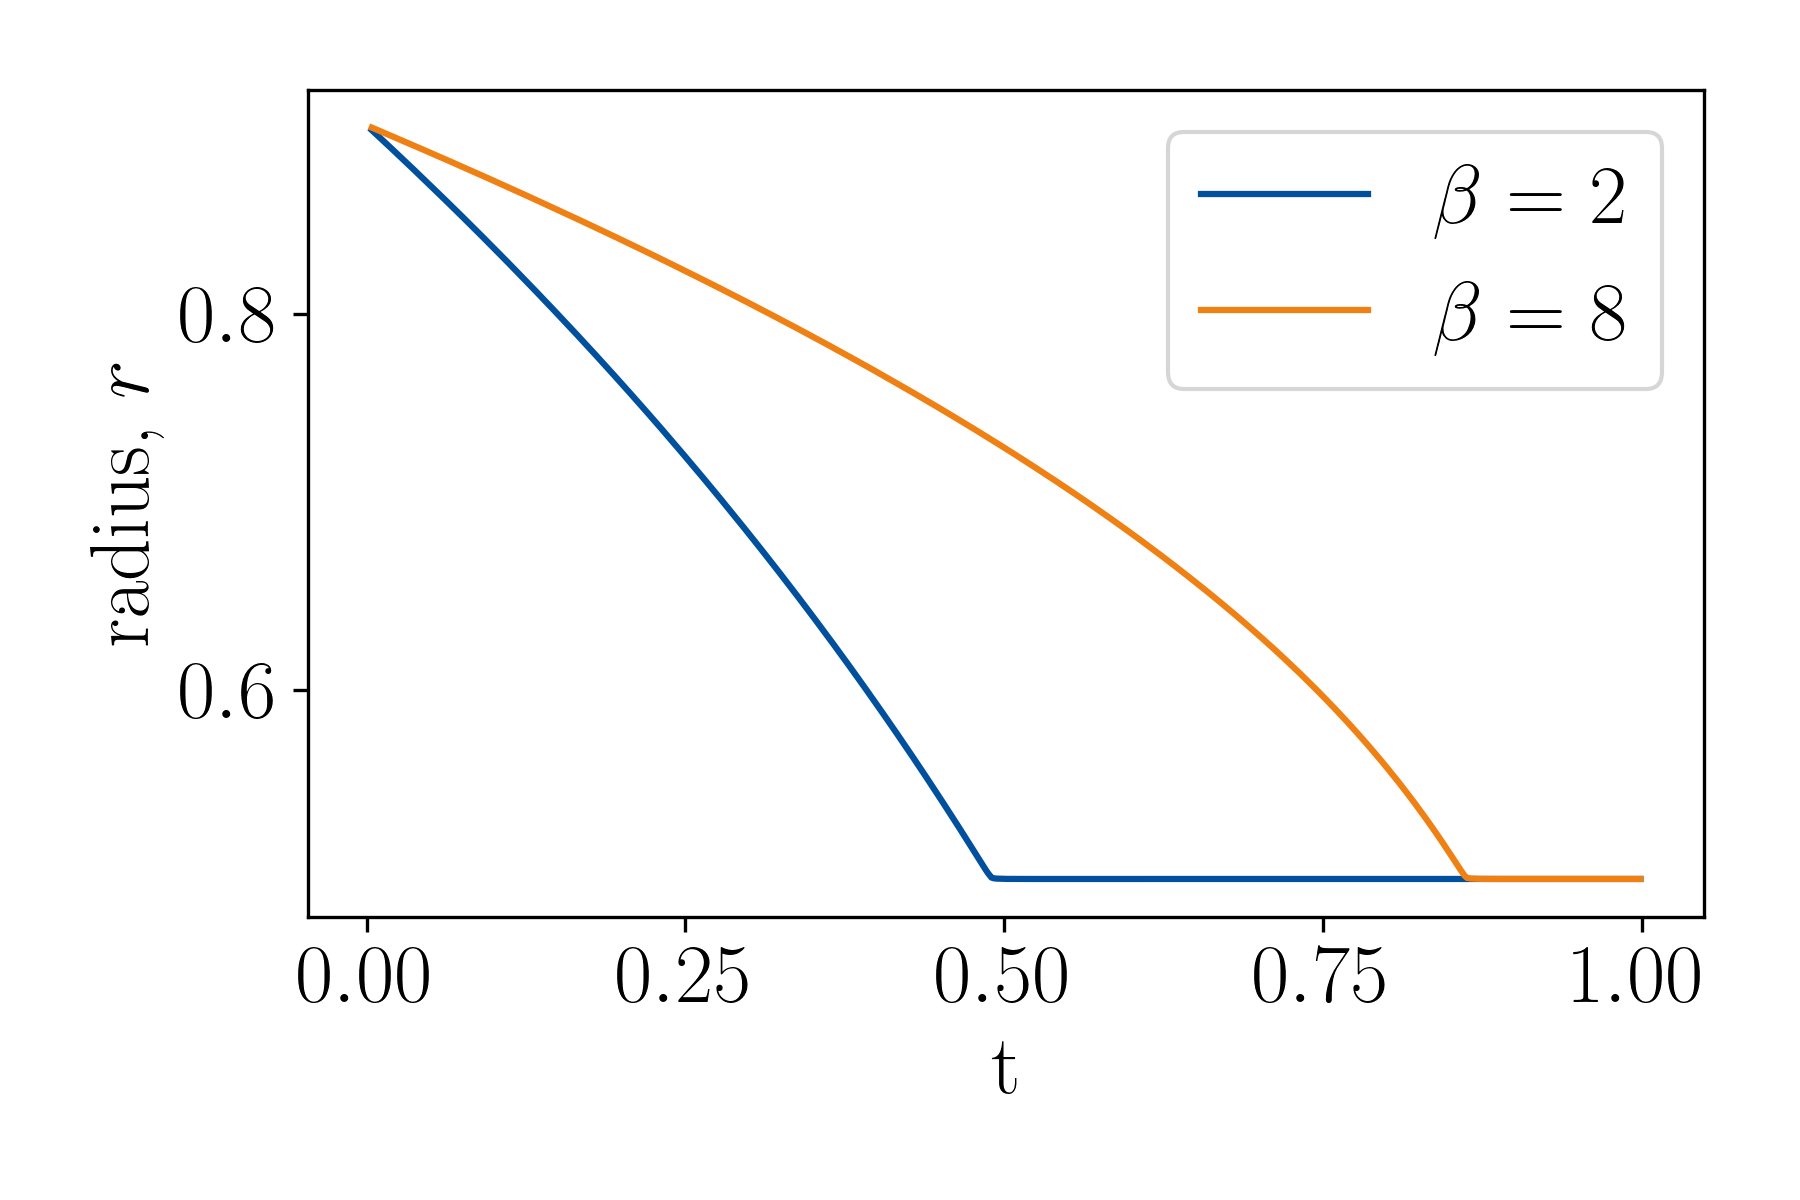
\includegraphics[width=\linewidth]{figures/Results/Circle/model3/b2_b8_rad.png}
    \end{subfigure}%
    \begin{subfigure}[h]{0.49\textwidth}
        \centering
        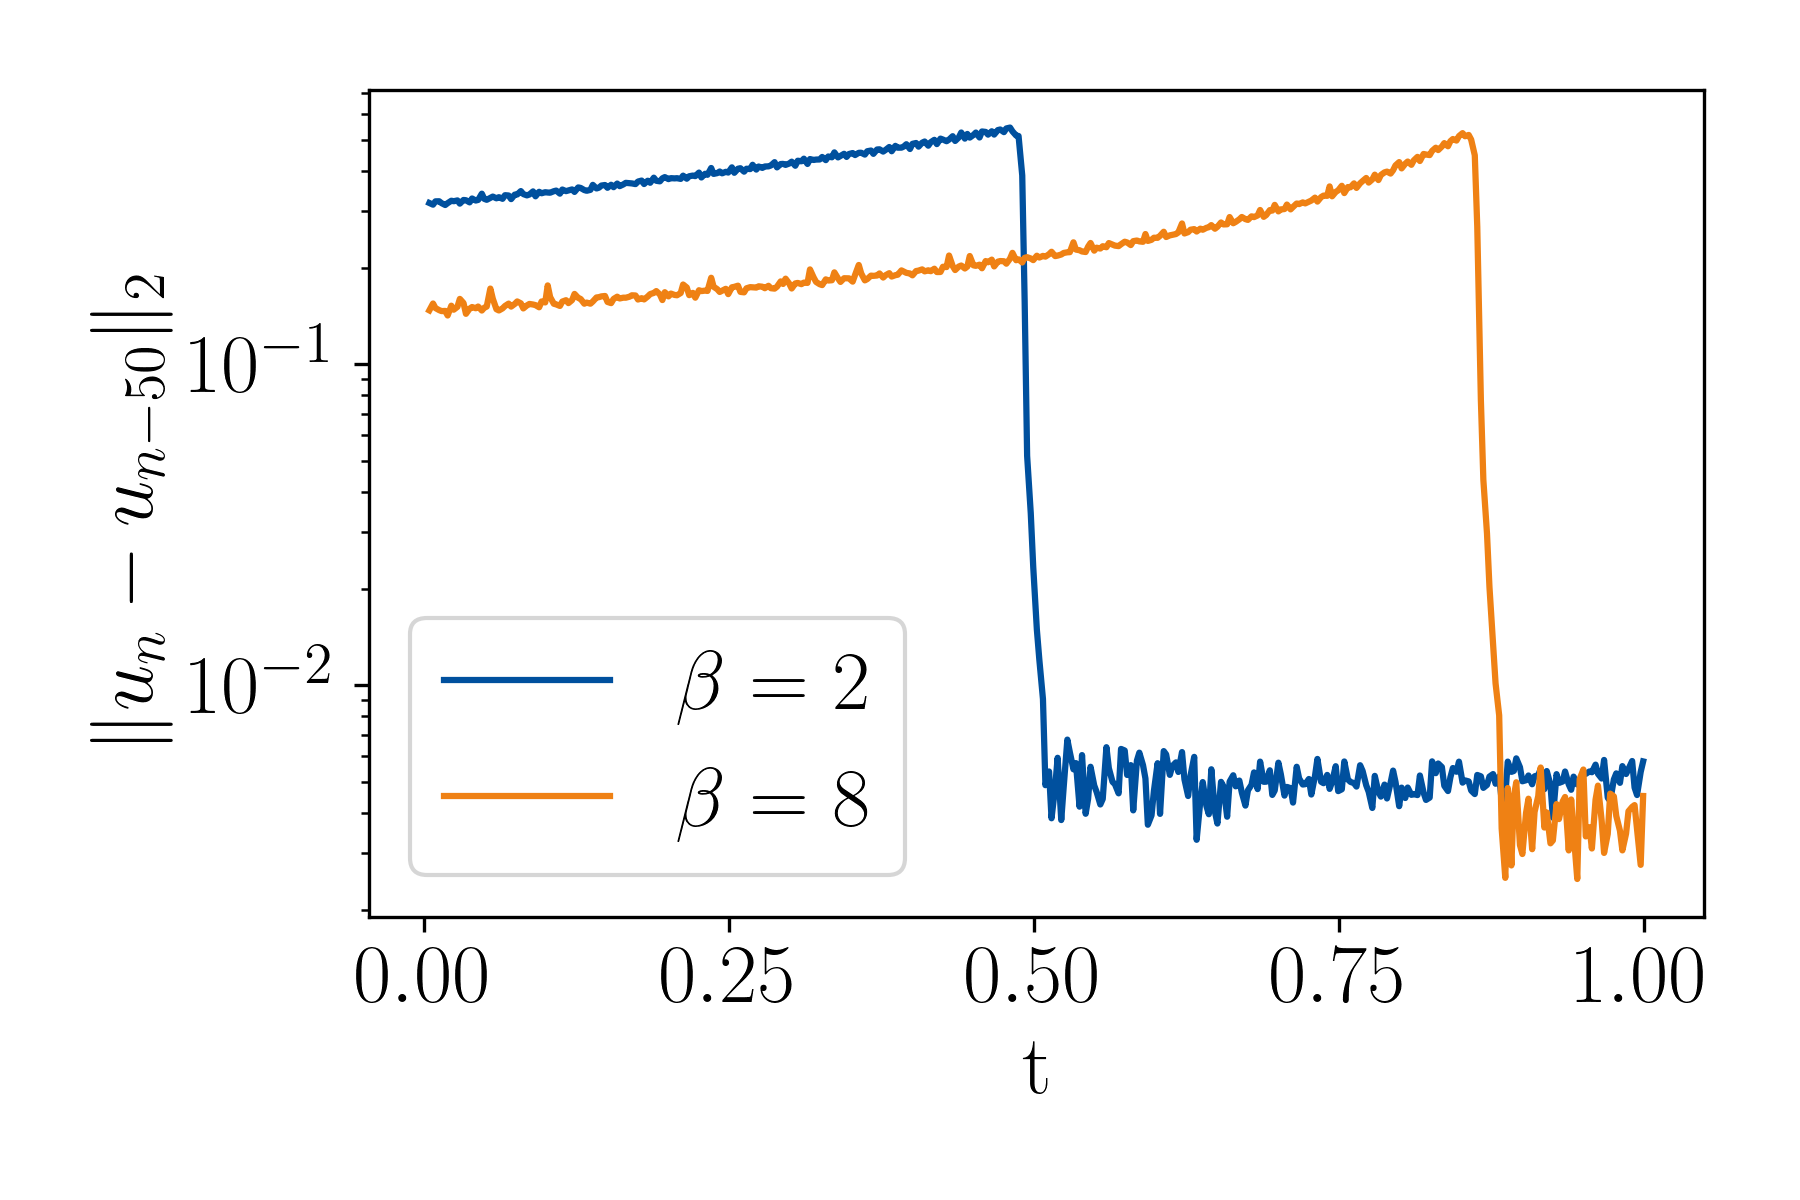
\includegraphics[width=\linewidth]{figures/Results/Circle/model3/b2_b8_res.png}
    \end{subfigure}
    \caption[Model 3 - Circular example, $\beta$ parameter]{Model 3: $h=0.01$, $10$ level curves, $\alpha=0.9$, $dt=1/2 h^2$, $r_0=0.9$, $200$ points. Reinitialized every $50$ iteration}
    \label{fig:model3-circle-betas}
\end{figure}
Furthermore, we observe from the residual plot in \figref{fig:model3-circle-betas}, that $\beta$ does not have much effect on the final curve, but higher $\beta$ makes everything go slower. Since $\beta=2$ moves faster up to the point set and have more or less the same amplitude of oscillations, this seems like a better choice. We suspect that the reason why the final curve behaves so similarly is that the point set is so dense that the distance approaches zero for both values of $\beta$, and then $f_3\to 1$ for both cases. The scaling only influences the movement when the distance is bigger, hence on the way in. 

\newpage
\section{Test Case 2: Three Equidistant Points}
We have now seen how the numerical models performed compared to the theoretical analysis and also how the solutions varied with the parameters. The circle example did not provide so interesting contour plots because of the symmetry. The next test case will provide some more freedom for the curve because the points are further apart. We will also see how the curvature will vary when the distance function changes over the curve.

Again, we open with model 1. We see some interesting behavior in the contour plot in \figref{fig:m1-three-a96}. Now we for the first time need to be attentive when we follow the curve over time. We see that it begins as the initial circle with $r_0=0.9$ and at first it moves inwards and reaches the point set looking similar to a triangle with edges in the sample points. Even though the curve has reached the point set, it does not stop changing shape then. As we can see from the velocity function in \eqref{eq:model1-pde}, when the distance is zero, the curvature must also be zero to stop the motion. Thus, the curve still moves inwards close to the points, which changes the sign function. Thus all parts of the curve where $\alpha d > (1-\alpha)\kappa$ starts moving outwards again. This again reduces the curvature, and the curve close to the points approaches the point set again. 

\begin{figure}
    \centering
    \begin{subfigure}[h]{0.49\textwidth}
        \centering
        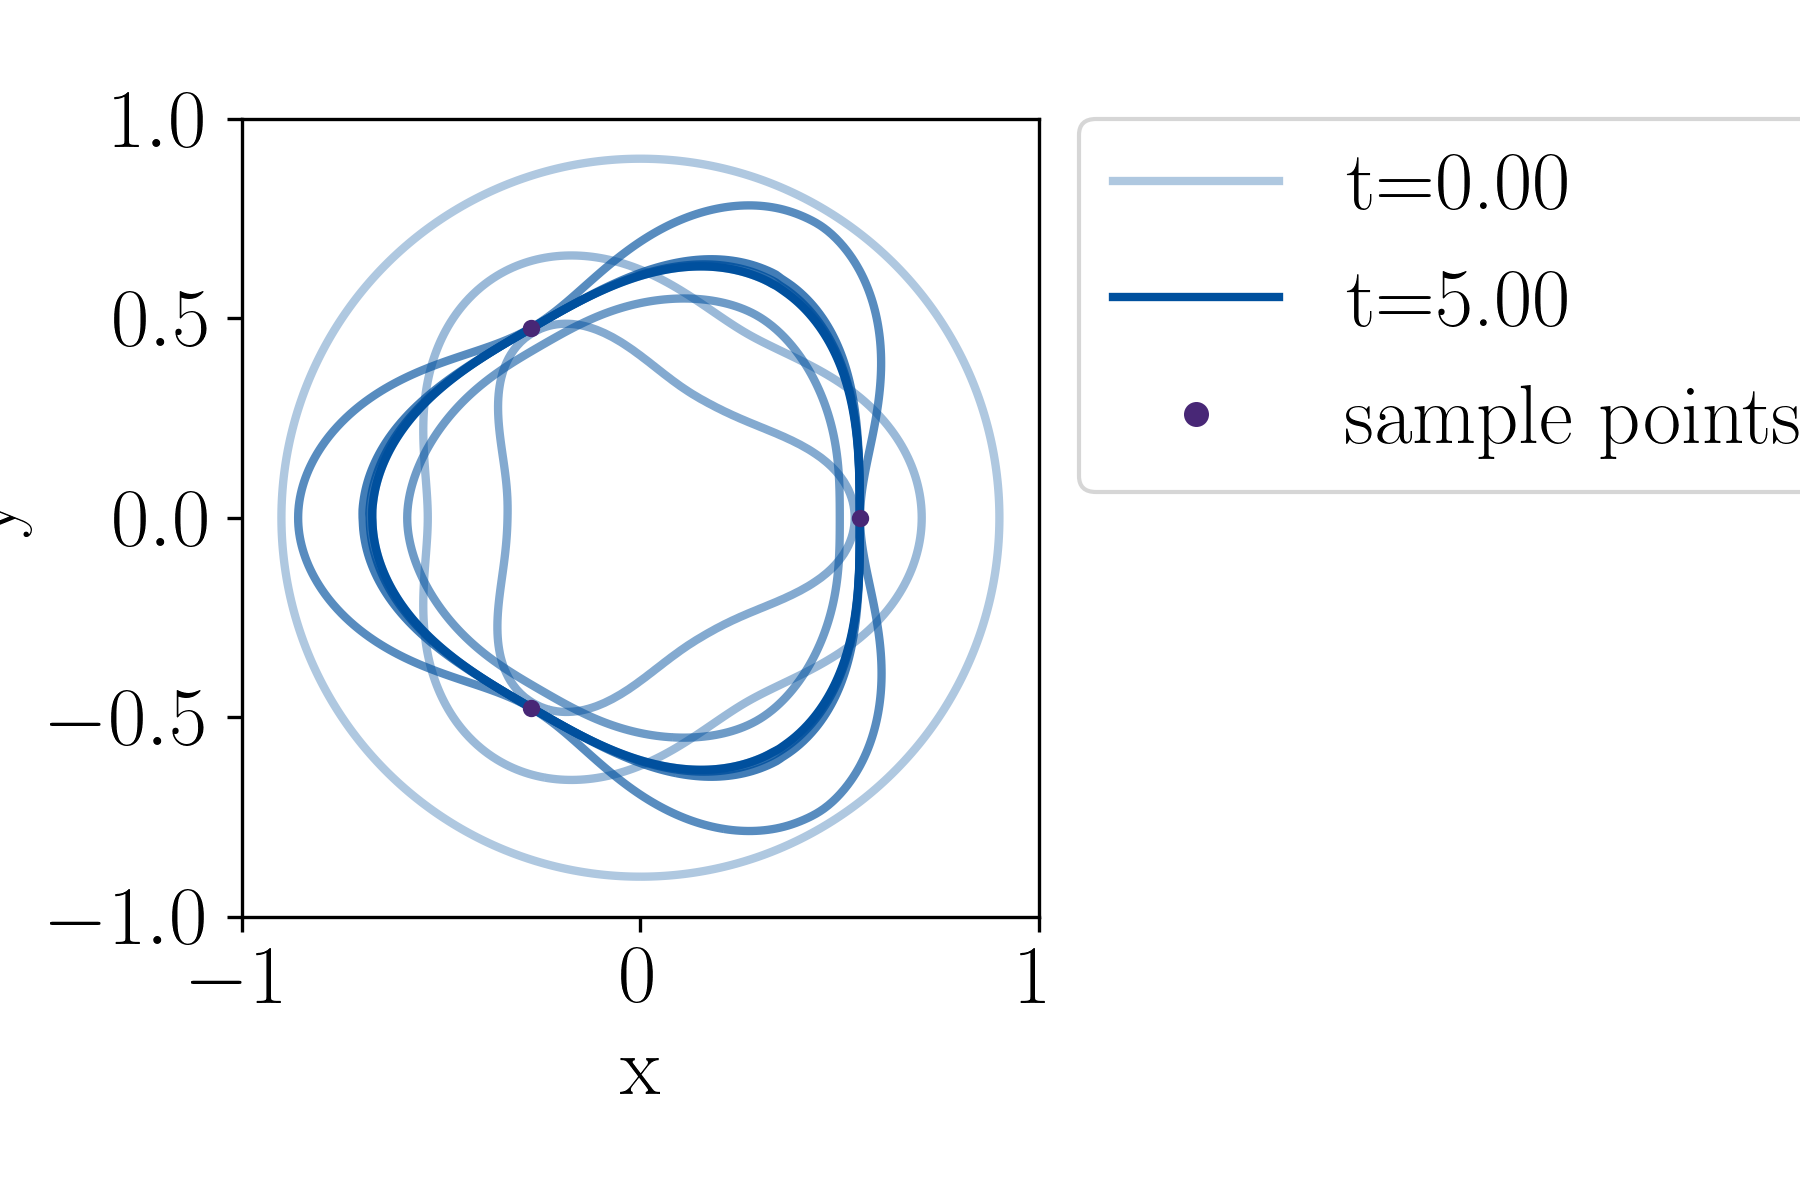
\includegraphics[width=\linewidth]{figures/Results/Three-points/model1/threepoints-a96.png}
        \caption{$\alpha=0.96$}
        \label{fig:m1-three-a96}
    \end{subfigure}%
    \begin{subfigure}[h]{0.49\textwidth}
        \centering
        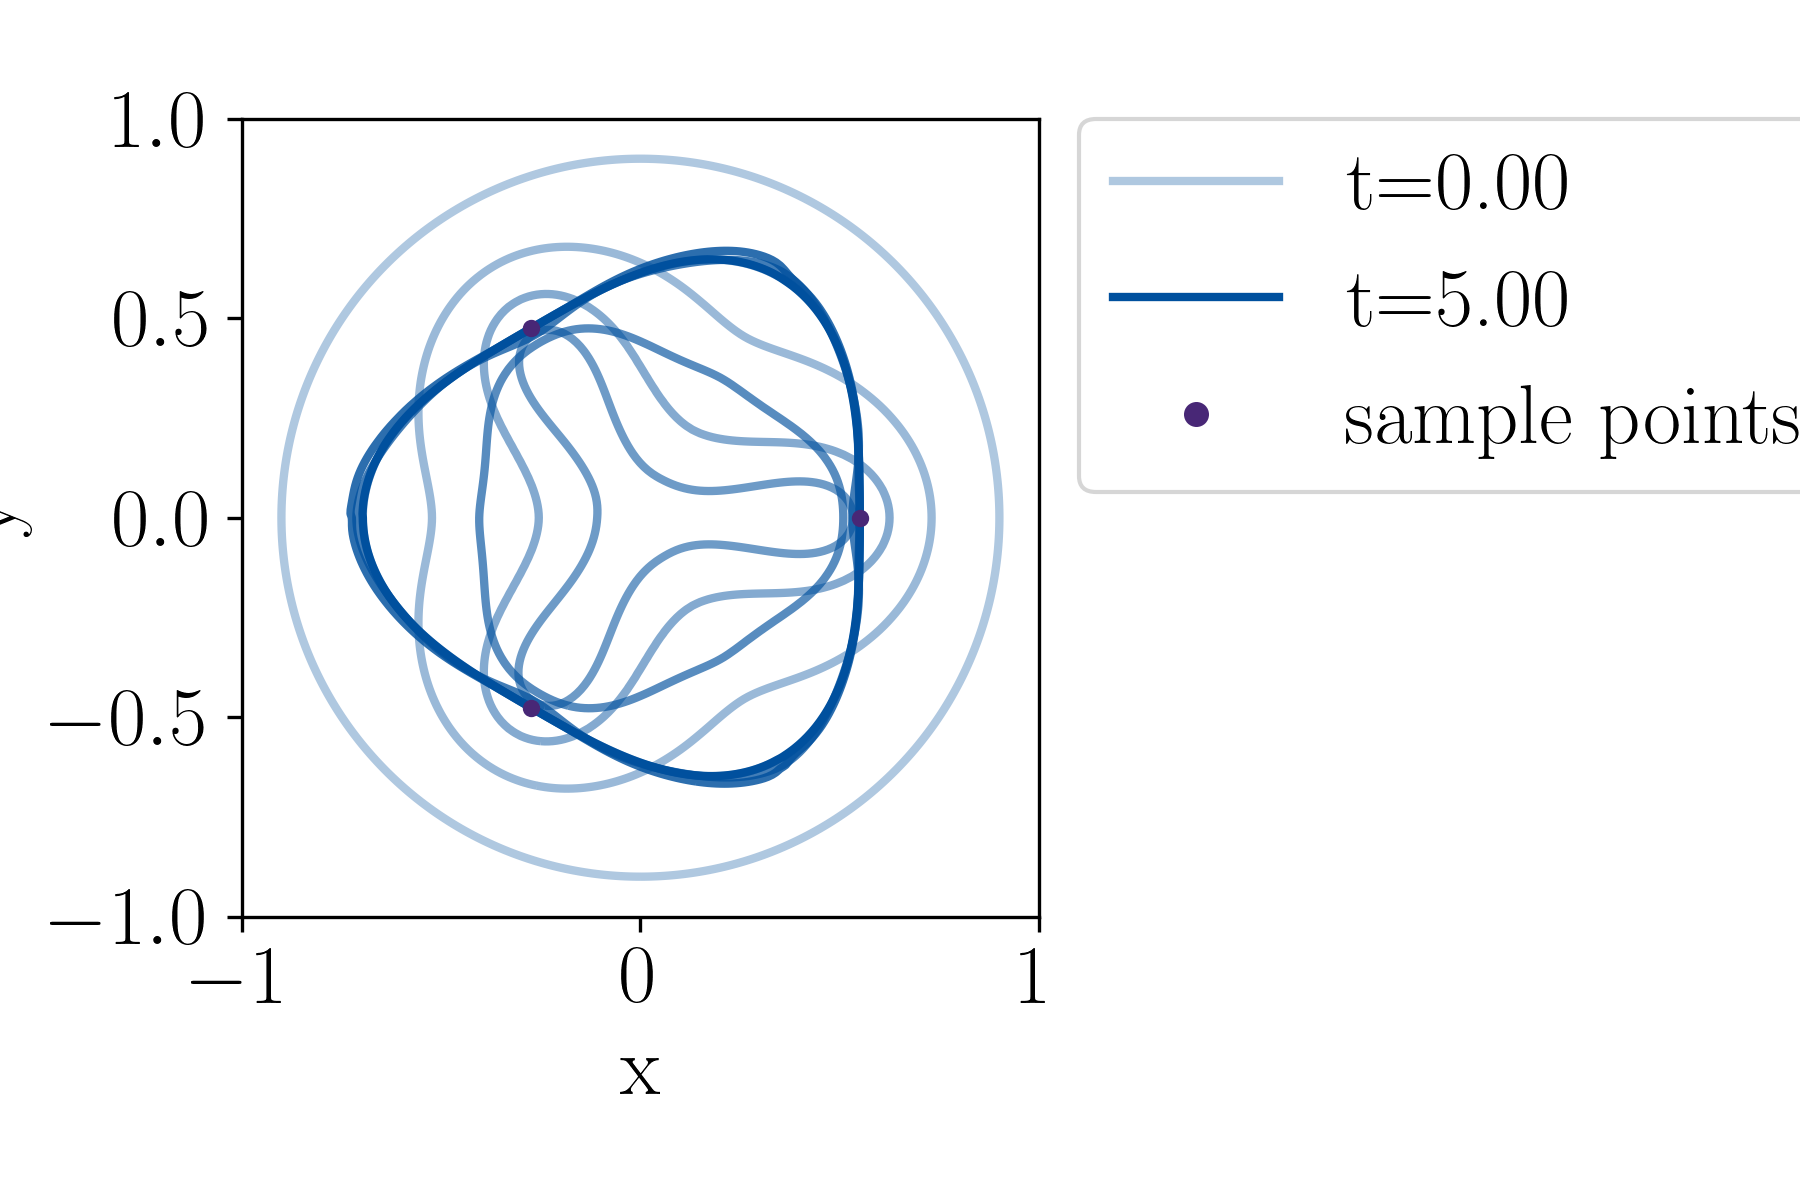
\includegraphics[width=\linewidth]{figures/Results/Three-points/model1/threepoints-a99.png}
        \caption{$\alpha=0.99$}
        \label{fig:m1-three-a99}
    \end{subfigure}
\caption[Model 1 - Triangle, $\alpha=0.96$]{Model 1: $h=0.01$, $9$ level curves, $r_0=0.9$, reinitialize every $50$ steps}
\label{fig:m1-three-points}
\end{figure}


It is interesting that the curve has such different shapes during the evolution, and after the curve hits the points for the first time, any of the plotted contours would be nice curve reconstructions provided the three sampled points. Finally, we must note that the curve do not slow down nicely as we saw in \figref{fig:model1-sigma-dist-full}. We see from the contours that the last $4$ curves are almost inseparable, but the contour plot together with the residual plot says that the curve do not reach a totally stationary solution. We actually observe oscillations for model 1 as well.

When we increase $\alpha$, the curve sections that are far from the sample points will move faster than before. This is also what we see in \figref{fig:m1-three-a99}, where the sections between the curve points move so much faster than the sections close to the point set that they are almost making contact before the sign changes and they move outward again. Here we can see that the model is sensitive for the choice of $\alpha$, and if chosen too high, the curve sections will merge in the middle and split into islands which will disappear into nothing.

Also note that increasing $\alpha$ must lead to a stationary curve having greater curvature further from the points, and this is also what we see in \figref{fig:m1-three-a99} as the last curves are somewhat sharper than in \figref{fig:m1-three-a96}. Although, we must say that this choice of $\alpha$ does not either obtain a stationary curve as it too oscillates after about $t\sim 4$. We also see from the residual plot in \figref{fig:m1-three-res}, that both choices of $\alpha$ yields very similar oscillations, so the difference is mostly seen in the shape of the final contour. The time it takes for the curve with $\alpha=0.99$ to stop is somewhat longer because it both moves closer to the middle and ends up with a curve that is a bit bigger than for $\alpha=0.96$.


\begin{figure}
    \centering
    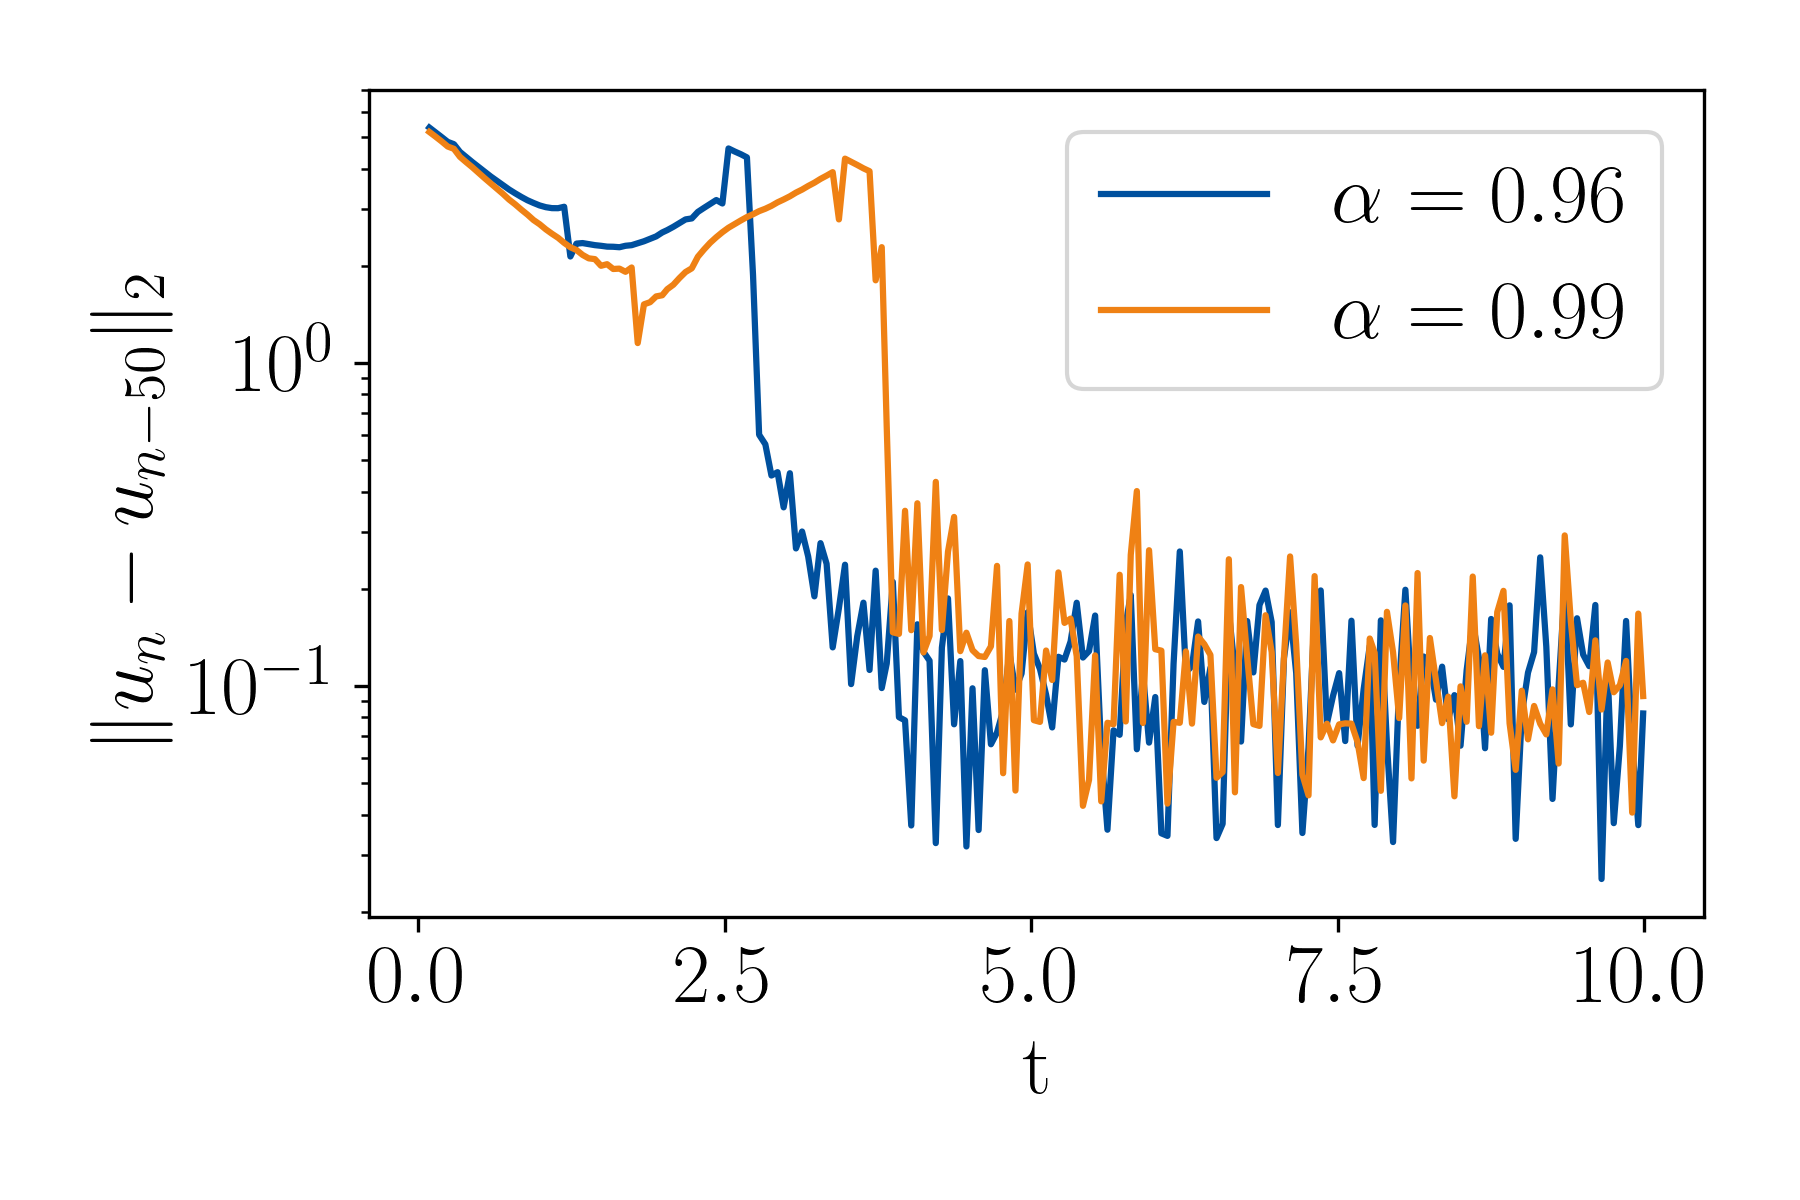
\includegraphics[width=.6\linewidth]{figures/Results/Three-points/model1/a96_a99_res.png}
    \caption[Model 1 - Triangle, Residuals]{Model 1: $h=0.01$, $9$ level curves, $r_0=0.9$, reinitialize every $50$ steps}
    \label{fig:m1-three-res}
\end{figure}

When we look at the final curve obtained for model 2 in \figref{fig:m2-threepoints-04}, we see a totally different picture than for model 1. The curves moves slower in the beginning, which we saw from the first test case also and the parts of the curve furthest from the point set moves slowest. However, in contrast to model 1, the curve obtains its final shape on the way in. The final shape is also a completely different approach to reconstructing a curve and yields highest curvature at the point set. A disappointing fact we can see from the residual plot in \figref{fig:m2-threepoints-04} is that we still have oscillations.

\begin{figure}
\begin{center}
\resizebox{.99\textwidth}{!}{%
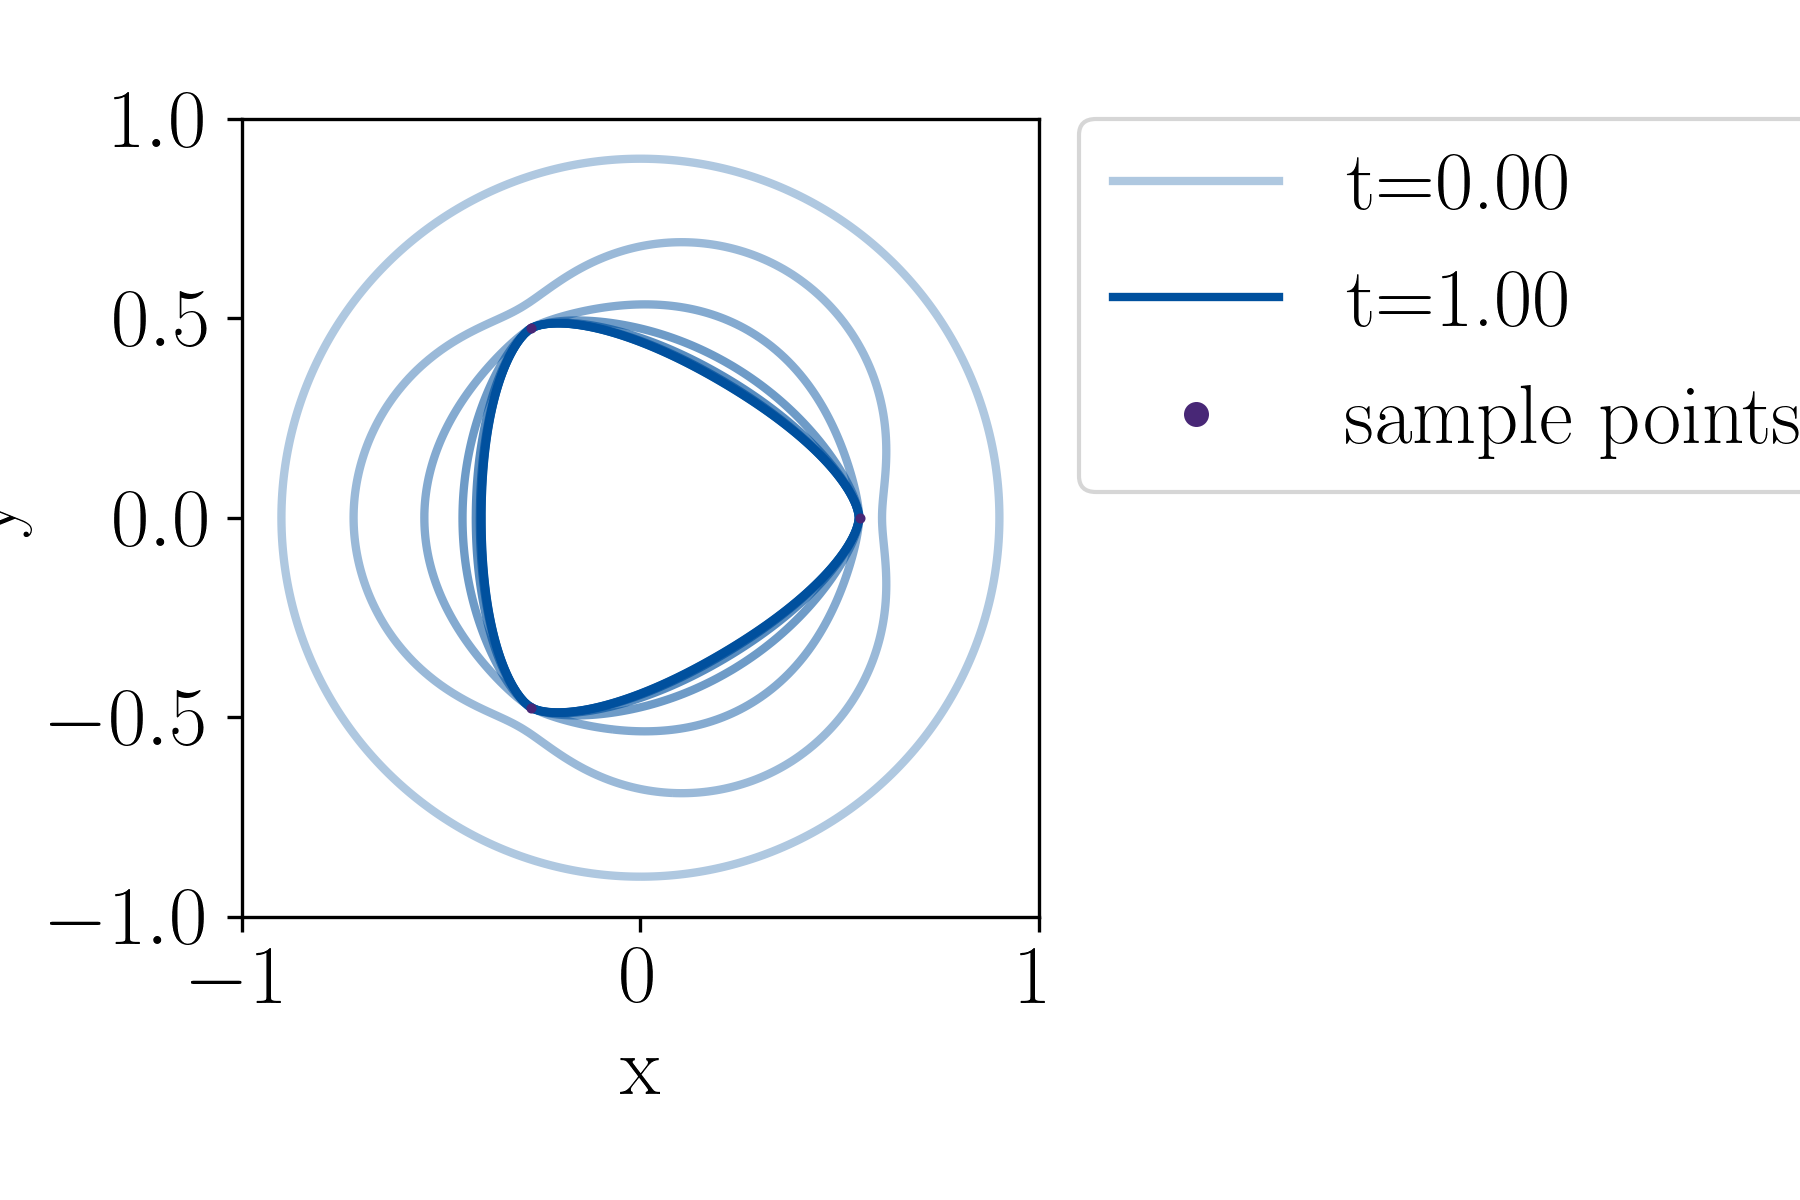
\includegraphics[height=3.5cm]{figures/Results/Three-points/model2/threepoints-a04.png}%
\,
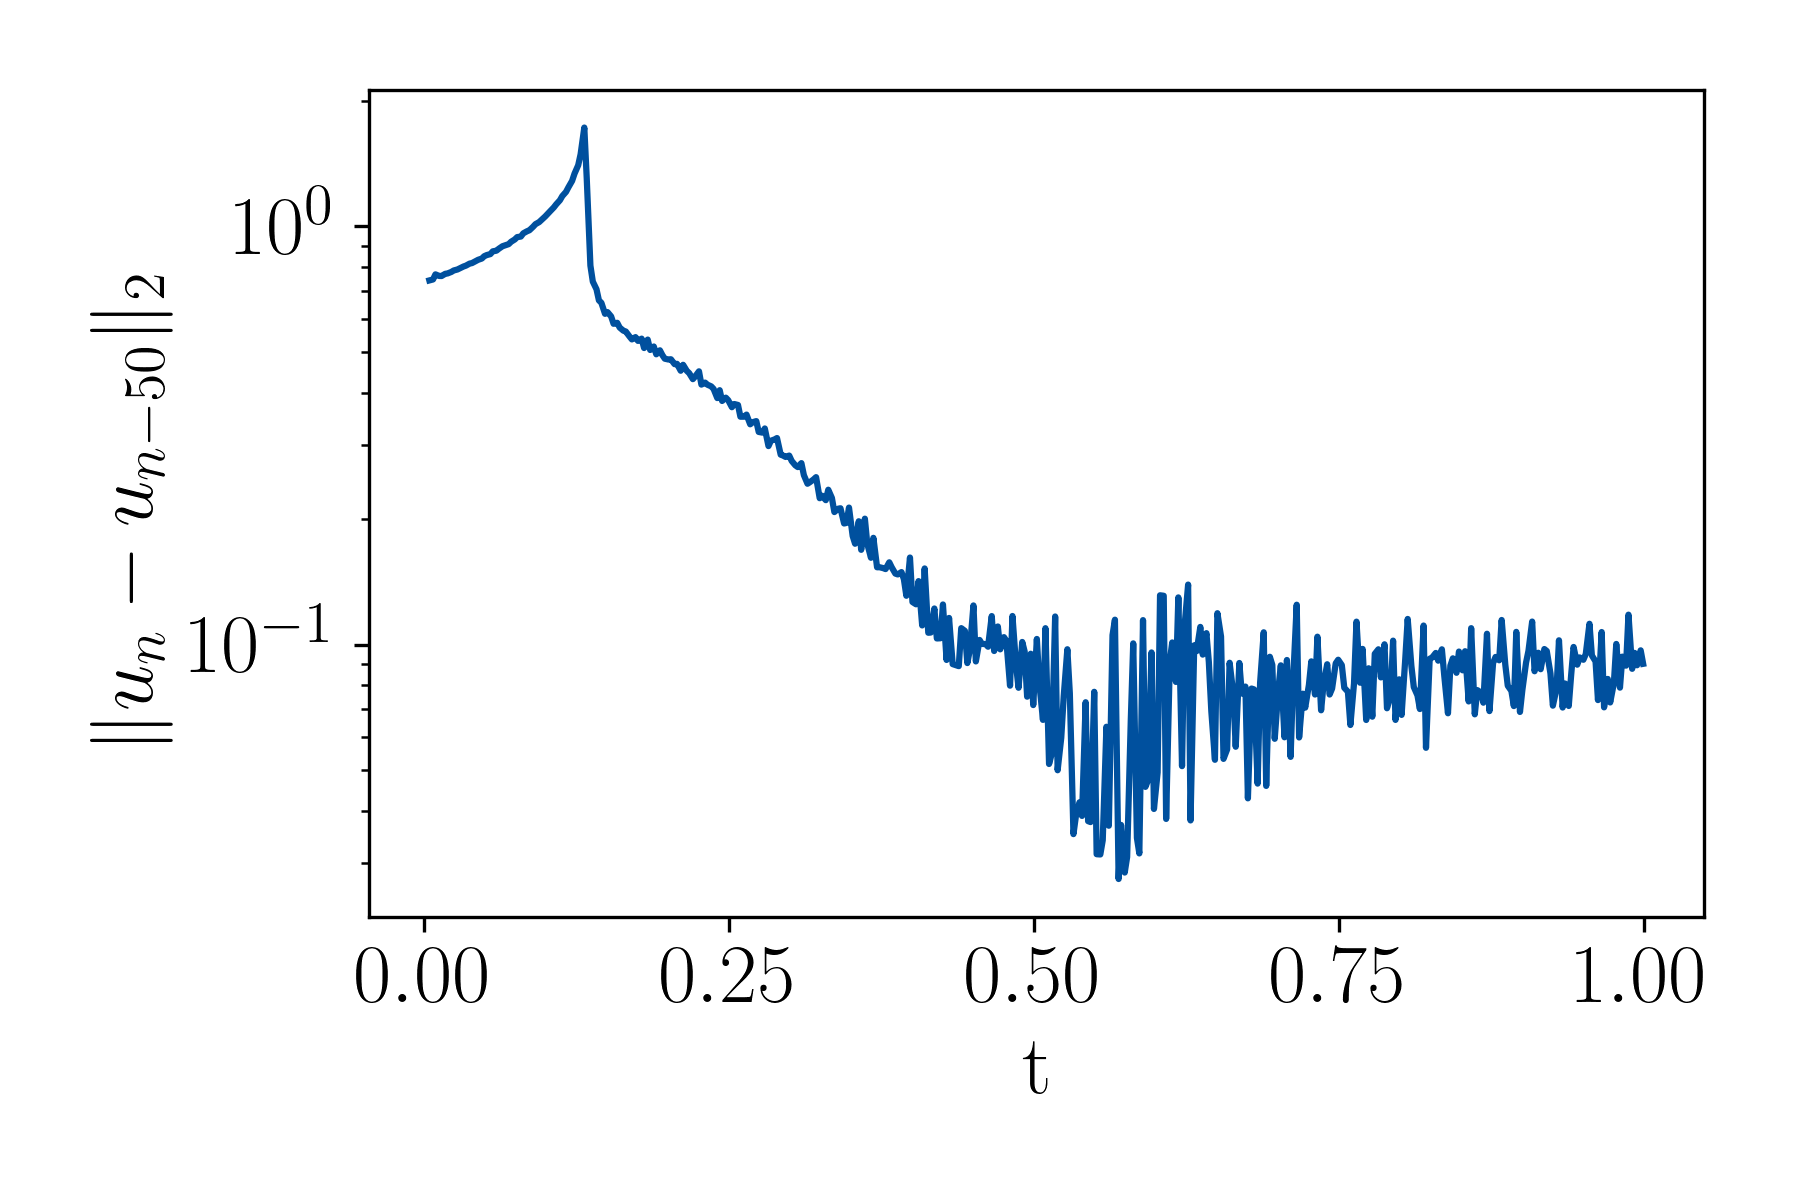
\includegraphics[height=3.5cm]{figures/Results/Three-points/model2/three-a4-logy.png}%
}
\end{center}
\vspace{-2.5em}
\caption[Model 2 - Triangle, $\alpha=0.4$]{Model 2: $h=0.01$, $9$ level curves, $\alpha=0.4$, $\delta=10^{-2}$, $r_0=0.9$, reinitialize every $50$ steps}
\label{fig:m2-threepoints-04}
\end{figure}

In order to observe how sensitive also this model is concerning the choice of $\alpha$, we take a quick look at what happens when $\alpha=0.2$ in stead. The simulation is run until $t=0.5$ and displayed in \figref{fig:m2-threepoints-02}. We see that the last curve is inside the point set and from the residual plot, we see that the movement is speeding up. The curve is on its way inwards and the curvature driven speed is dominating and driving it into disappearing in the middle, but we have stopped the simulation before it disappears. Here we can thus see what happens if $\alpha$ is too small and the curvature dominates the motion. 

This is also a reason why a stopping criterion based on the velocity may be a bad idea. We see in the residual plot that the curve is slowing down and it may seem like it is stabilizing, but suddenly it starts moving inwards and the solution slips. Thus what seemed like a final curve was not close at all.

\begin{figure}
\begin{center}
\resizebox{.99\textwidth}{!}{%
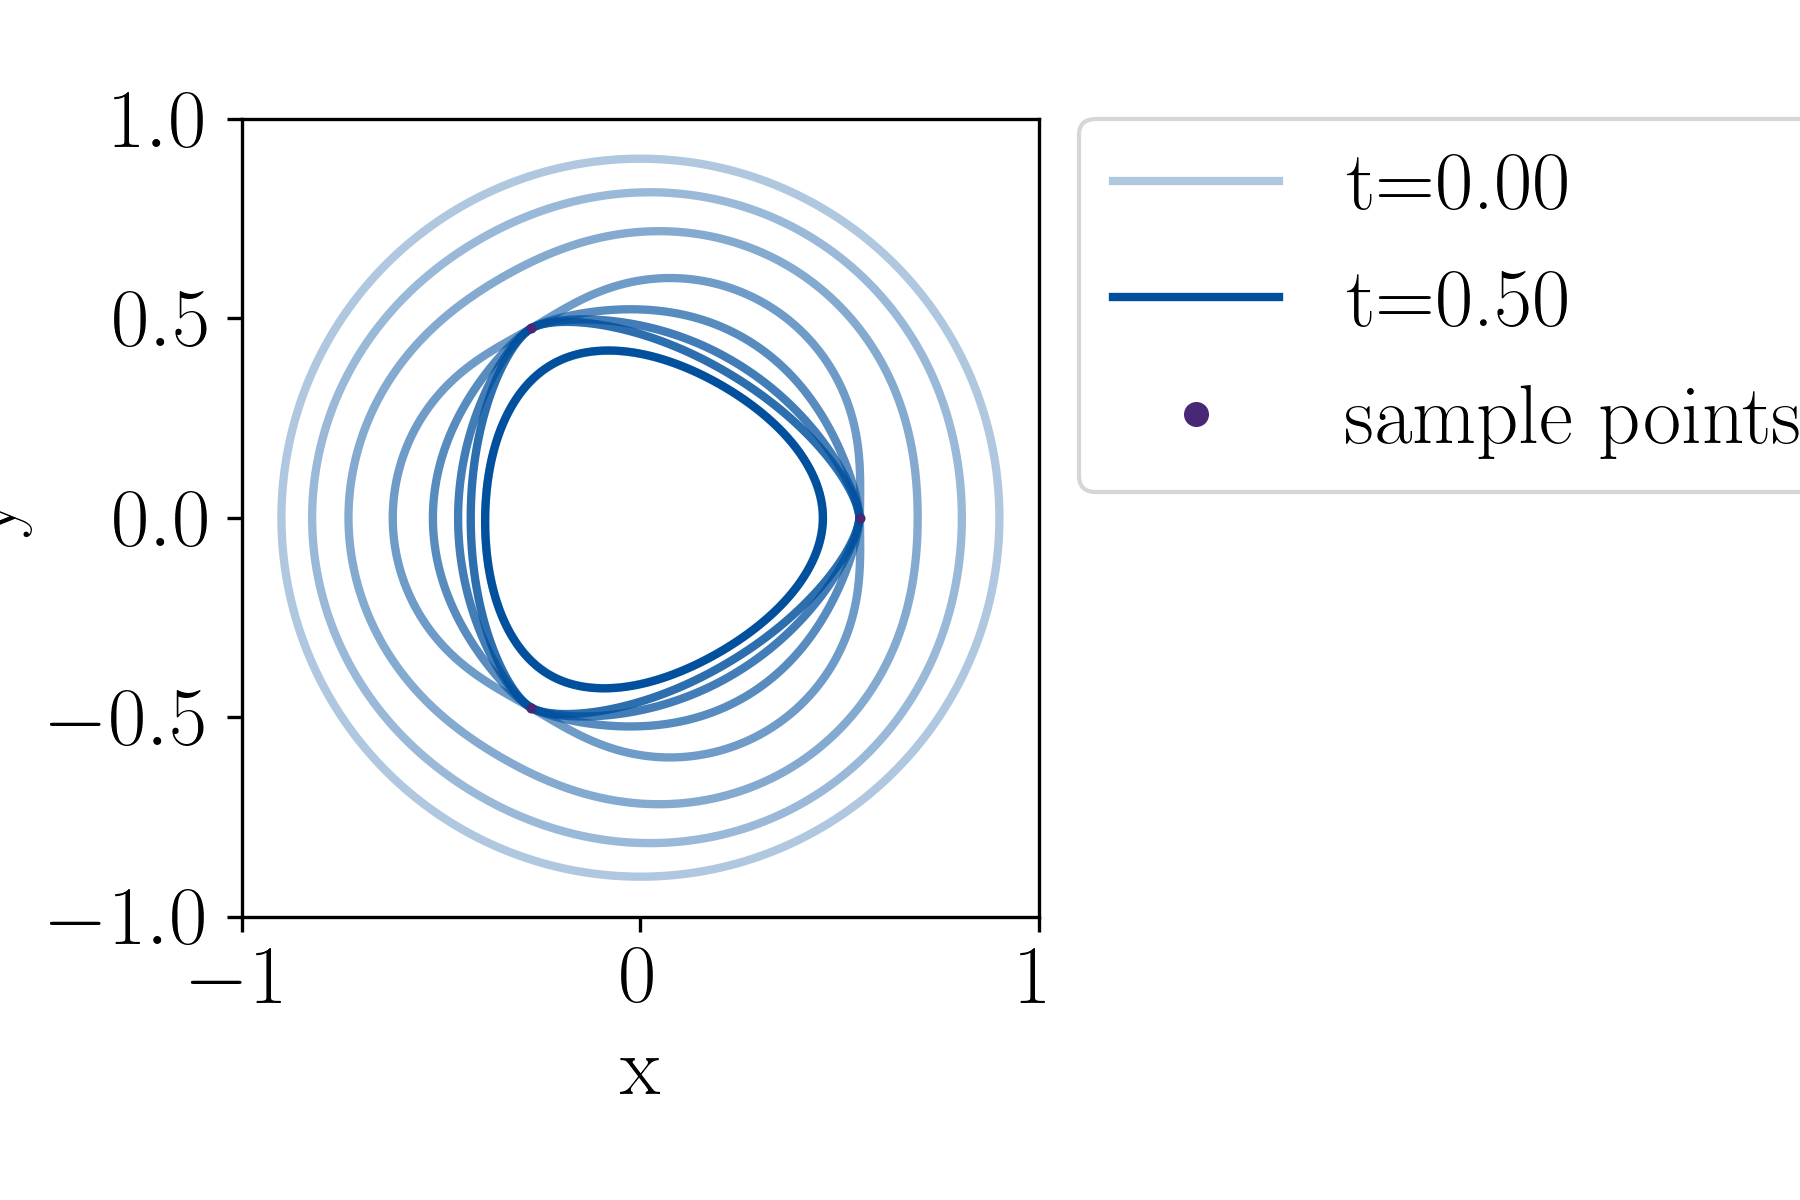
\includegraphics[height=3.5cm]{figures/Results/Three-points/model2/threepoints-a02.png}%
\,
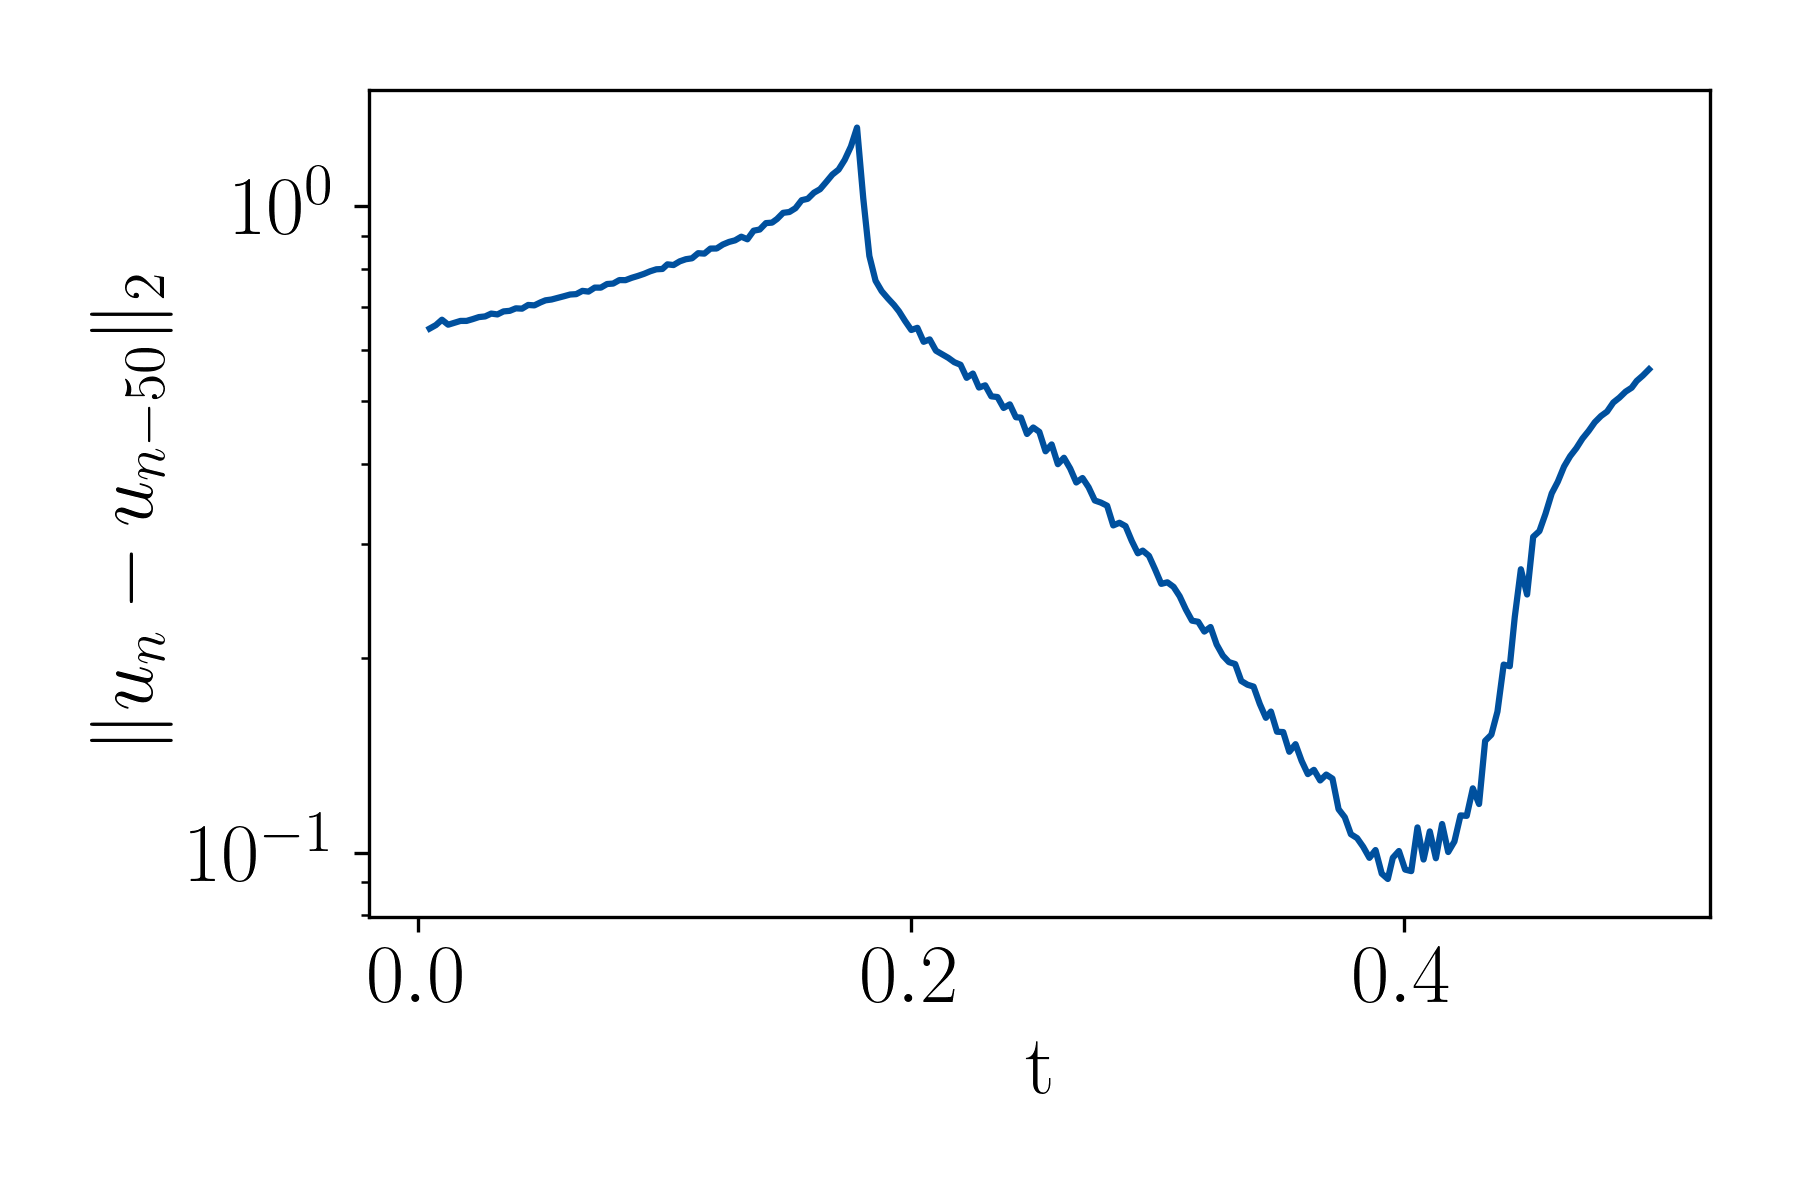
\includegraphics[height=3.5cm]{figures/Results/Three-points/model2/three-a02-logy.png}%
}
\end{center}
\vspace{-2.5em}
\caption[Model 2 - Triangle, $\alpha=0.2$]{Model 2: $h=0.01$, $9$ level curves, $\alpha=0.2$, $\delta=10^{-2}$, $r_0=0.9$, reinitialize every $50$ steps}
\label{fig:m2-threepoints-02}
\end{figure}


Moving over to model 3, we see in \figref{fig:m3-three-b2} for $\alpha=0.9$ and $\beta=2$, that similarly to model 2, the curve is sharpest near the points as expected. The curve is though much rounder than what we saw in \figref{fig:m2-threepoints-02}. To make the edges sharper, one could scale the distance by increasing $\beta$ which is done in \figref{fig:m3-three-b8}.

\begin{figure}
    \centering
    \begin{subfigure}[h]{0.49\textwidth}
        \centering
        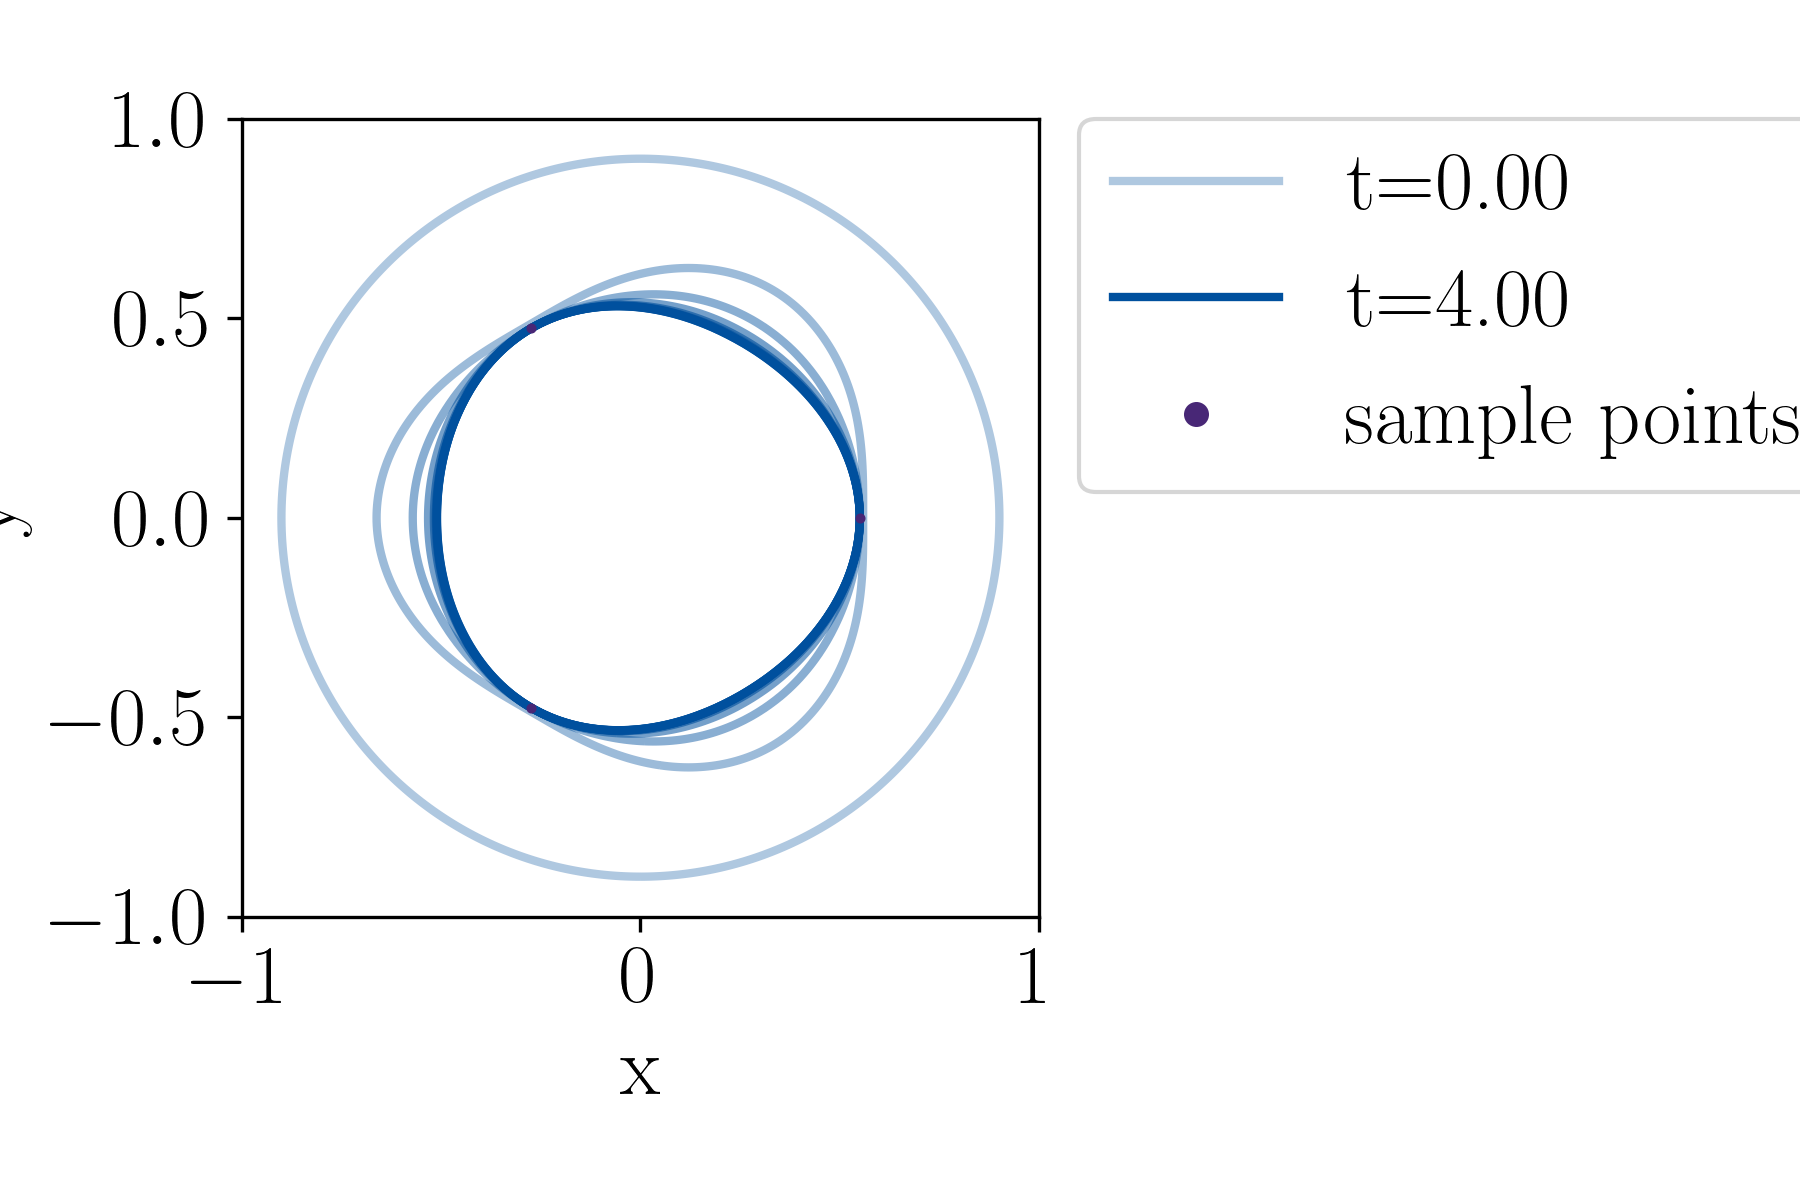
\includegraphics[width=\linewidth]{figures/Results/Three-points/model3/three-a9-b2-t4-conts.png}
        \caption{$\beta=2$}
        \label{fig:m3-three-b2}
    \end{subfigure}%
    \begin{subfigure}[h]{0.49\textwidth}
        \centering
        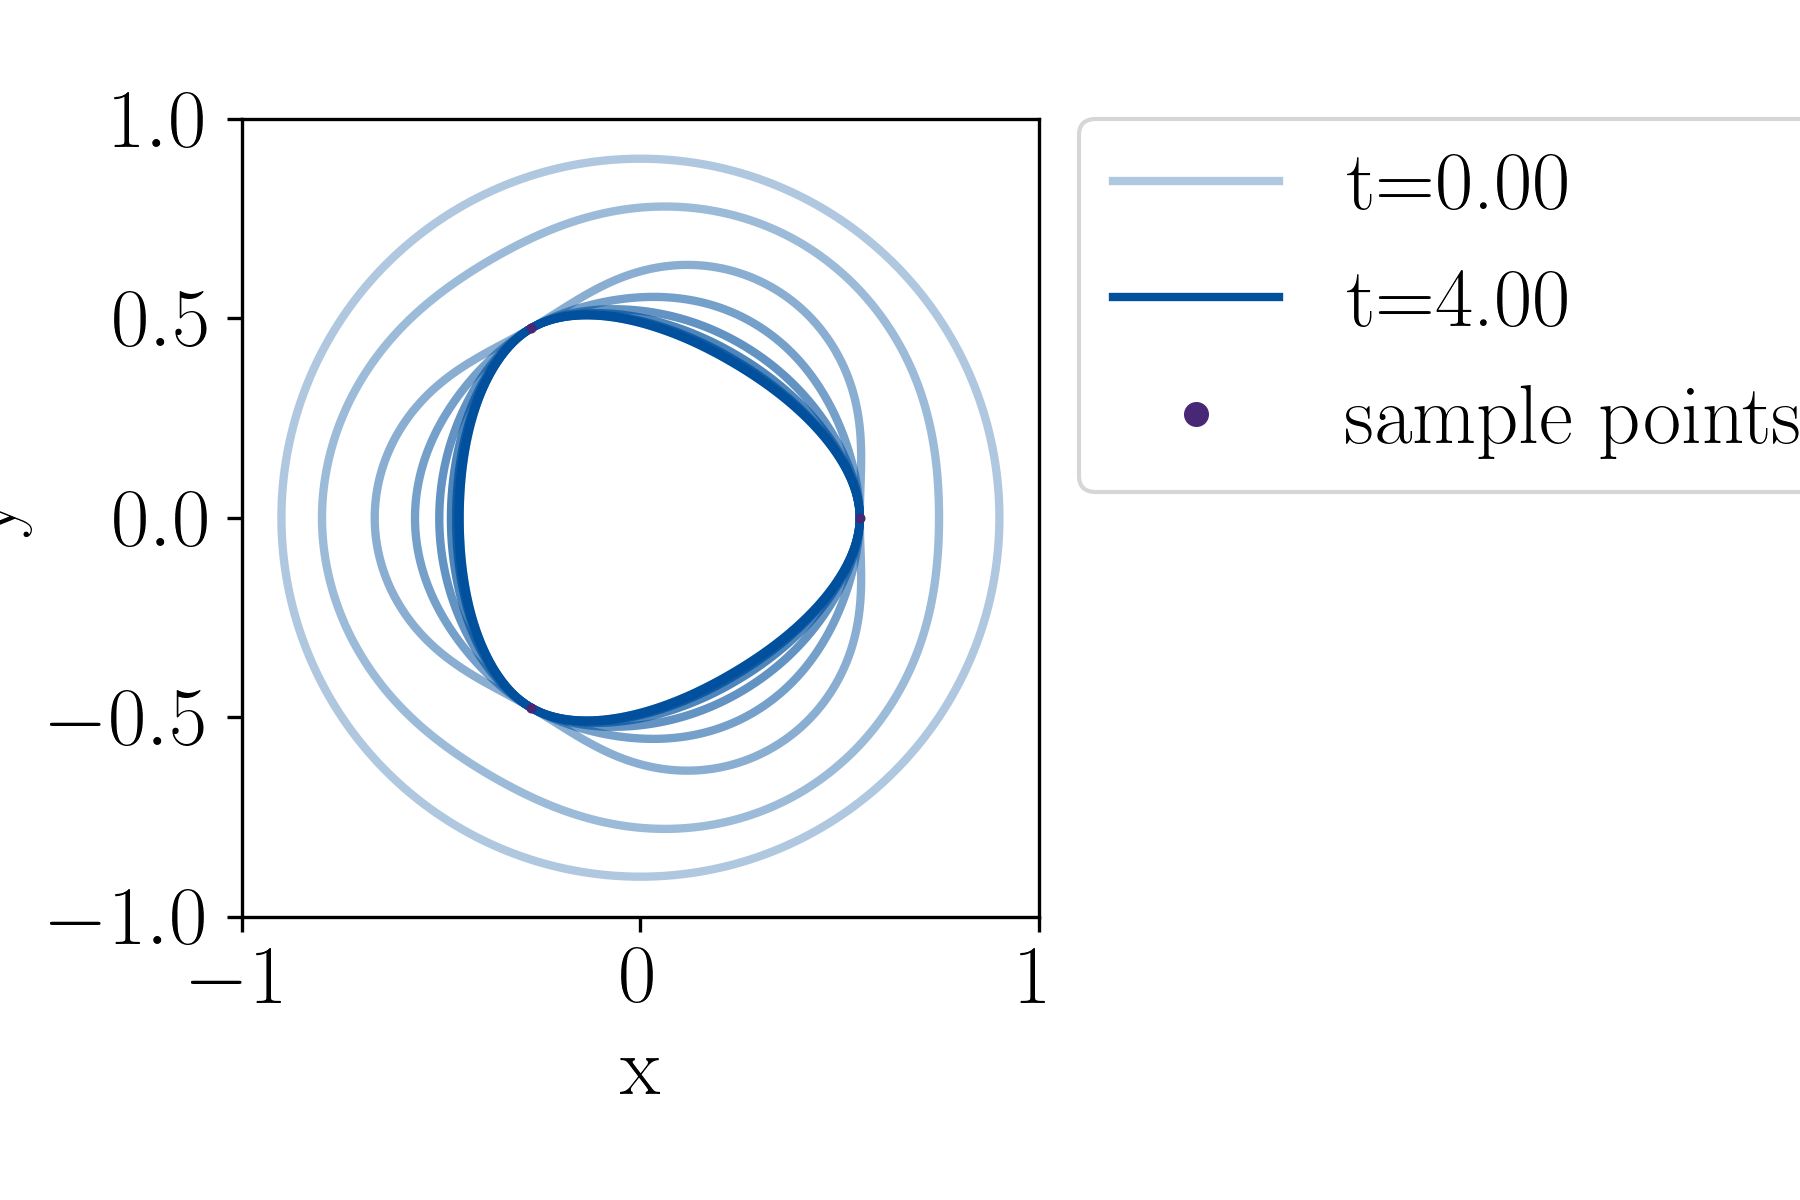
\includegraphics[width=\linewidth]{figures/Results/Three-points/model3/three-a9-b8-t4-conts.png}
        \caption{$\beta=8$}
        \label{fig:m3-three-b8}
    \end{subfigure}
\caption[Model 3 - Triangle, $\beta=2$ and $\beta=8$]{Model 3: $h=0.01$, $10$ level curves, $r_0=0.9$, $\alpha=0.9$, reinitialize every $50$ steps}
\label{fig:m3-three-points-conts}
\end{figure}

\begin{figure}
    \centering
    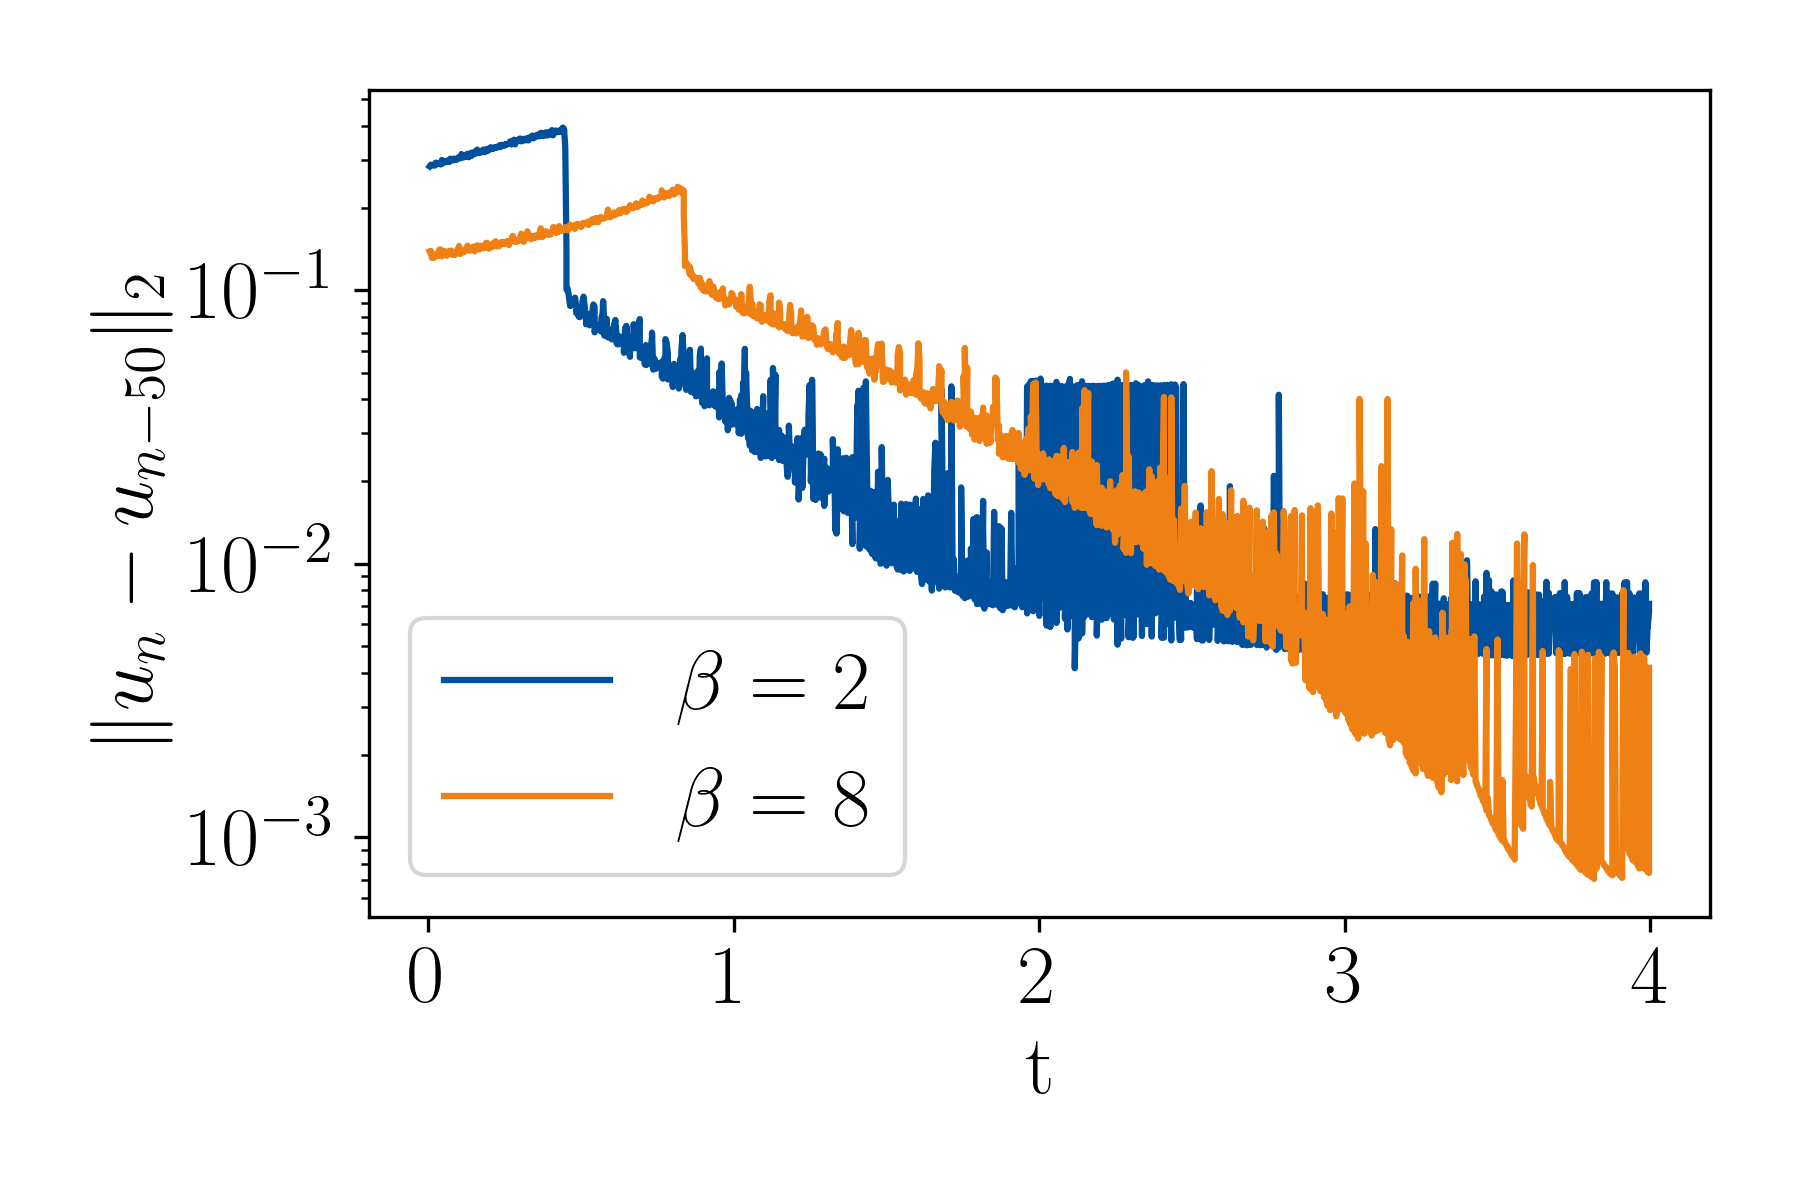
\includegraphics[width=.6\linewidth]{figures/Results/Three-points/model3/b2_b8_res-t4.png}
    \caption[Model 3 - Triangle, Residuals]{Model 1: $h=0.01$, $9$ level curves, $r_0=0.9$, reinitialize every $50$ steps}
    \label{fig:m3-three-res}
\end{figure}


Even though the final curves obtain a similar shape as for model 2, we see that the residual plot for both values of $\beta$ displayed in \figref{fig:m3-three-res} are very different. We see a curve gradually slowing down and obtaining a considerably lower speed than in \figref{fig:m2-threepoints-04} and \figref{fig:m2-threepoints-02}. 

\clearpage
\section{Test Case 3: Dense and Irregular Data}
In this test case, it is much easier to conclude on whether or not the curves provide a good solution. We begin with the first model with $\alpha=0.99$. The contours in \figref{fig:m1-manypoints-a99} shows that the curves quickly obtains a shape similar to the point set, and that the final curve looks approximates the point better than the early times. The final curve fulfills the goal of approximate the point set while having small curvature, although it is slightly more on the inside than it is outside the point set. Furthermore, we see that in the region up to the right where the points are almost on a straight line, the final curve would have filtered the data nicely if the deviations were noise. 

\begin{figure}
\begin{center}
\resizebox{.99\textwidth}{!}{%
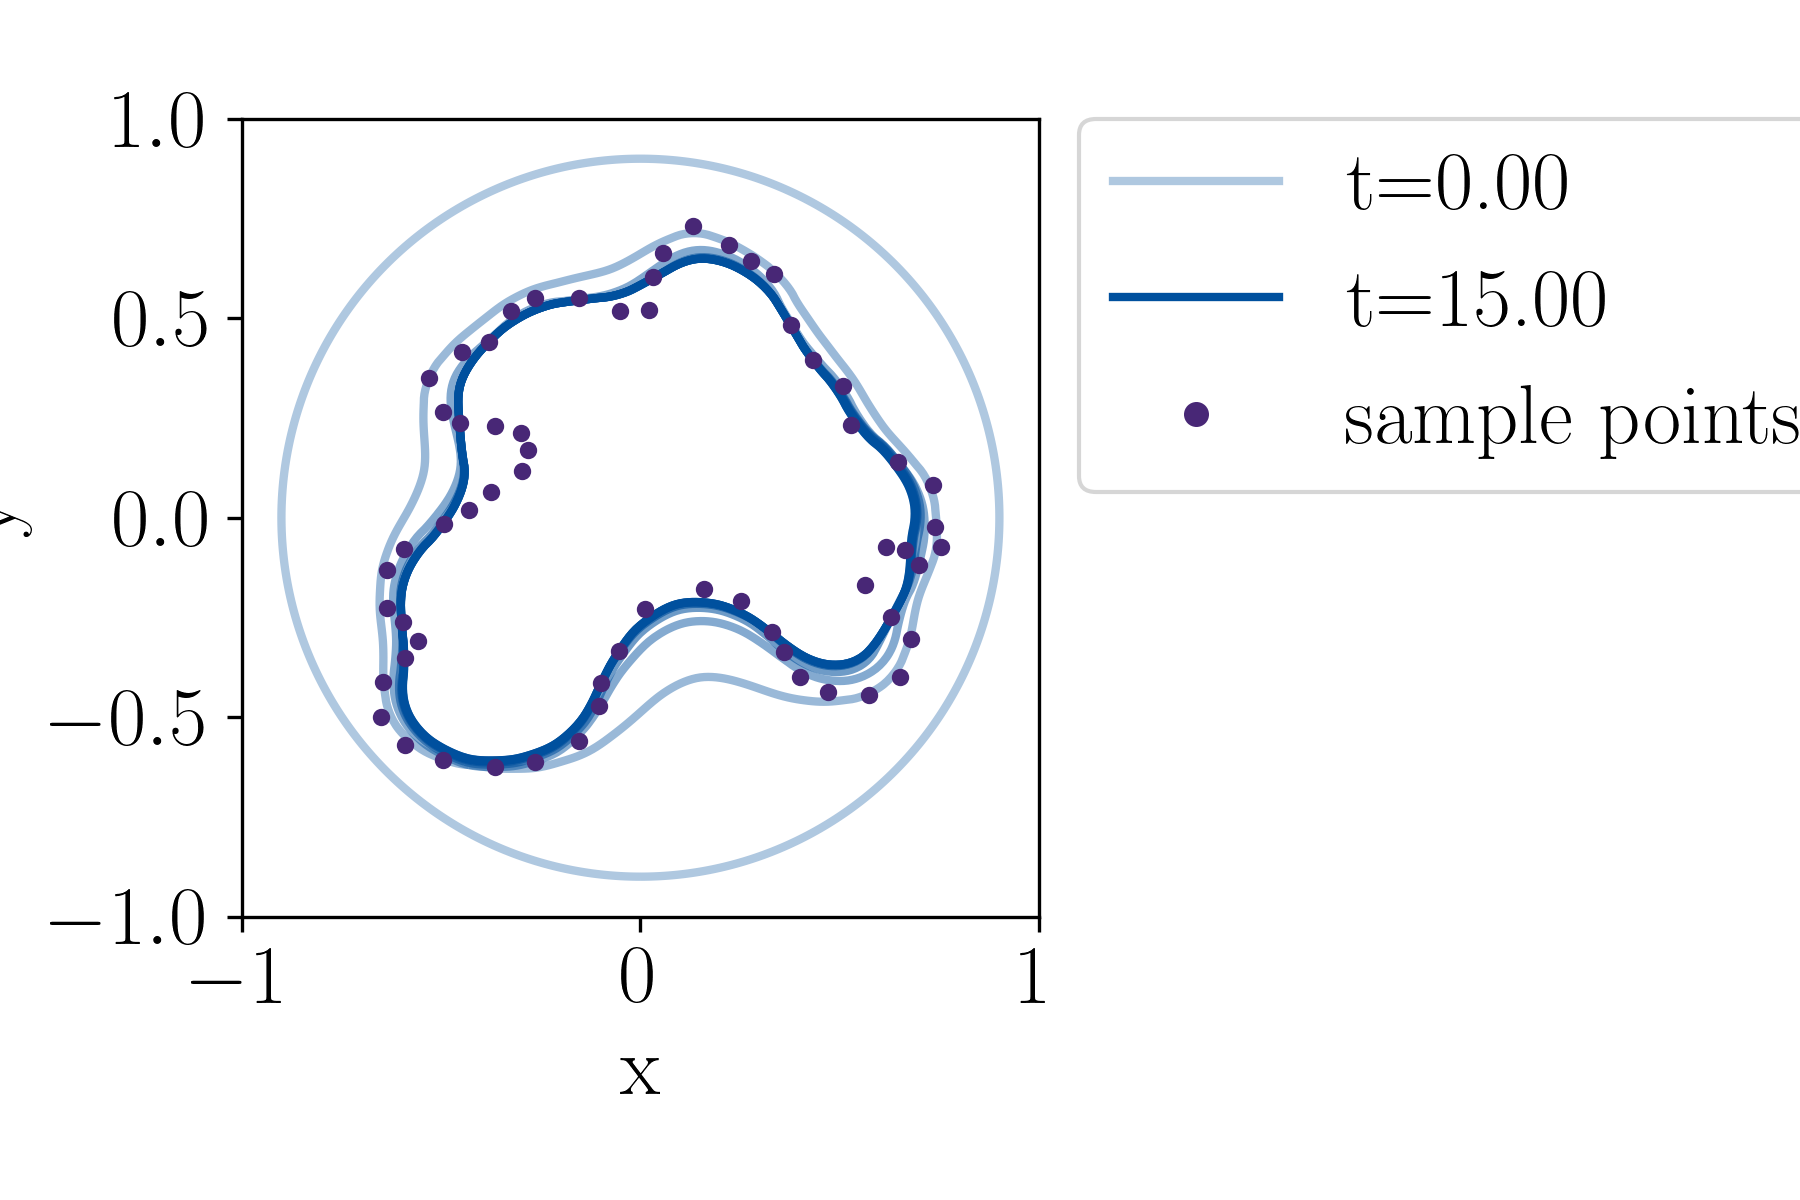
\includegraphics[height=3.5cm]{figures/Results/Many-points/model1/manypoints-a99.png}%
\,
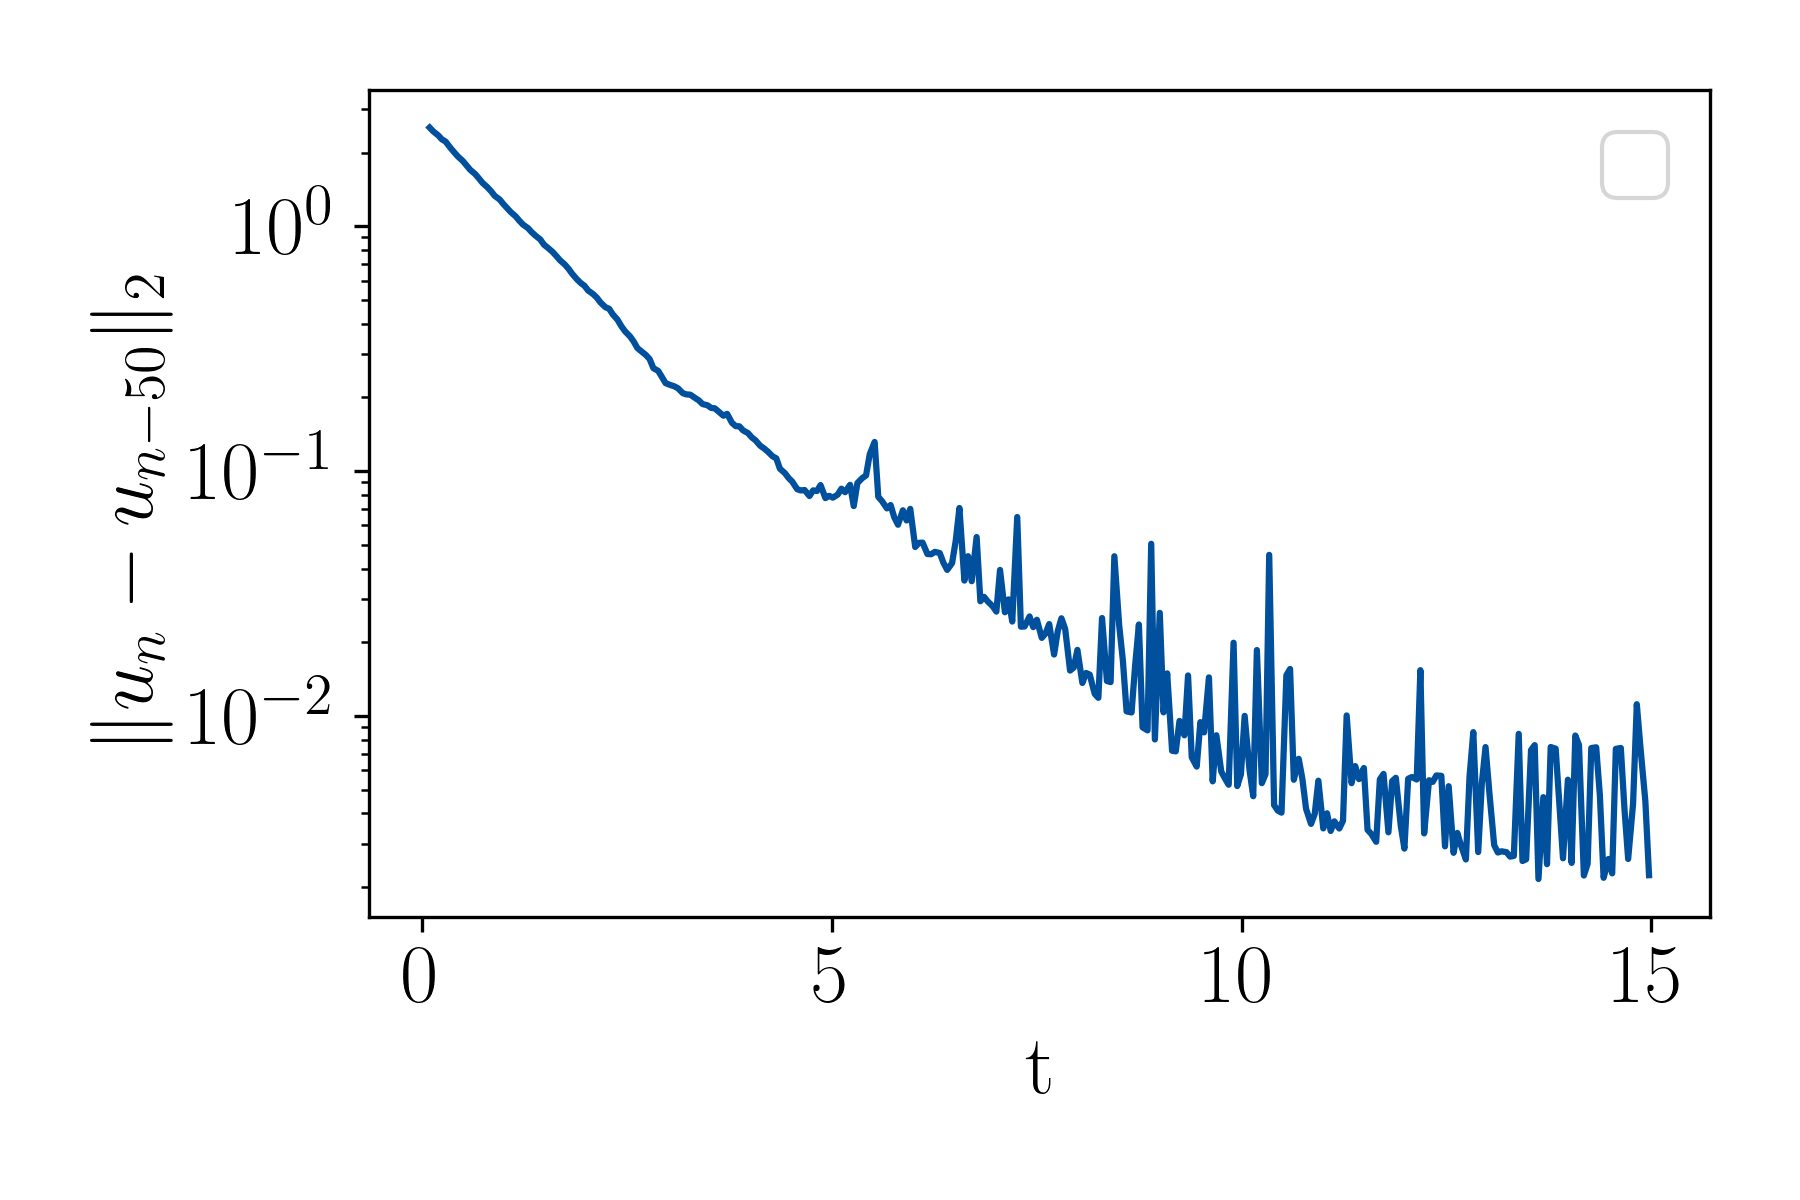
\includegraphics[height=3.5cm]{figures/Results/Many-points/model1/many_a99_res}%
}
\end{center}
\vspace{-2.5em}
\caption[Model 1 - Irregular and dense point set, $\alpha=0.99$]{Model 1: $h=0.01$, $9$ level curves, $\alpha=0.99$, $r_0=0.9$, reinitialize every $50$ steps}
\label{fig:m1-manypoints-a99}
\end{figure}

To obtain a better approximation, we increase $\alpha$ to $\alpha=0.999$ in the simulation displayed in \figref{fig:m1-manypoints-a999}. For the final contour for that parameter choice, we see a much closer approximation to the point set, only deviating at the sharpest corners. We also observe an interesting detail up in the right corner again. What was earlier a straight line, is now much more wavy and the reason is obvious. When the curve is now forced to go through all points, the curvature also needs to be zero at the points, meaning straight lines. Then the curvature must increase between the points reach them all. 
\begin{figure}
\begin{center}
\resizebox{.99\textwidth}{!}{%
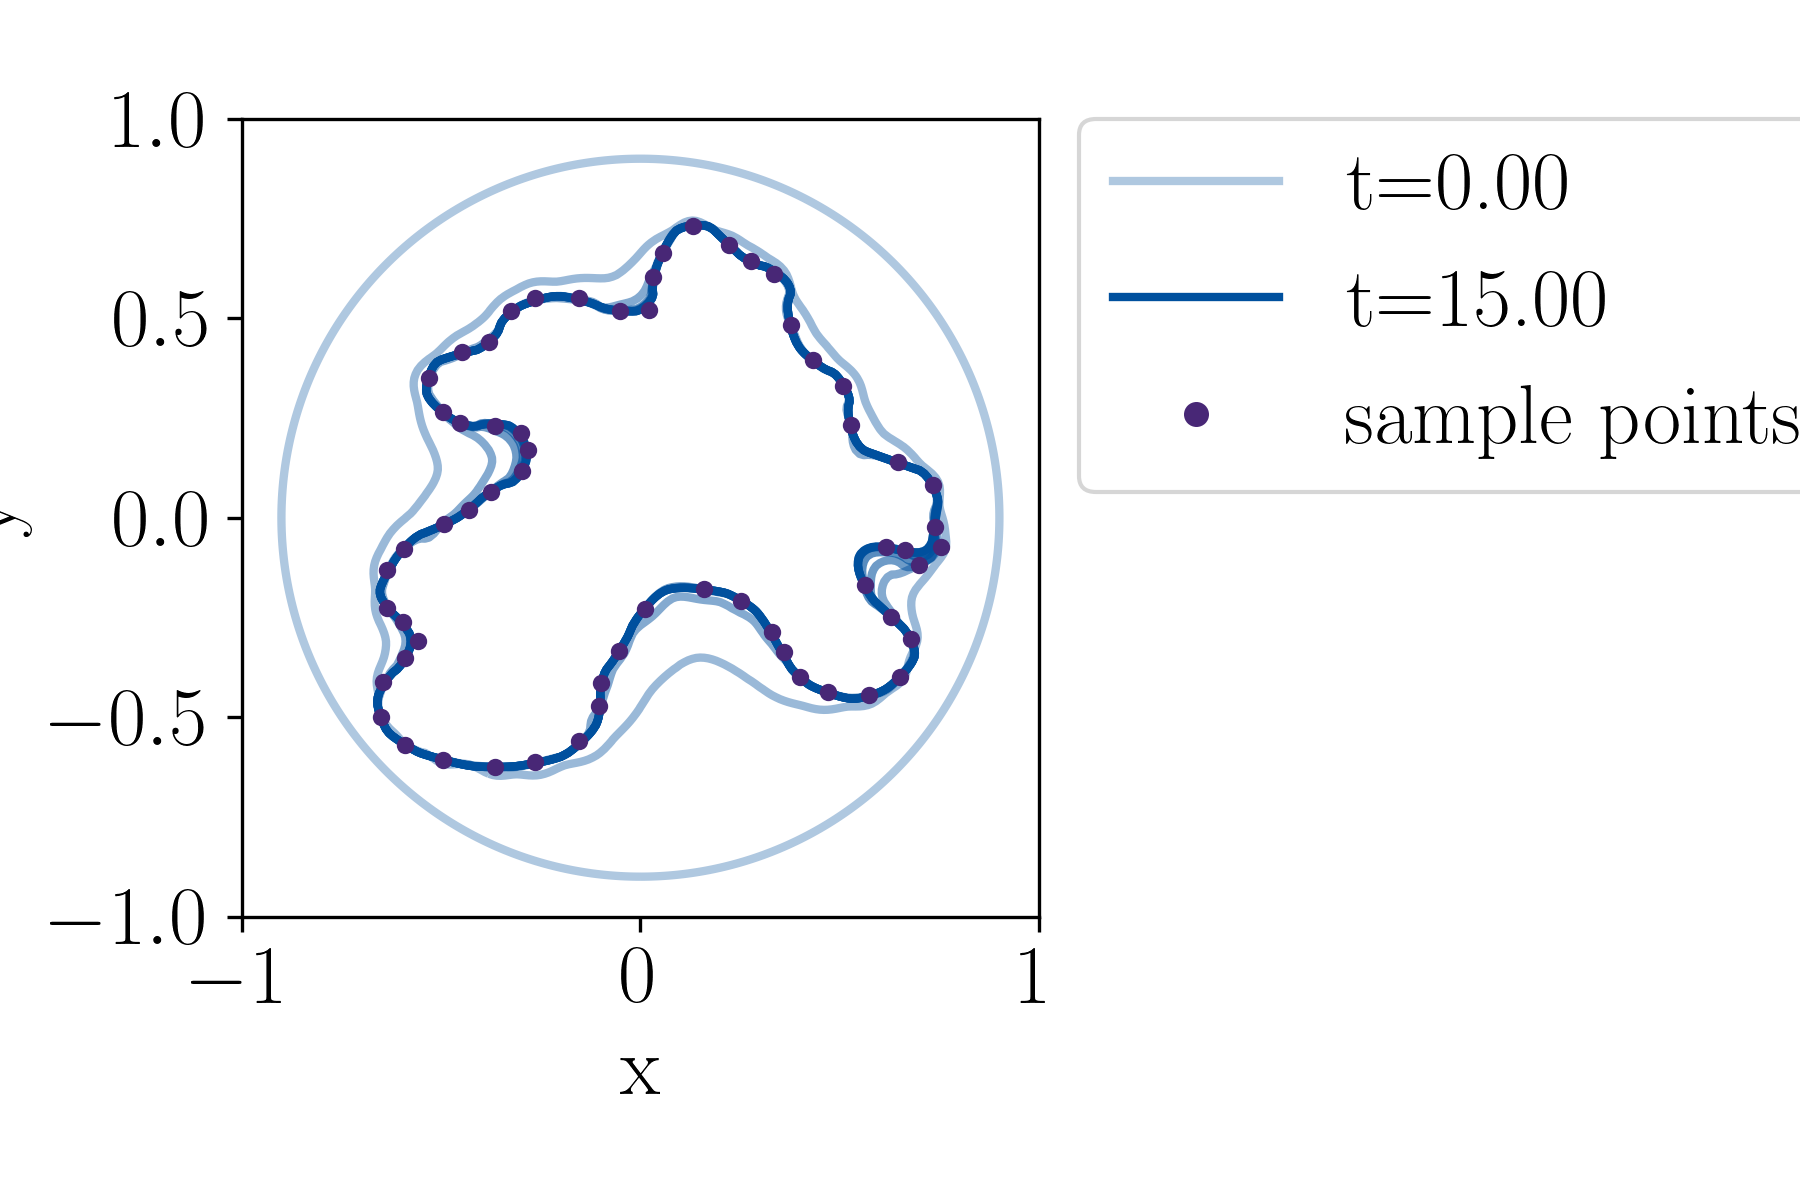
\includegraphics[height=3.5cm]{figures/Results/Many-points/model1/manypoints-a999.png}%
\,
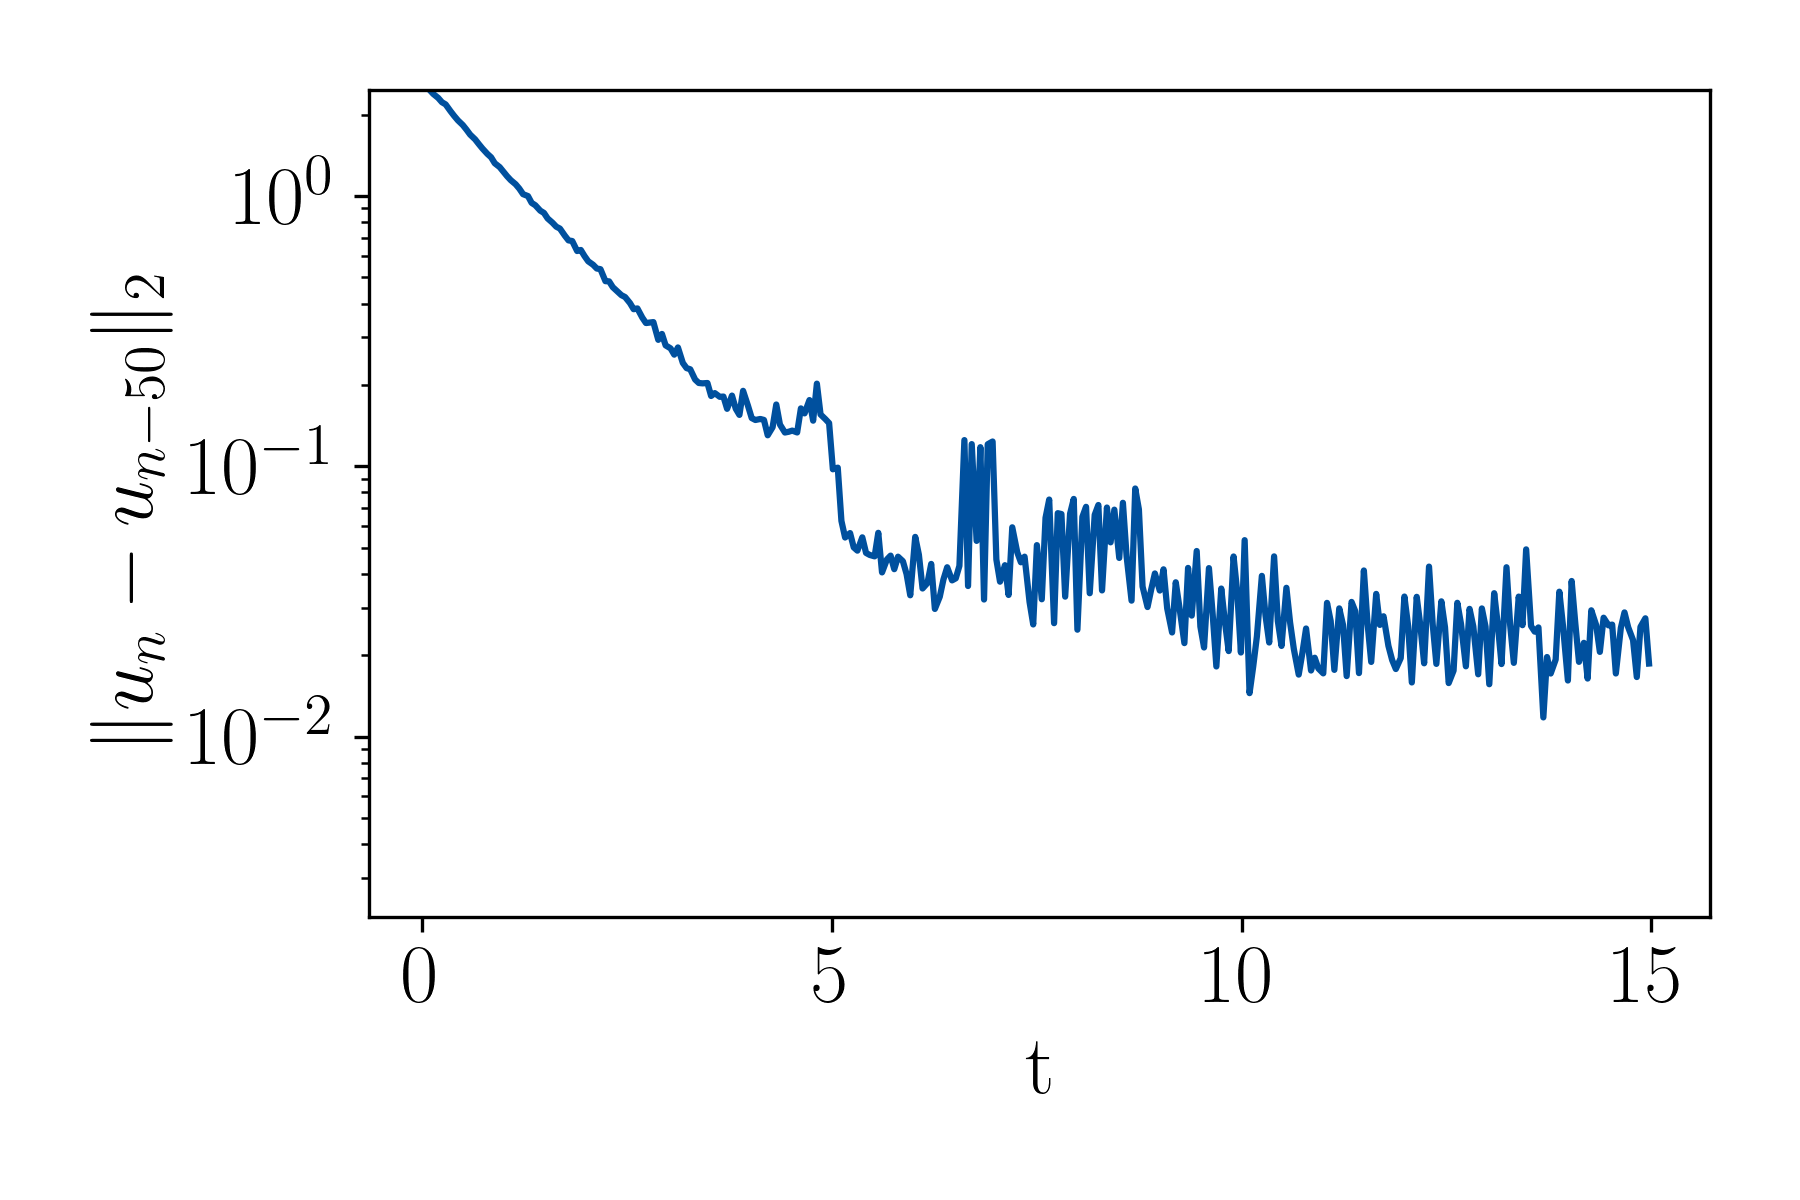
\includegraphics[height=3.5cm]{figures/Results/Many-points/model1/many_a999_res}%
}
\end{center}
\vspace{-2.5em}
\caption[Model 1 - Irregular and dense point set, $\alpha=0.999$]{Model 1: $h=0.01$, $9$ level curves, $\alpha=0.999$, $r_0=0.9$, reinitialize every $50$ steps}
\label{fig:m1-manypoints-a999}
\end{figure}

The residual plots for in \figref{fig:m1-manypoints-a99} and \figref{fig:m1-manypoints-a999} shows that both curves have a small velocity compared to what we have seen for many of the oscillating models, but we do not see the nice convergence as in \figref{fig:model1-sigma-dist-full}. We also observe that the model where the curvature is more dominant has a smaller velocity in the final curve. This seems natural because when the distance dominates, the curve can easily be drawn back and forth over the points, but the curvature draws only in the inward direction. Thus it makes sense that we observe less oscillations for smaller $\alpha$. 


\begin{figure}
\begin{center}
\resizebox{.99\textwidth}{!}{%
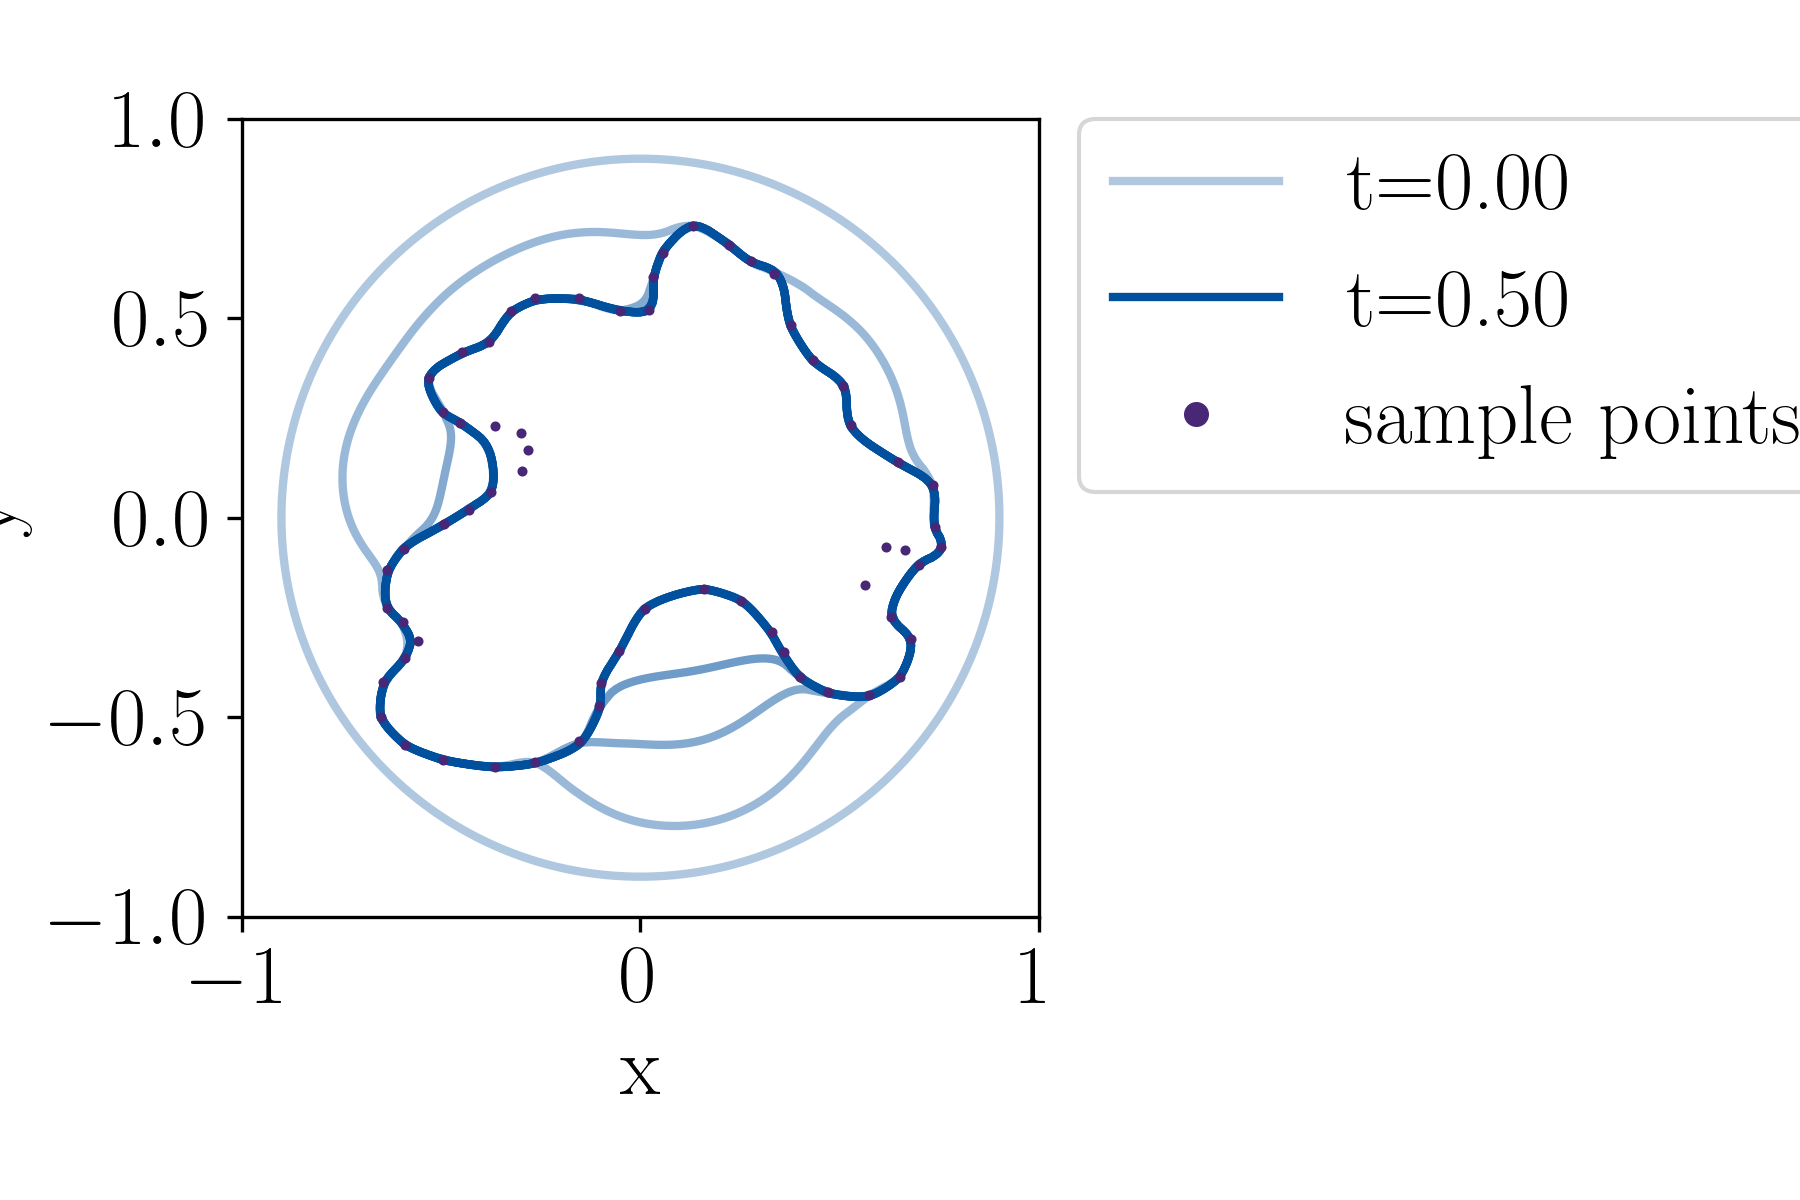
\includegraphics[height=3.5cm]{figures/Results/Many-points/model2/manypoints-a04.png}%
\,
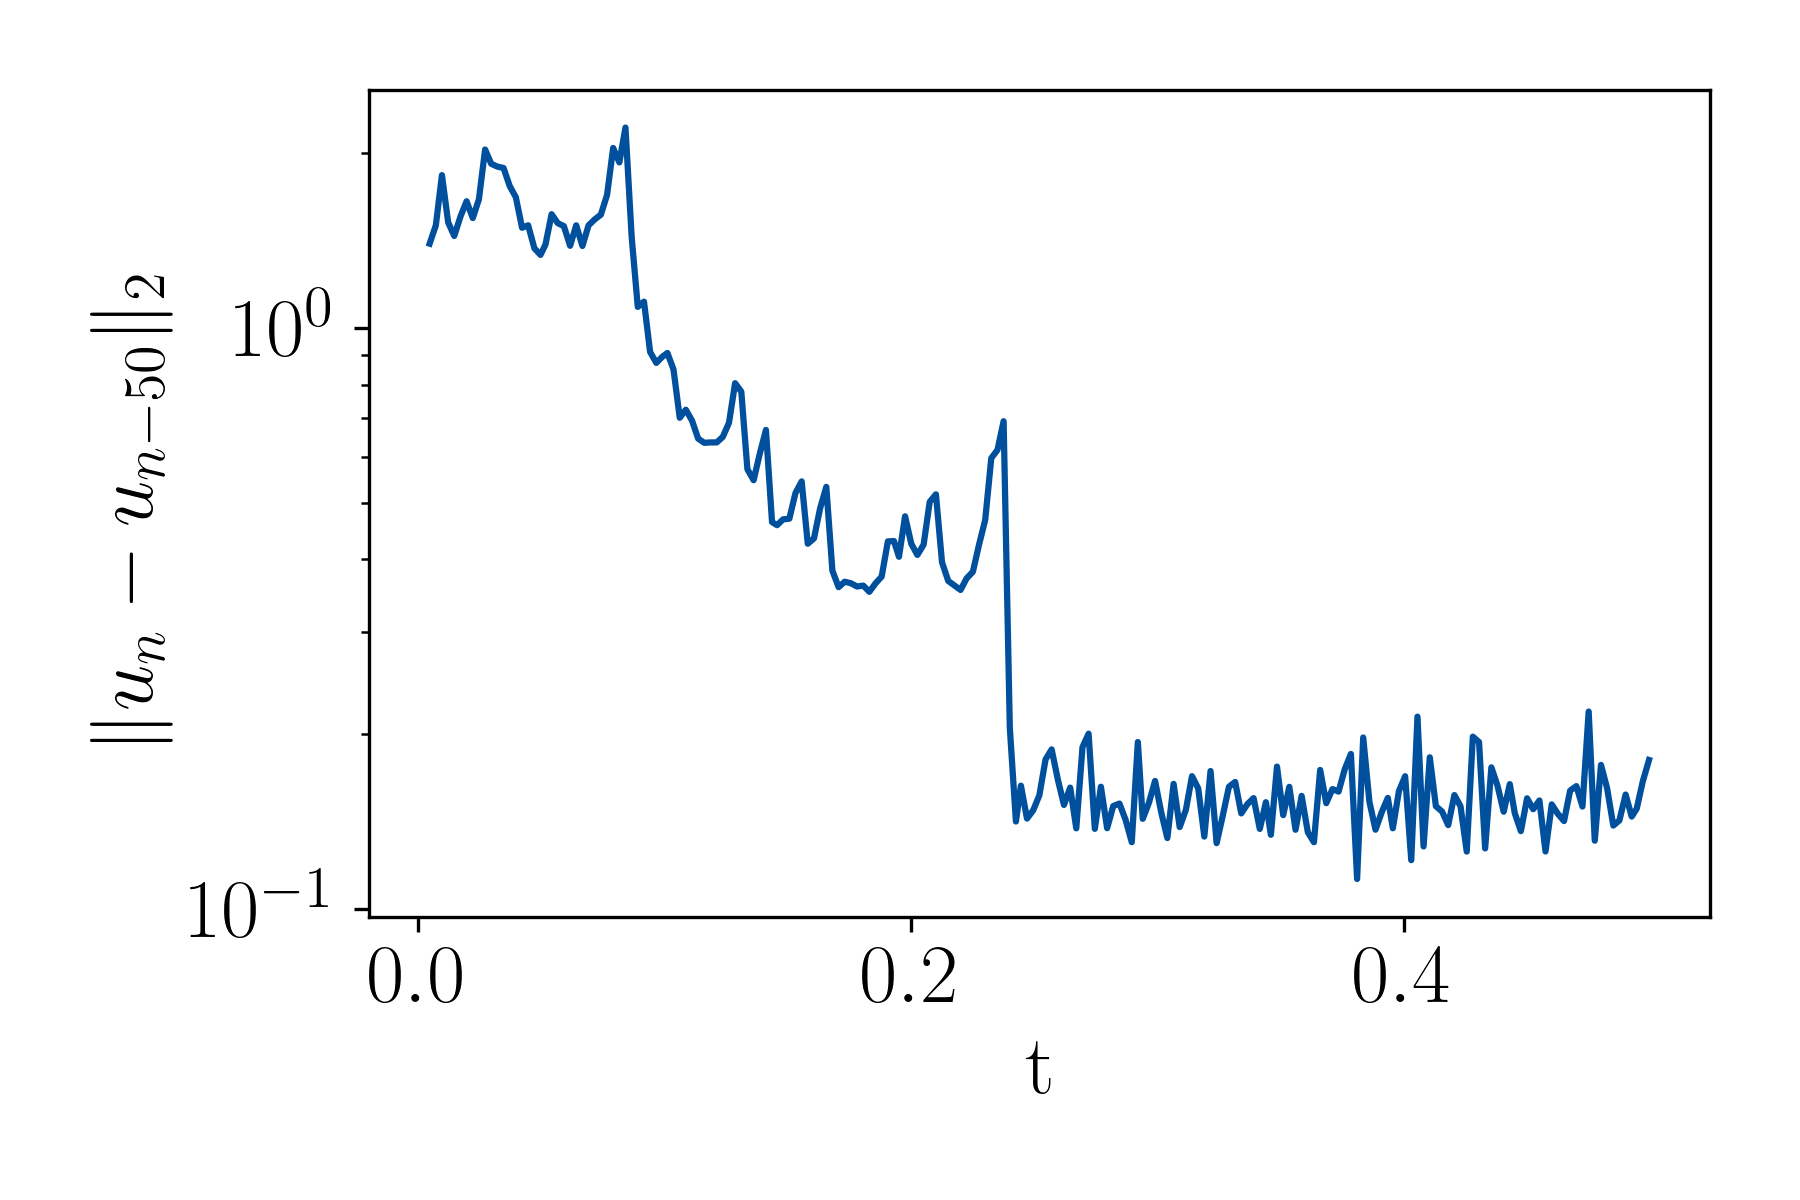
\includegraphics[height=3.5cm]{figures/Results/Many-points/model2/many-a04-logy.png}%
}
\end{center}
\vspace{-2.5em}
\caption[Model 2 - Irregular and dense point set $\beta=1$]{Model 2: $h=0.01$, $9$ level curves, $\alpha=0.4$, $r_0=0.9$, reinitialize every $50$ steps, $\delta=10^{-2}$}
\label{fig:m2-manypoints-a04}
\end{figure}

\begin{figure}
\begin{center}
\resizebox{.99\textwidth}{!}{%
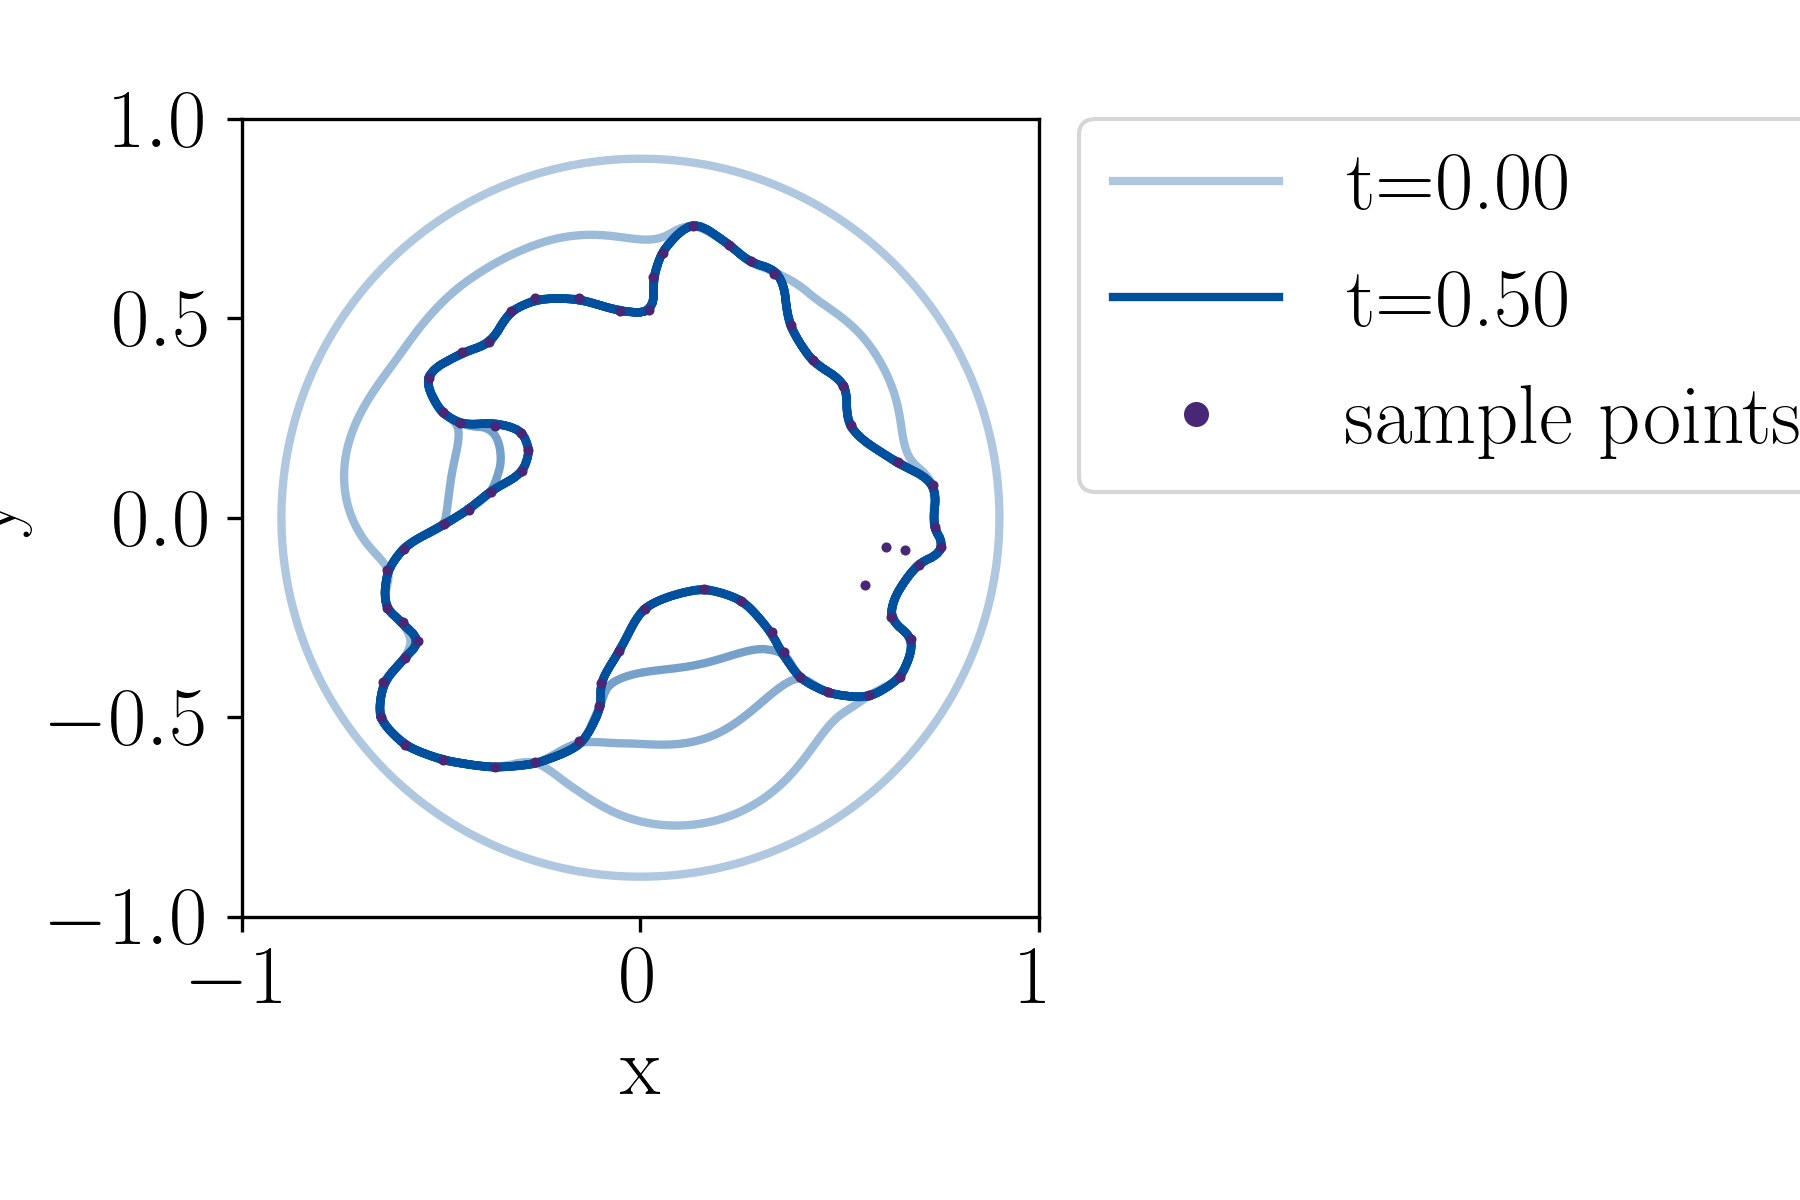
\includegraphics[height=3.5cm]{figures/Results/Many-points/model2/many-d1-a4-b08-t1.png}%
\,
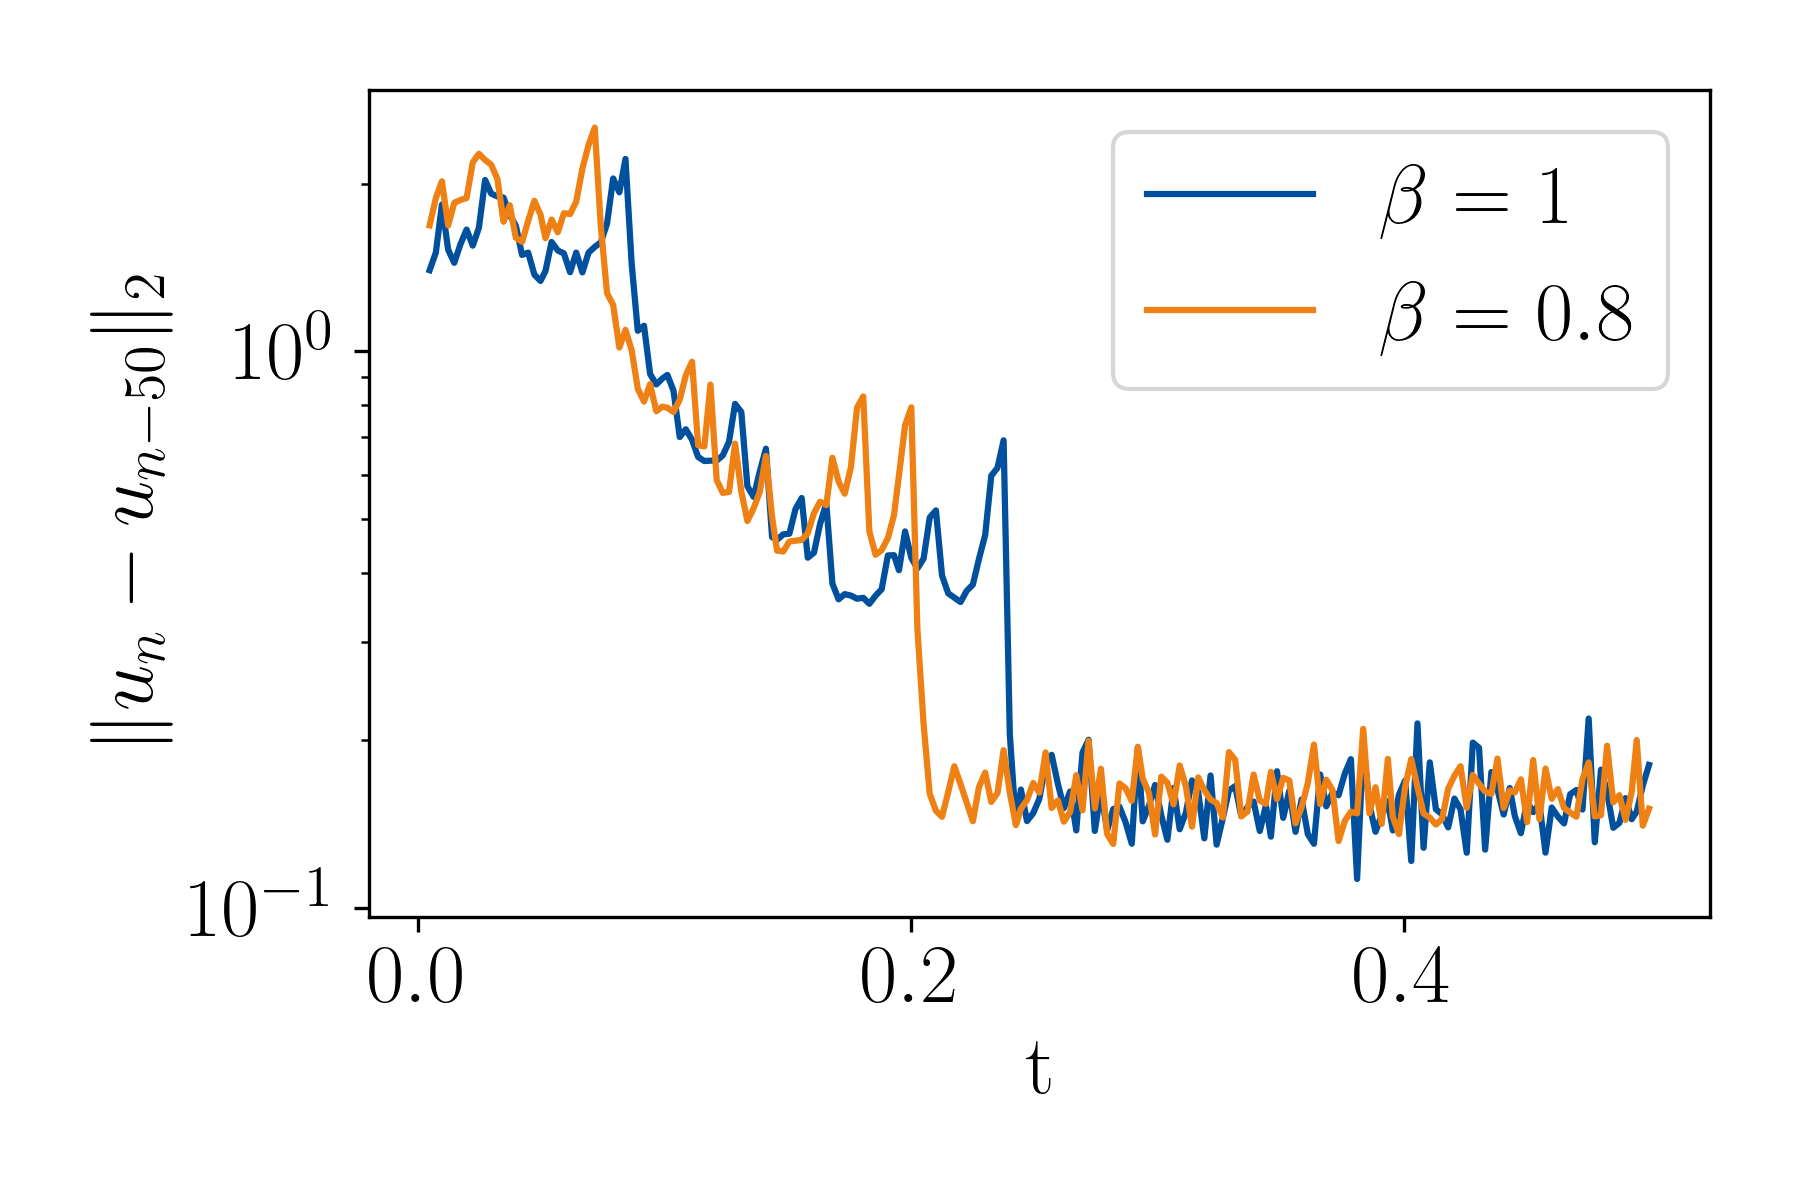
\includegraphics[height=3.5cm]{figures/Results/Many-points/model2/many_d1_b1_b08_res.png}%
}
\end{center}
\vspace{-2.5em}
\caption[Model 2 - Irregular and dense point set $\beta=0.8$]{Model 2: $h=0.01$, $9$ level curves, $\alpha=0.4$, $r_0=0.9$, reinitialize every $50$ steps, $\delta=10^{-2}$, $\beta=0.8$}
\label{fig:m2-manypoints-b08}
\end{figure}

We see in \figref{fig:m2-manypoints-a04} that the level curves are more glued to the sample points for model 2 again, and it is interesting that even where the curve do not cover the points, it does not move around visibly. It seems like the curve is not attracted enough to the point set at that distance. We try to mend this by scaling with the term $\beta$ to $\beta=0.8$. This should mean that the inverse distance is still bounded by $\delta$, but it should have more effect further from the point set. We see the result in \figref{fig:m2-manypoints-b08}, and we do see a difference. Up in the left corner, the distance term has attracted the curve to the sample points, but we do not see this in the lower right corner. 

Further, if we compare the shape of the final curve in \figref{fig:m2-manypoints-a04} compared to the final curve for model 1 in \figref{fig:m1-manypoints-a999}, we see that the shape is slightly different also where both covers the point set. Model 1 is actually more wavy in the top right corner which could be surprising because model 1 has been smoother up until now. If we look really close, we see that the curve is much smoother around the sample points for model 1, but to obtain such small curvature at the points, the curve do not take the shortest paths between the points. The curve in model 2 is on the other hand much more similar to the shortest path between.


We take a look at model 3, we see in the \figref{fig:m3-manypoints-a09} and \figref{fig:m3-many-points-b1-b2} that it is changing the parameter $\alpha$ that has the biggest effect. In \figref{fig:m3-many-points-b1-b2} $\beta=1$ to the left and $\beta=2$ to the right, and the only visible difference is the density of the contours in the beginning, which is also visible in the residual plot in \figref{fig:m3-manypoints-a09}. We here see that $\beta=1$ provides a solution which reaches its final state before $\beta=2$ without yielding a worse solution.

\begin{figure}
\begin{center}
\resizebox{.99\textwidth}{!}{%
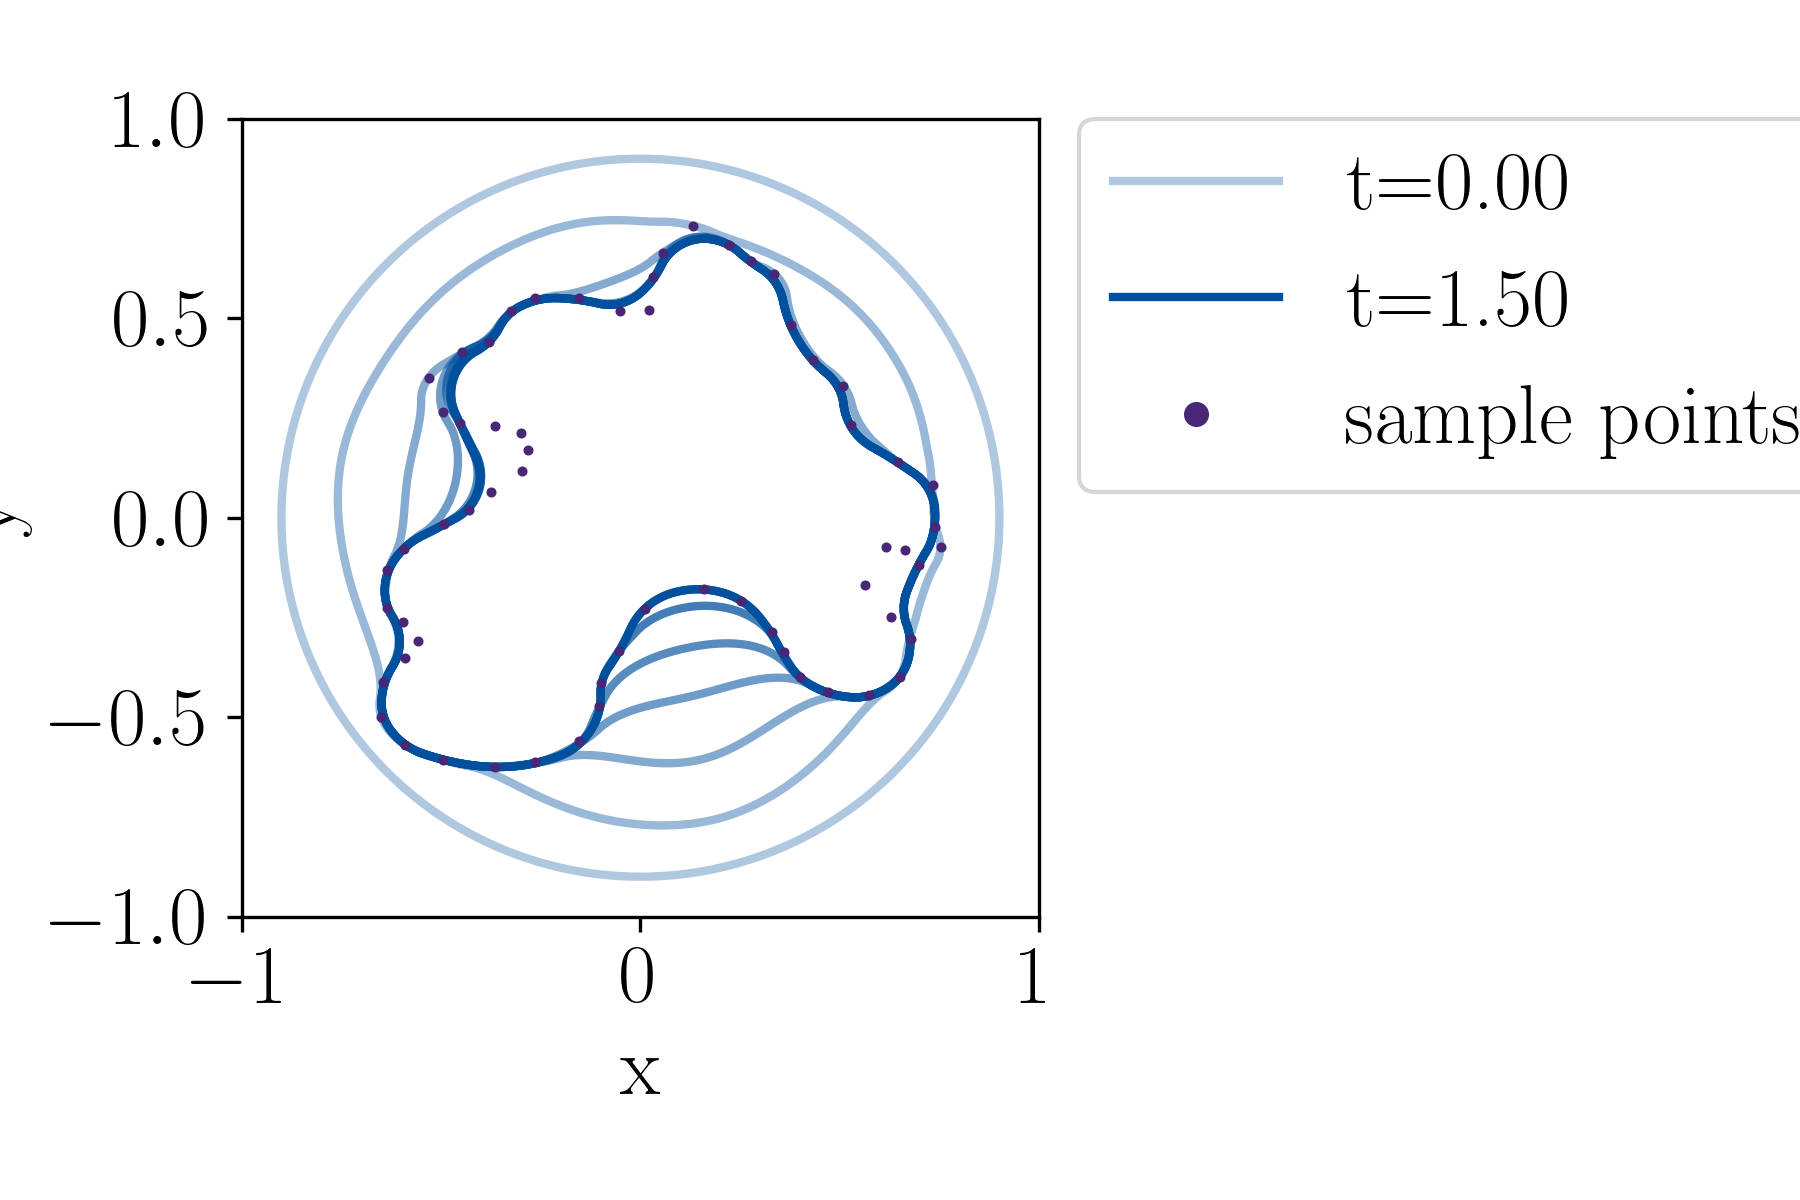
\includegraphics[height=3.5cm]{figures/Results/Many-points/model3/manypoints-a09.png}%
\,
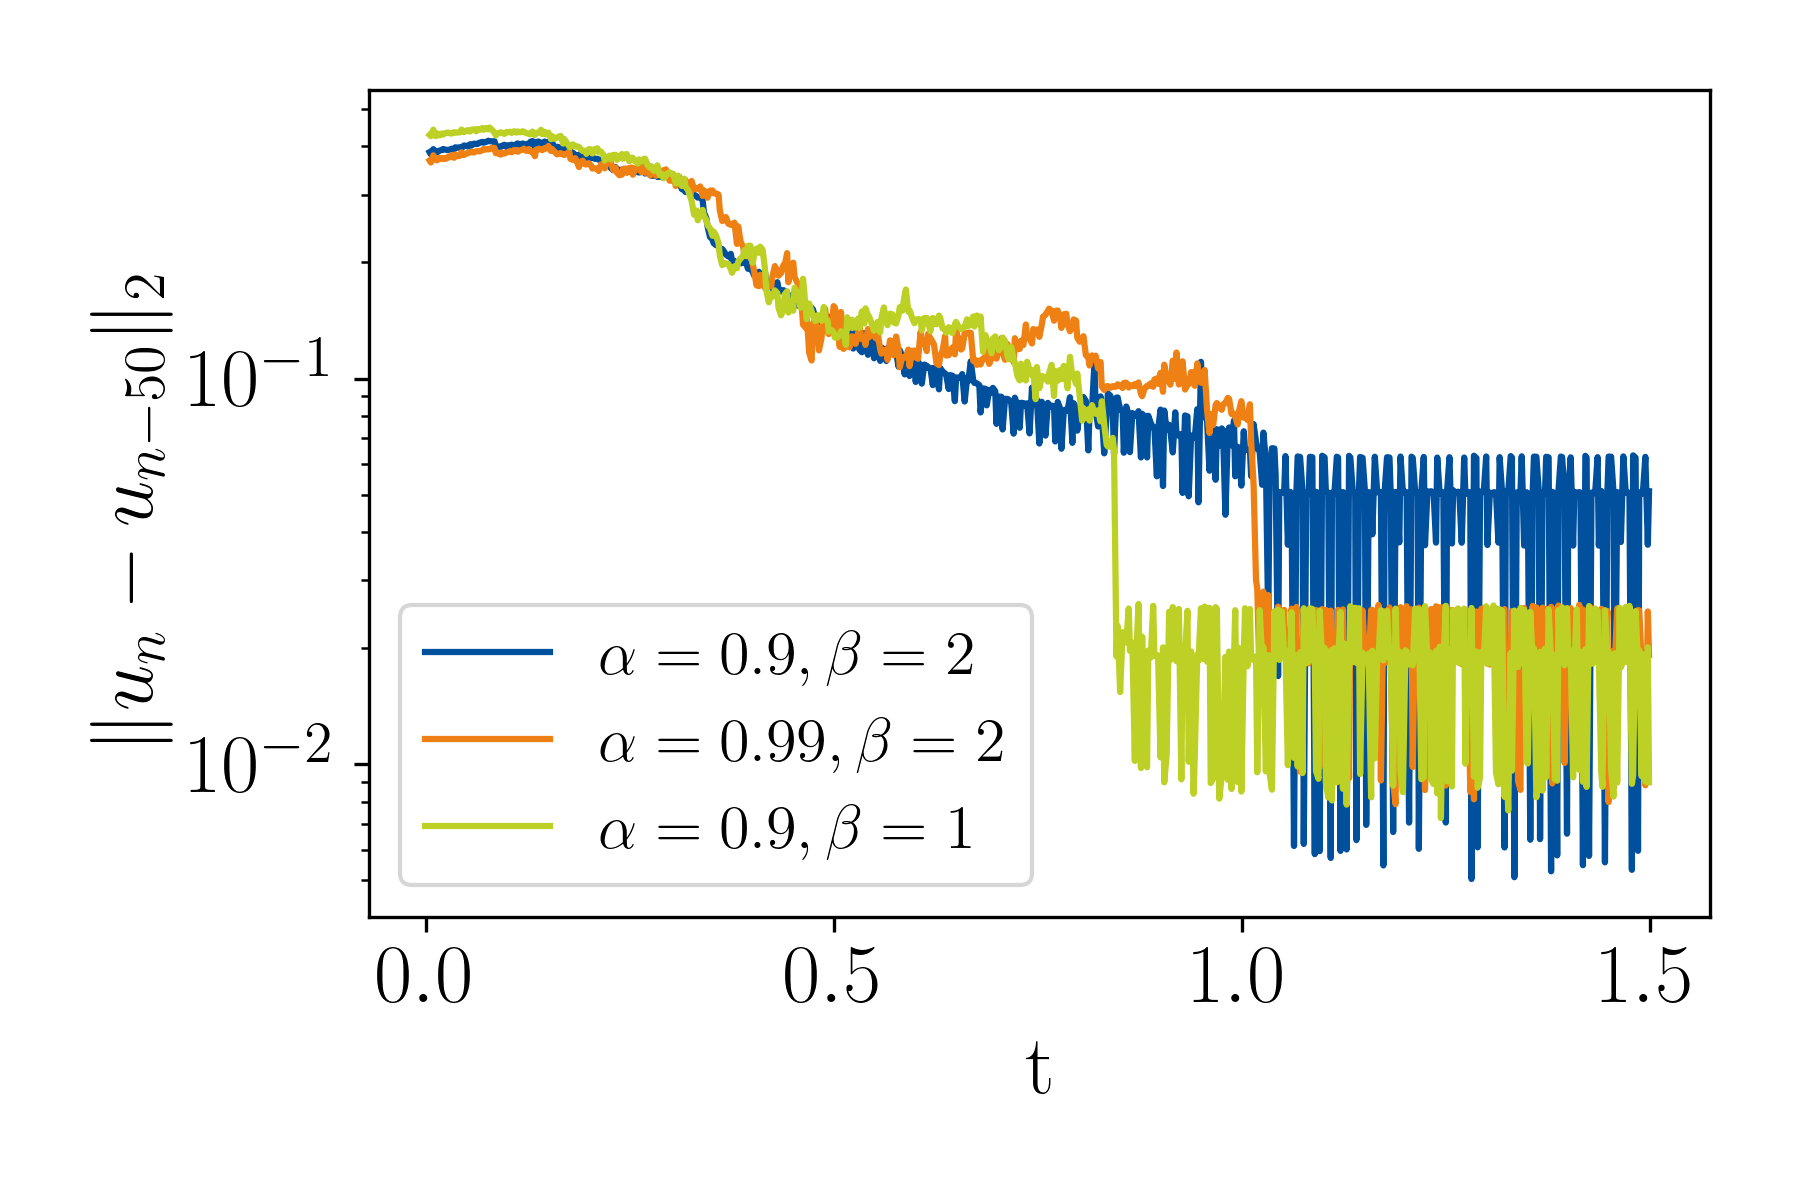
\includegraphics[height=3.5cm]{figures/Results/Many-points/model3/many-a09-a099-res.png}%
}
\end{center}
\vspace{-2.5em}
\caption[Model 3 - Irregular and dense point set $\alpha =0.9$]{Model 3: $h=0.01$, $9$ level curves, $\alpha=0.9$, $r_0=0.9$, reinitialize every $50$ steps, $\beta=2$}
\label{fig:m3-manypoints-a09}
\end{figure}

\begin{figure}
\begin{center}
\resizebox{.99\textwidth}{!}{%
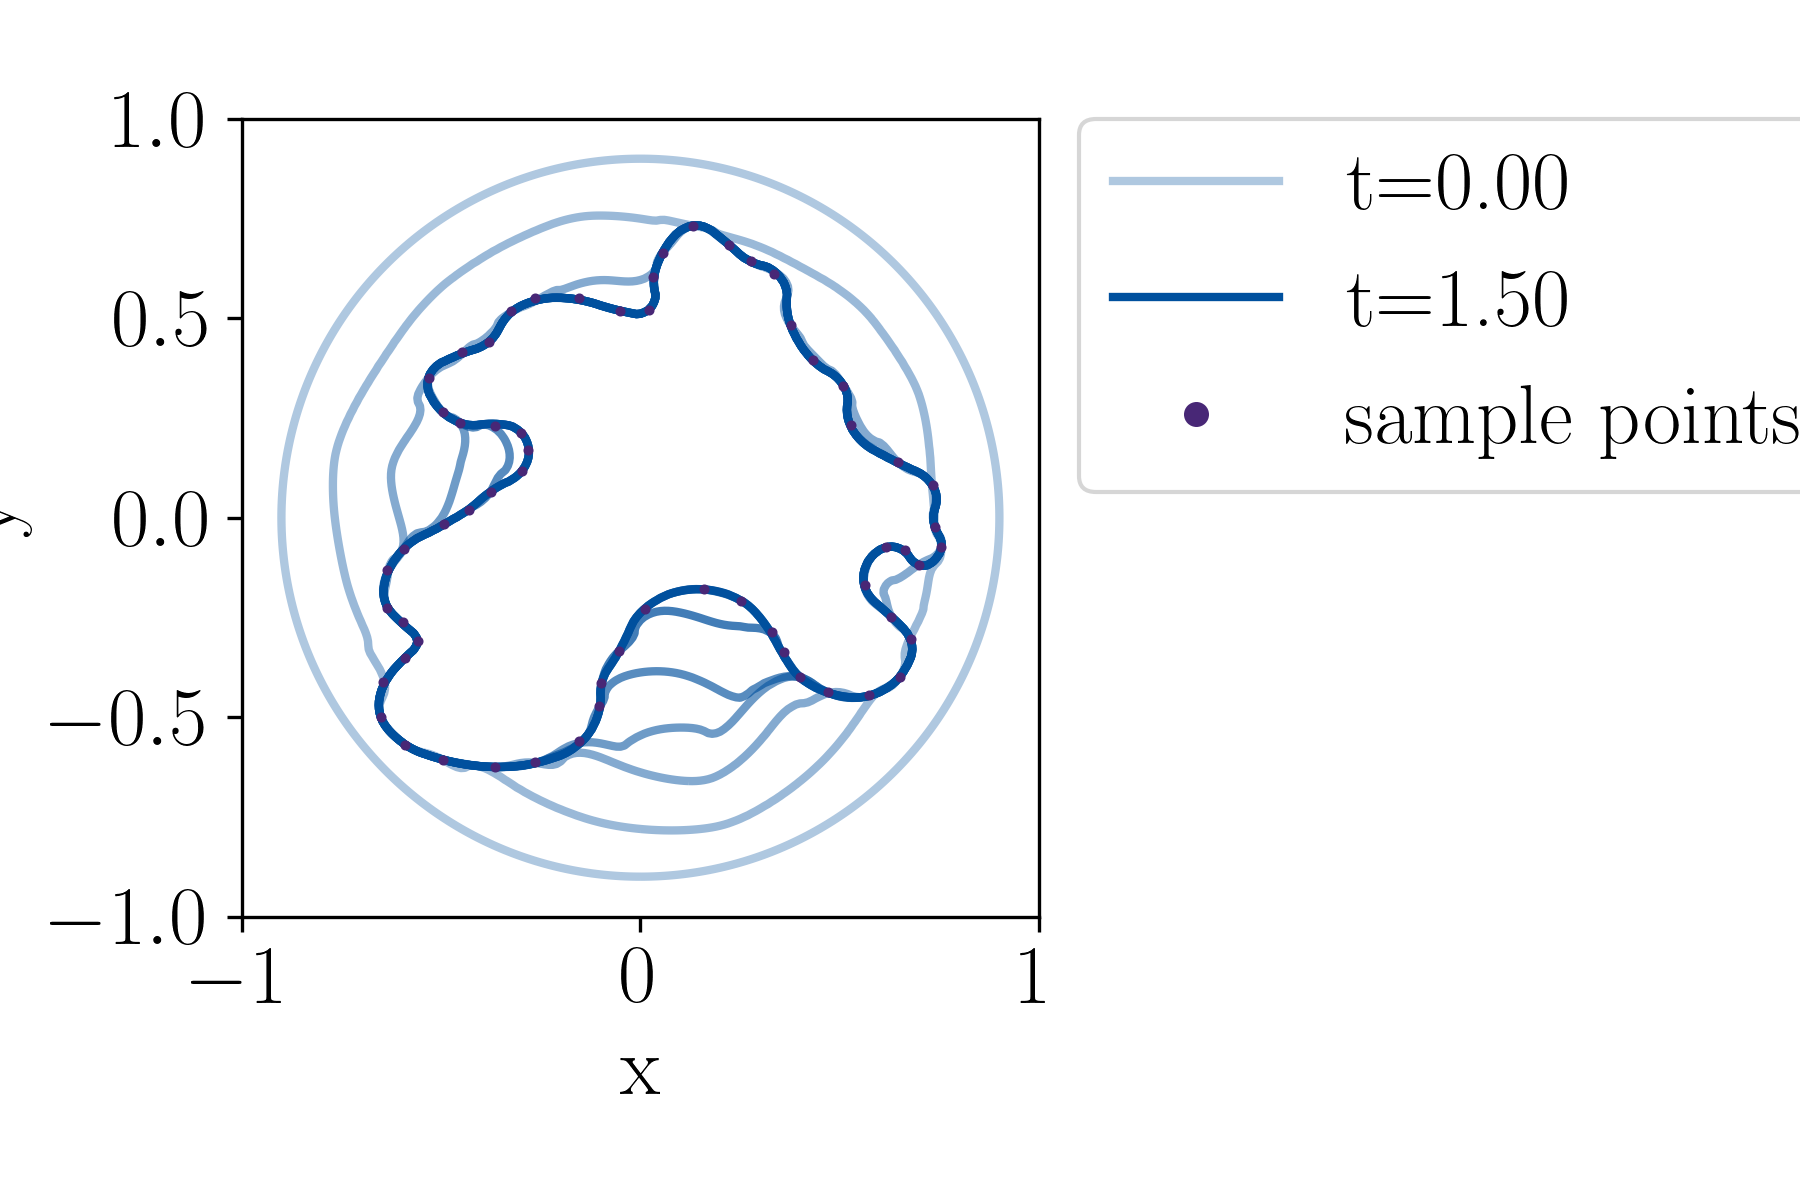
\includegraphics[height=3.5cm]{figures/Results/Many-points/model3/manypoints-a099.png}%
\,
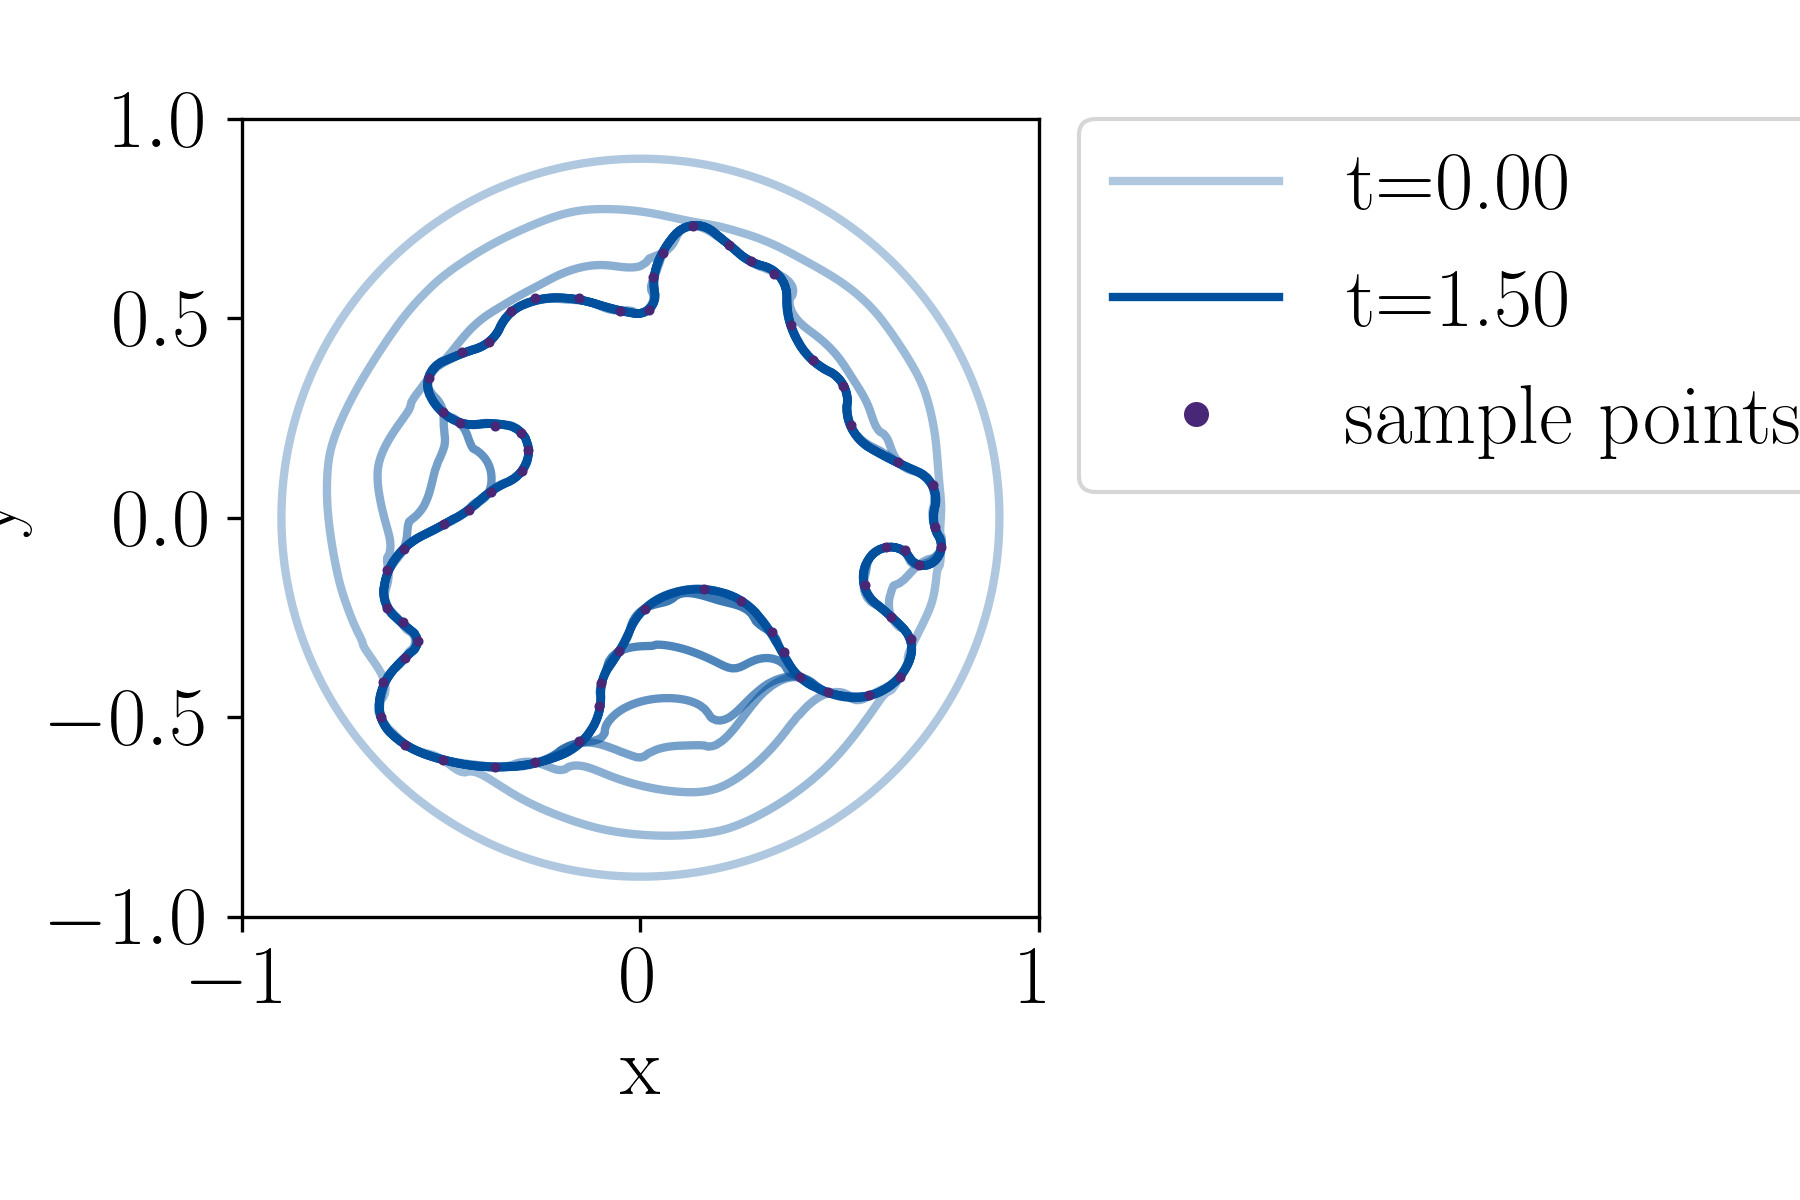
\includegraphics[height=3.5cm]{figures/Results/Many-points/model3/many-a99-b2.png}%
}
\end{center}
\vspace{-2.5em}
\caption[Model 3 - Irregular and dense point set $\beta$ parameter]{Model 3: $h=0.01$, $9$ level curves, $\alpha=0.99$, $r_0=0.9$, reinitialize every $50$ steps, $\beta=2$}
\label{fig:m3-many-points-b1-b2}
\end{figure}



\clearpage
\section{Test Case 4: Noisy Data}
The noisy data set is the test case closest to the description in the objective of the thesis, so it will be very interesting to see how the models preform. Here, we look for a smooth curve, which captures the shape while being distracted as little as possible by the noise. 

This should be the perfect example for model 1, since the curvature plays a bigger role when the distance is small, which should yield a smoother curve close to the point set. We also see this in \figref{fig:m1-noisypoints-a99}, where the shape of the circle is captured very well and the curve is rather smooth. What we also observe is that the curve is located on the inside of the noisy band of points rather than in the middle. From what we saw from the circle example, this could be mended by tuning up the parameter $\alpha$.

We did this in \figref{fig:m1-noisypoints-a999} and we can see that it forced the final curve more to the middle of the band of points. However, it is not as smooth for higher values of $\alpha$, which is also expected as the curvature is then less influential.

Another effect which we now observe in the residual plot in \figref{fig:m1-noisypoints-a99} is what can look like at least two solutions at $t\sim 7.5$ and $t\sim 11$, where the curve starts slowing down, before speeding up again. The reason for this behavior lies in the distribution of the sample points. The the times where the curve slows down, the relation between the curvature and distance is almost fulfilled, and the velocity is small. But since the curve is not still, it can move so long that the curve suddenly get a new point as its closest point and then the speed increases. 

\begin{figure}
\begin{center}
\resizebox{.99\textwidth}{!}{%
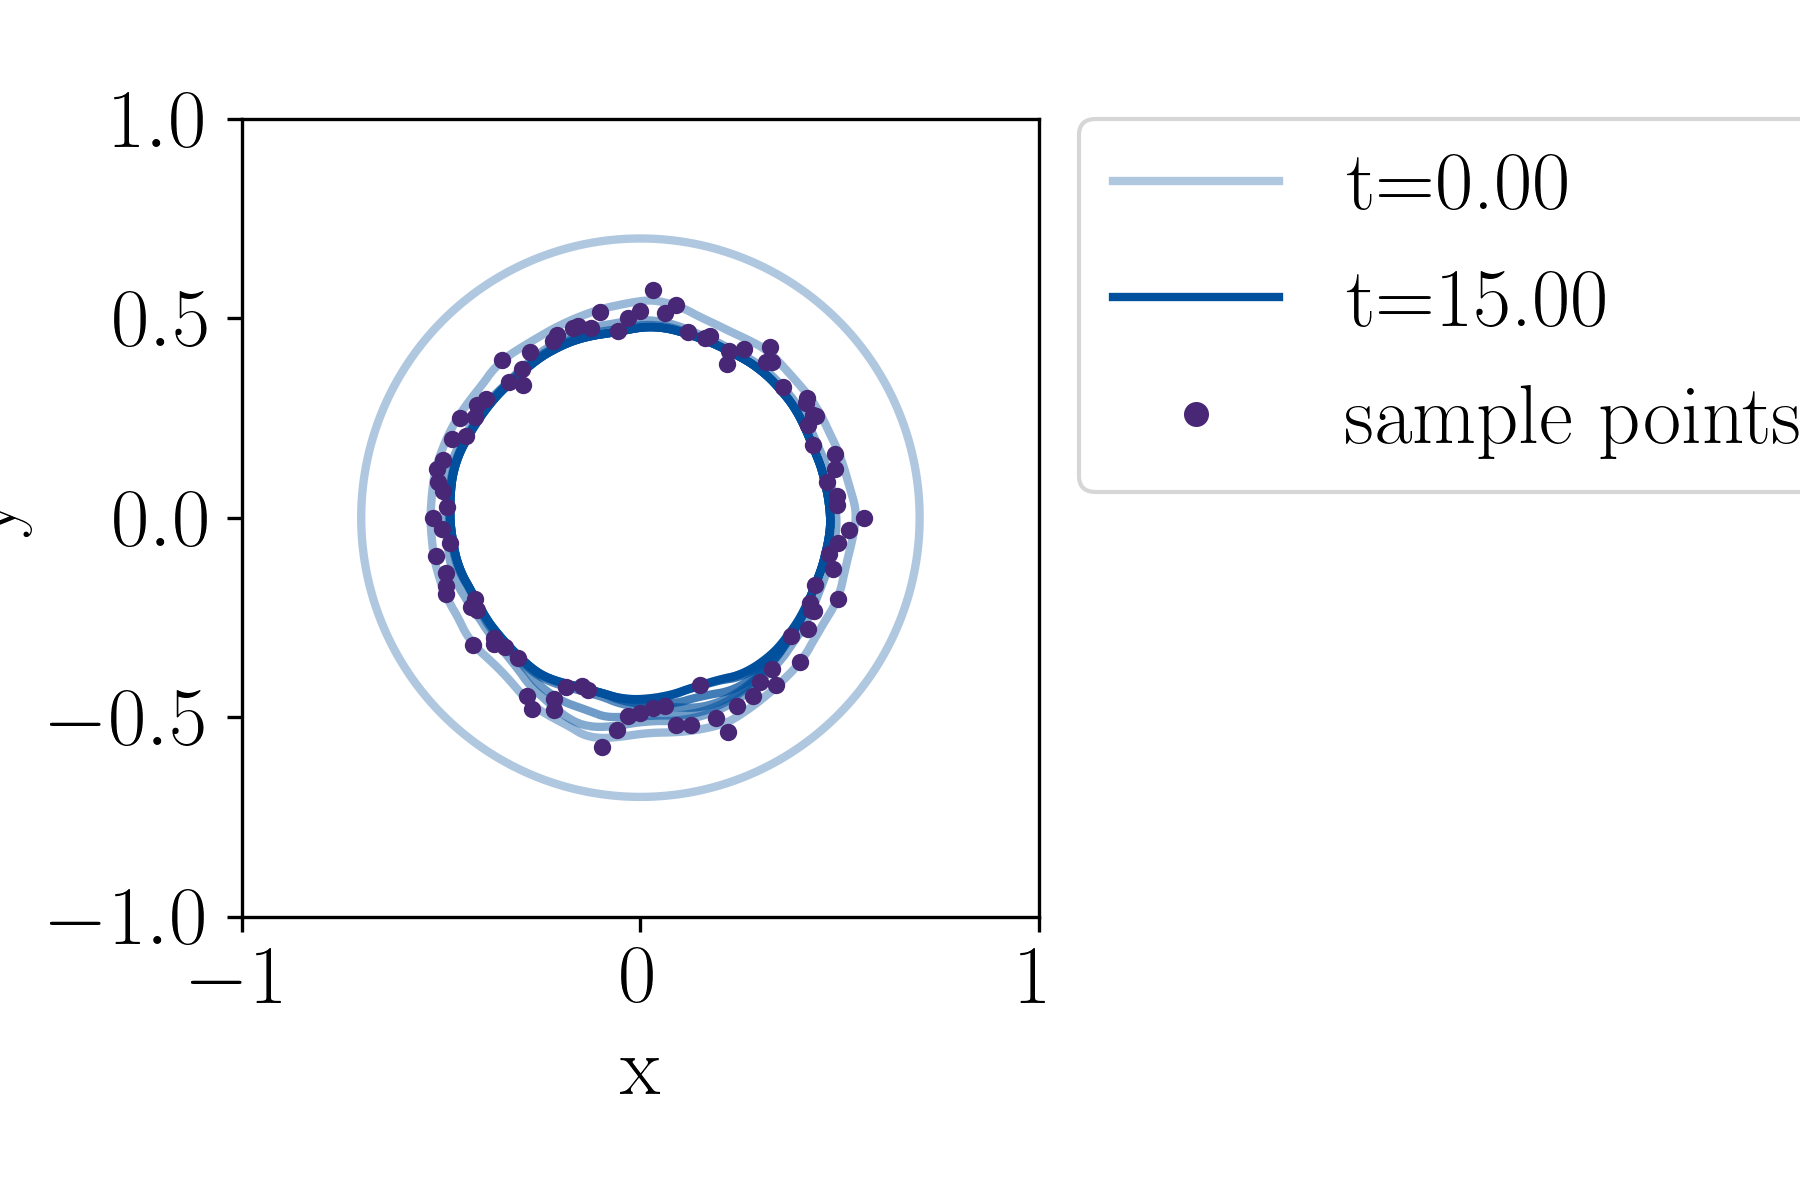
\includegraphics[height=3.5cm]{figures/Results/Noisy-points/model1/noisypoints-a99.png}%
\,
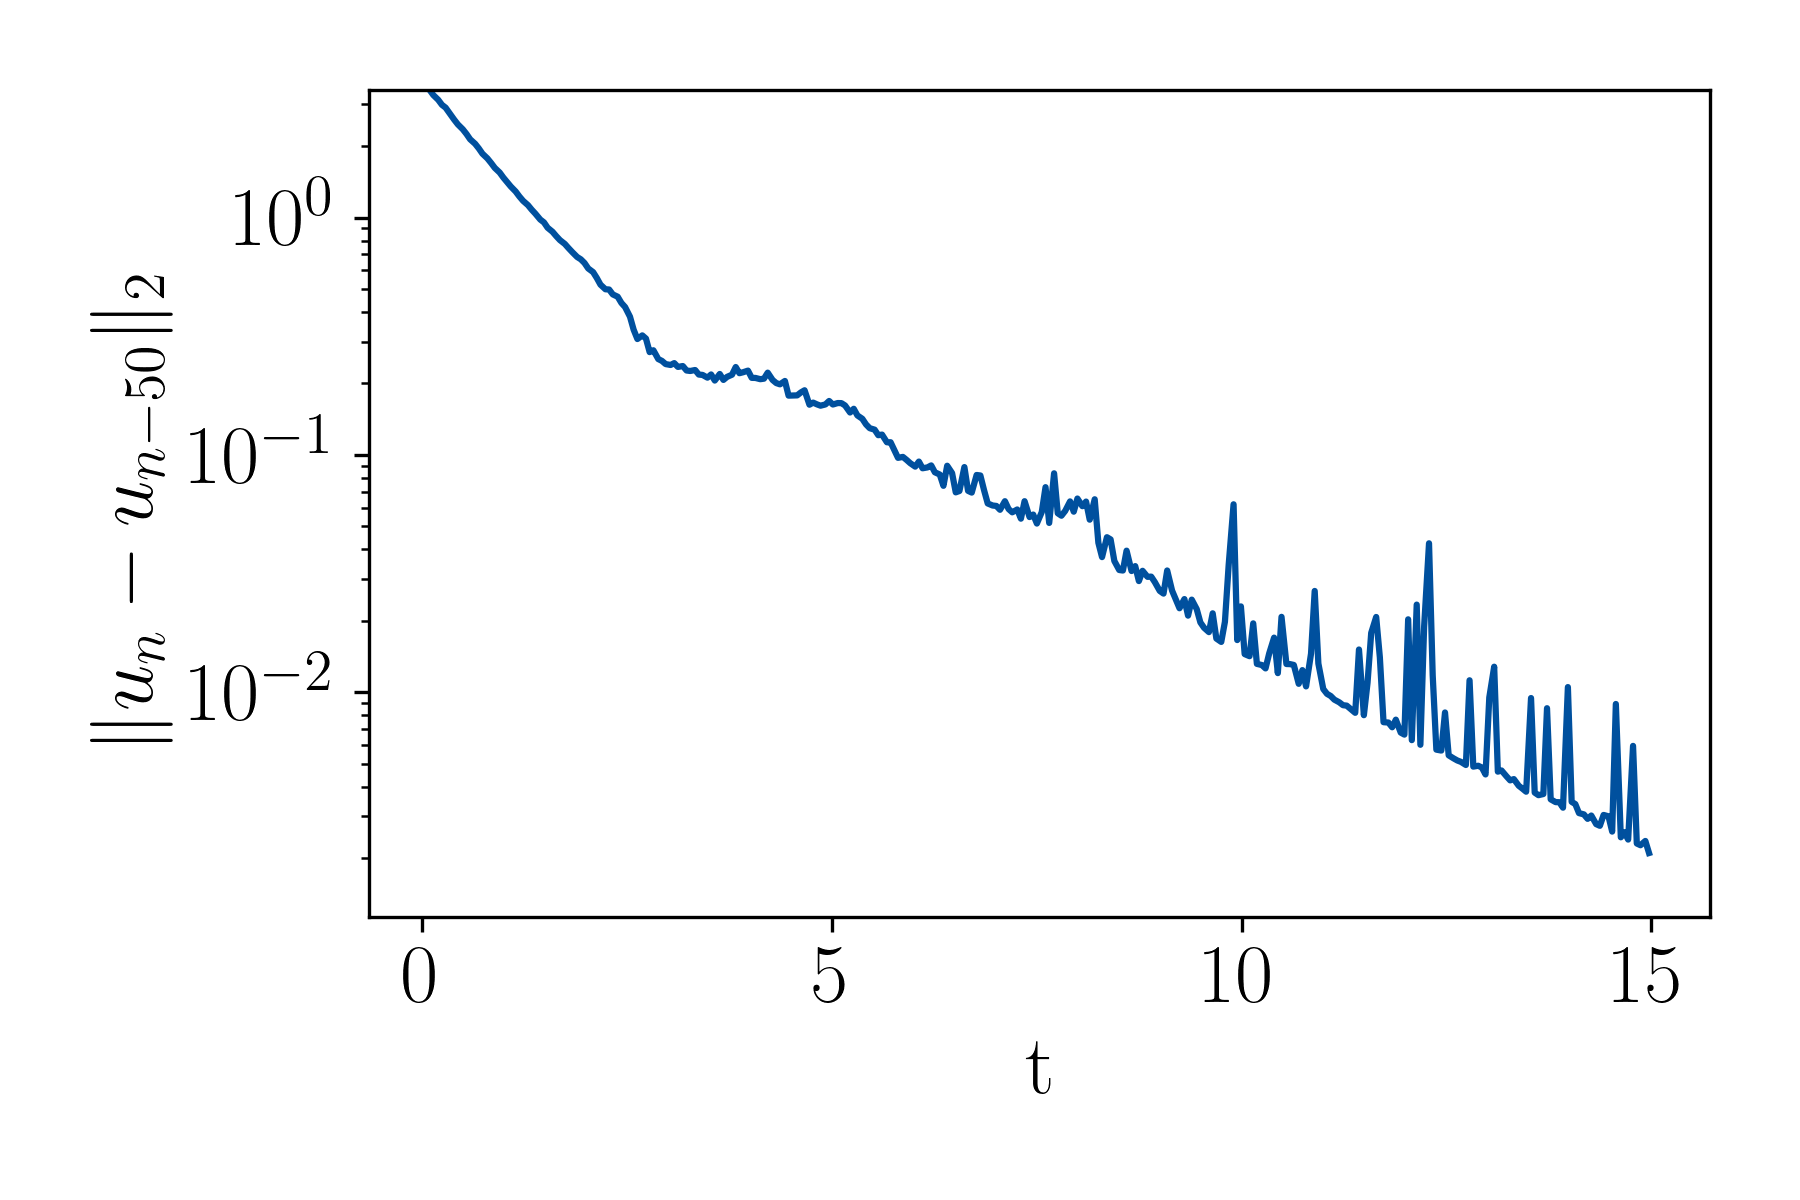
\includegraphics[height=3.5cm]{figures/Results/Noisy-points/model1/noisy-a99-res.png}%
}
\end{center}
\vspace{-2.5em}
\caption[Model 1 - Noisy point set, $\alpha=0.99$]{Model 1: $h=0.01$, $9$ level curves, $\alpha=0.99$, $r_0=0.9$, reinitialize every $50$ steps}
\label{fig:m1-noisypoints-a99}
\end{figure}

\begin{figure}
\begin{center}
\resizebox{.99\textwidth}{!}{%
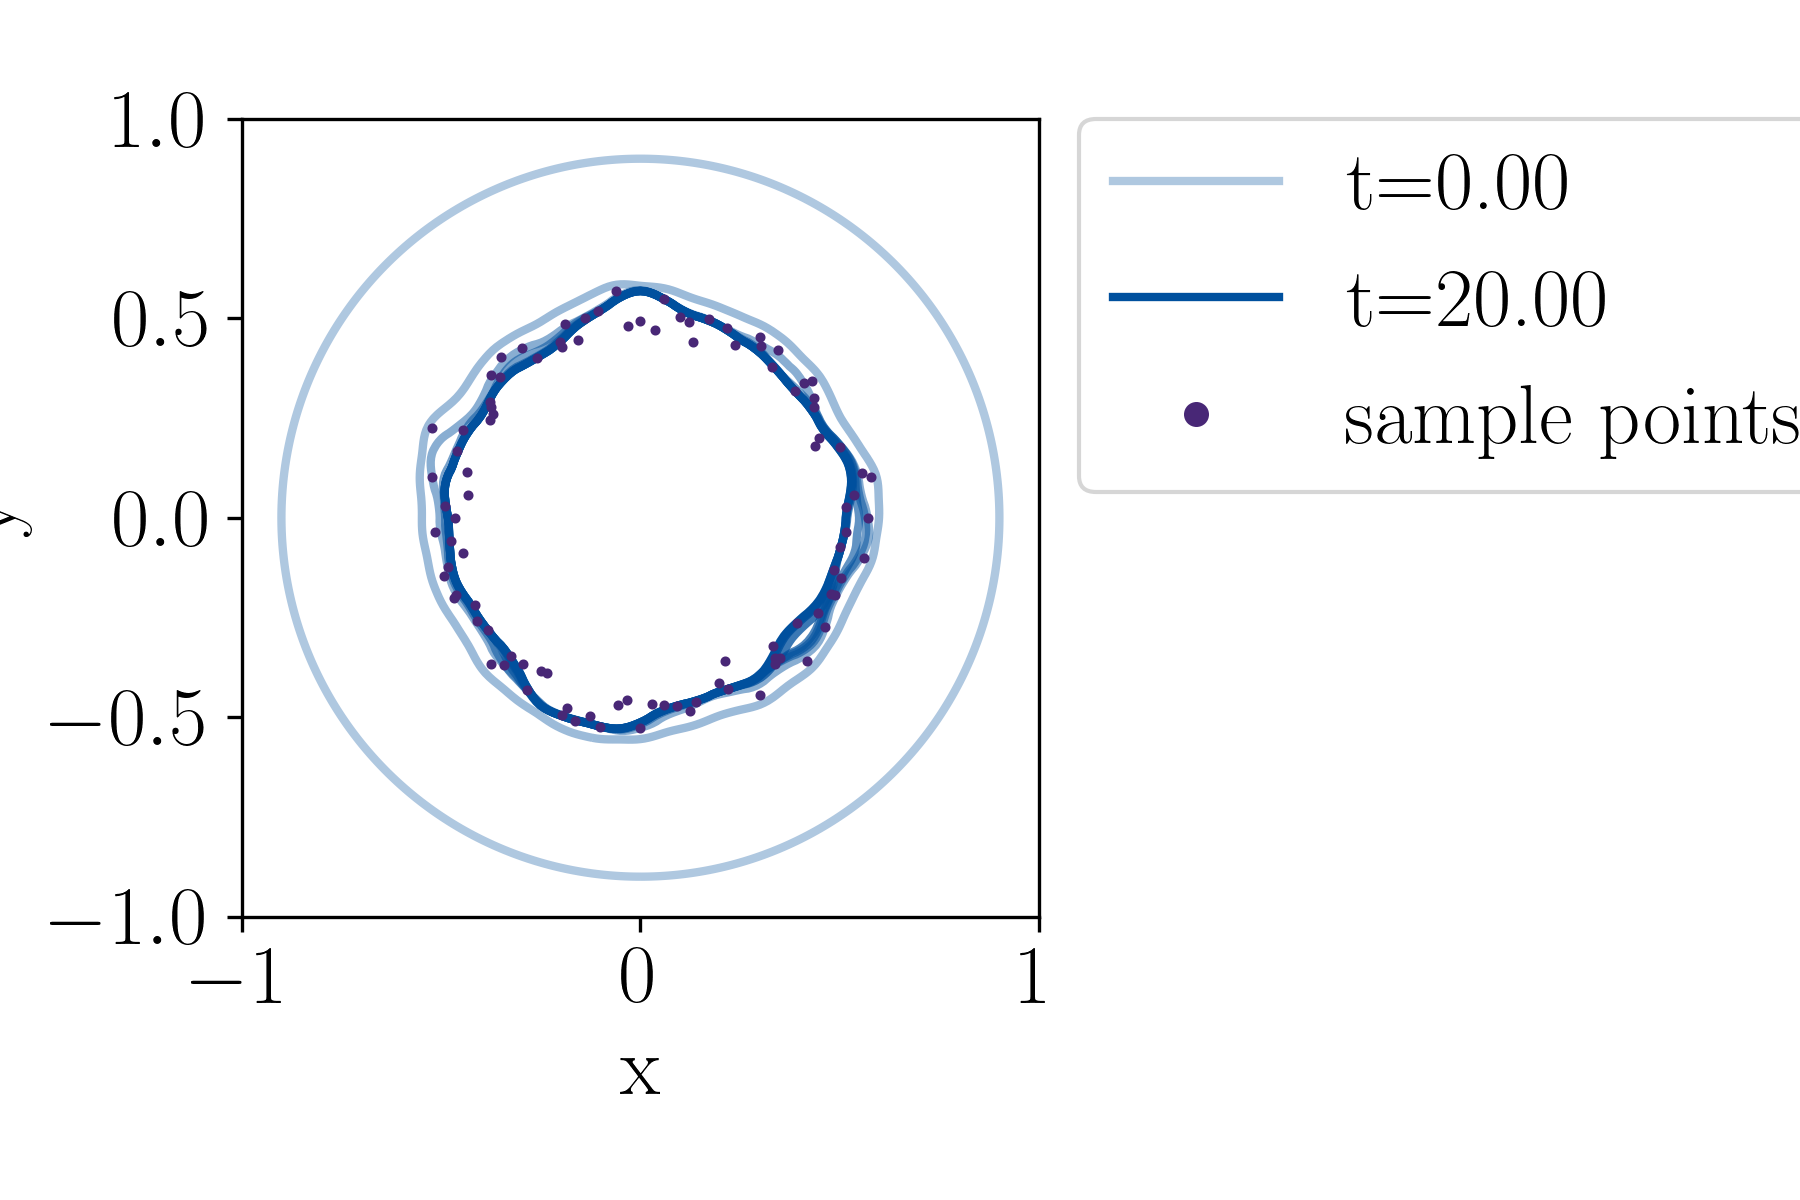
\includegraphics[height=3.5cm]{figures/Results/Noisy-points/model1/noisy-a996-t20.png}%
\,
\includegraphics[height=3.5cm]{figures/Results/Noisy-points/model1/noisy-a996-res.png}%
}
\end{center}
\vspace{-2.5em}
\caption[Model 1 - Noisy point set, $\alpha=0.999$]{Model 1: $h=0.01$, $9$ level curves, $\alpha=0.999$, $r_0=0.9$, reinitialize every $50$ steps}
\label{fig:m1-noisypoints-a999}
\end{figure}

For the second model we see in \figref{fig:m2-noisypoints-a02} that the curve fits the data quite well, not capturing the outliers on the outside nor the inside. However, the curvature at the points are much higher than for model 1, which is expected. We try to increase $\delta$ to $\delta=10^-1$ to bound the curvature near the points. We see the effect in \figref{fig:m2-noisypoints-a06} where the edges are not as sharp at the points. Since also, the distance dependent term is not as high for that choice of $\delta$, the $\alpha$-parameter is also increased. What we observe is also that the curve is again located inside the noisy band, an one might need to tune $\alpha$ even more to avoid this. However, as we now, this would again affect the curvature of the final curve. 

\begin{figure}
\begin{center}
\resizebox{.99\textwidth}{!}{%
\includegraphics[height=3.5cm]{figures/Results/Noisy-points/model2/noisypoints-a02.png}%
\,
\includegraphics[height=3.5cm]{figures/Results/Noisy-points/model2/noisy-a2-d2-res.png}%
}
\end{center}
\vspace{-2.5em}
\caption[Model 2 - Noisy point set, $\alpha=0.2$]{Model 2: $h=0.01$, $9$ level curves, $\alpha=0.2$, $r_0=0.9$, reinitialize every $50$ steps}
\label{fig:m2-noisypoints-a02}
\end{figure}

\begin{figure}
\begin{center}
\resizebox{.99\textwidth}{!}{%
\includegraphics[height=3.5cm]{figures/Results/Noisy-points/model2/noisy-a3-b1.png}%
\,
\includegraphics[height=3.5cm]{figures/Results/Noisy-points/model2/noisy-a03-d1-logy.png}%
}
\end{center}
\vspace{-2.5em}
\caption[Model 2 - Noisy point set, $\alpha=0.6$]{Model 2: $h=0.01$, $9$ level curves, $\alpha=0.6$, $r_0=0.9$, reinitialize every $50$ steps}
\label{fig:m2-noisypoints-a06}
\end{figure}

For model 3, we focus on the $\beta$-parameter, which we saw for example in the example with three equidistant points had decides the curvature near the points. 



\begin{figure}
\begin{center}
\resizebox{.99\textwidth}{!}{%
\includegraphics[height=3.5cm]{figures/Results/Noisy-points/model3/noisy-a9-b1.png}%
\,
\includegraphics[height=3.5cm]{figures/Results/Noisy-points/model3/noisy-a9-b1-res.png}%
}
\end{center}
\vspace{-2.5em}
\caption[Model 3 - Noisy point set, $\alpha=0.9$]{Model 3: $h=0.01$, $9$ level curves, $\alpha=0.9$, $r_0=0.9$, reinitialize every $50$ steps, $\beta=1$}
\label{fig:m3-noisypoints-a09}
\end{figure}

\begin{figure}
\begin{center}
\resizebox{.99\textwidth}{!}{%
\includegraphics[height=3.5cm]{figures/Results/Noisy-points/model3/noisy-a9-b3.png}%
\,
\includegraphics[height=3.5cm]{figures/Results/Noisy-points/model3/noisy-a9-b3-res.png}%
}
\end{center}
\vspace{-2.5em}
\caption[Model 3 - Noisy point set, $\alpha=0.8$]{Model 3: $h=0.01$, $9$ level curves, $\alpha=0.9$, $r_0=0.9$, reinitialize every $50$ steps, $\beta=3$}
\label{fig:m3-noisypoints-a08}
\end{figure}

\section{Summary of Results}
We have seen that all the models behave as expected for the circle. The parameter $\alpha$ scales how much the curvature affect the solution for all models. When we introduce the parameter $\delta$ for model 2, we also see that this affects the curvature of the final solution near the points. If $\delta$ is big, it "cuts off" the growing curvature, such that it the edges is not that sharp.

The parameter $\beta$ in this model 2 do not affect the maximum sharpness of the edges, but it affects the scaling of the distance. A high $\beta$ means even flatter regions further away, but it does not bound the curvature at the point. The same goes for model 3, but the curvature maximum curvature at the point is bounded by 2/pi*tan(inf)=1. 

We have seen that the tuning of the parameters are very important for all models, and using the right parameters, all models yield similar curves if the data set is dense. The difference between the models was best seen for the three points, where it was most visible how the curvature varied when the distance increased. This is also observed for test case 3 and 4 also, but since the density is so high distance to not vary as much and hence it is not as visible. 

If we now assume that we have some a priori knowledge about the underlying shape, and the sample points are picked to represent certain qualities of the curve, then one could choose a model that fits. For example, if the points are sampled where the curve is as flat as possible, model 1 is the best choice. On the other hand, if the points are sampled at something similar to edges on the underlying curve, model 2 with small $\delta$ would be preferred.

Also, model 3 has the advantage over model 2 that it has fewer parameters to tune, so the behavior of the curve is more straightforward. Although it does not have the same flexibility to tune the curvature vs distance relation.

Finally, we must discuss that none of the models reached clean stationary solutions for all problems. The reason is the local behavior of the distance function, which creates oscillations if the curve goes back and forth over the curve. Nevertheless, with the right tuning parameters, the models reached what seemed like a stationary solution, in most cases. Because problem assumes so little about the underlying shape, these fast, but very small, oscillations do not perturb the solution much, and since we do not have a right solution any of these curves would be acceptable.